\documentclass[11pt]{article}
\usepackage{fontspec}
\newcommand{\GelfandFontPath}{}
\directlua{local root=os.getenv("WINDIR"); if root then tex.sprint(string.char(92).."renewcommand{"..string.char(92).."GelfandFontPath}{"..root:gsub(string.char(92),"/").."/Fonts/}") end}
\setmainfont{NotoSerif-Regular.ttf}[Path=\GelfandFontPath,ItalicFont=NotoSerif-Italic.ttf,BoldFont=NotoSerif-Bold.ttf,BoldItalicFont=NotoSerif-BoldItalic.ttf]
\usepackage[a4paper,margin=22mm]{geometry}
\usepackage{amsmath,amssymb,graphicx,xcolor,hyperref,needspace,tikz}
\usepackage[normalem]{ulem}
\let\MathUnderline\underline
\renewcommand{\underline}[1]{\ifmmode\MathUnderline{#1}\else\uline{#1}\fi}
\hypersetup{unicode=true,colorlinks=true,linkcolor=blue,pdfauthor={}}
\setlength{\parindent}{0pt}
\setlength{\parskip}{.4em}
\setlength{\emergencystretch}{3em}
\raggedright
\newcommand{\SourcePage}[2]{\par\smallskip\phantomsection\label{#1:source-page}{\small\sffamily\color{blue!55!black}#1}\par\smallskip}
\newcommand{\EvidenceBlock}[4]{%
 \par\smallskip\noindent\begin{minipage}{\linewidth}
 \begin{minipage}[t]{.47\linewidth}\vspace{0pt}\centering
 \csname evidence-#1-#2\endcsname\par
 {\scriptsize\SourceCropCaption\ #1}\par
 \end{minipage}\hfill
 \begin{minipage}[t]{.49\linewidth}\vspace{0pt}\raggedright
 {\small\color{orange!65!black}\textbf{#4} #3}\par
 \end{minipage}
 \end{minipage}\par\smallskip}
\newcommand{\Unclear}[3]{\EvidenceBlock{#1}{#2}{#3}{\ReadingCaption}}
\newcommand{\Incomplete}[3]{\EvidenceBlock{#1}{#2}{#3}{\IncompleteCaption}}
\newcommand{\SourceFigure}[3]{\EvidenceBlock{#1}{#2}{#3}{\DiagramCaption}}
\expandafter\def\csname evidence-GELFAND-P000001-module-letter\endcsname{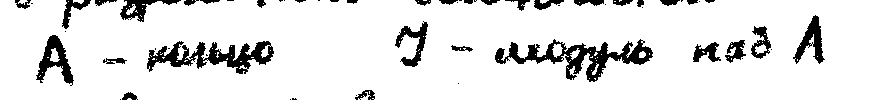
\includegraphics[width=\linewidth]{figures/gelfand-p000001-module-letter-original.png}}
\expandafter\def\csname evidence-GELFAND-P000001-diagram-blowup\endcsname{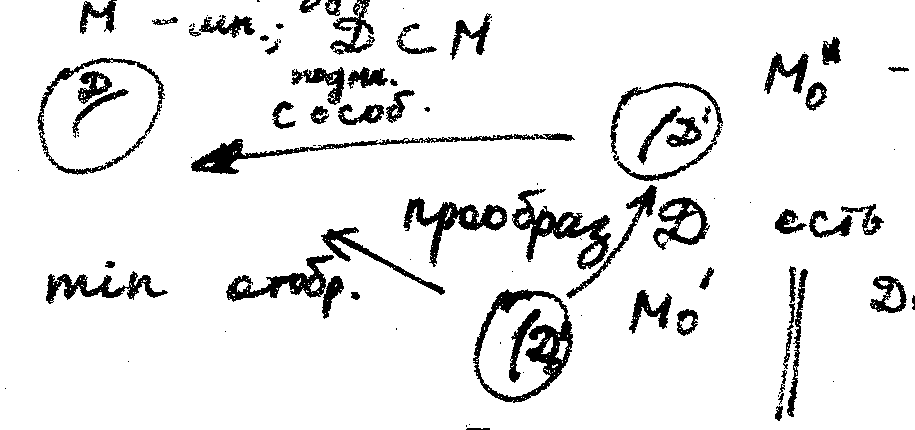
\includegraphics[width=\linewidth]{figures/gelfand-p000001-diagram-blowup-original.png}}
\expandafter\def\csname evidence-GELFAND-P000001-blowup-notation\endcsname{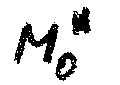
\includegraphics[width=.43\linewidth]{figures/gelfand-p000001-upper-blowup-label-original.png}\hfill
\includegraphics[width=.50\linewidth]{figures/gelfand-p000001-lower-blowup-label-original.png}}
\expandafter\def\csname evidence-GELFAND-P000001-origin-example\endcsname{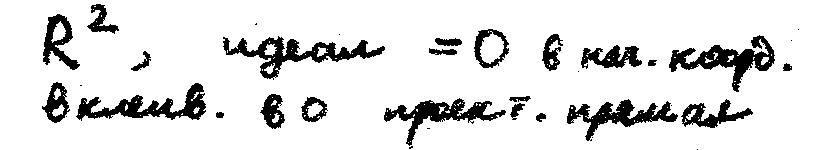
\includegraphics[width=\linewidth]{figures/gelfand-p000001-origin-example-original.png}}
\newcommand{\SourceCropCaption}{Оригинальные фрагменты:}\newcommand{\ReadingCaption}{Сомнительное чтение.}\newcommand{\IncompleteCaption}{Неразобранный фрагмент.}\newcommand{\DiagramCaption}{Рисунок и набранное описание.}
\hypersetup{pdftitle={Семинар И. М. Гельфанда — глава 1}}

\expandafter\def\csname evidence-GELFAND-P000002-ideal-selection\endcsname{
\includegraphics[width=\linewidth]{figures/gelfand-p000002-ideal-selection-part01-original-r1.png}}
\expandafter\def\csname evidence-GELFAND-P000002-open-set-notation\endcsname{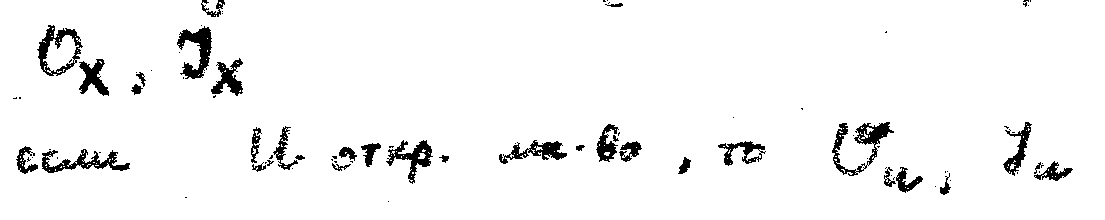
\includegraphics[width=\linewidth]{figures/gelfand-p000002-open-set-notation-part01-original-r2.png}}
\expandafter\def\csname evidence-GELFAND-P000002-fractions-sentence\endcsname{
\includegraphics[width=\linewidth]{figures/gelfand-p000002-fractions-sentence-part01-original-r1.png}\par\smallskip
\includegraphics[width=\linewidth]{figures/gelfand-p000002-fractions-sentence-part02-original-r1.png}\par\smallskip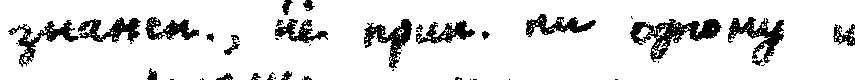
\includegraphics[width=\linewidth]{figures/gelfand-p000002-fractions-sentence-part03-original-r1.png}\par\smallskip
\includegraphics[width=\linewidth]{figures/gelfand-p000002-fractions-sentence-part04-original-r1.png}}
\expandafter\def\csname evidence-GELFAND-P000002-margin-grothendieck\endcsname{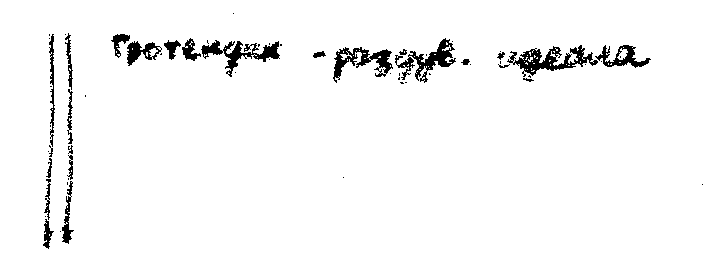
\includegraphics[width=\linewidth]{figures/gelfand-p000002-margin-grothendieck-part01-original-r1.png}}
\expandafter\def\csname evidence-GELFAND-P000002-quadratic-coefficients\endcsname{
\includegraphics[width=\linewidth]{figures/gelfand-p000002-quadratic-coefficients-part01-original-r1.png}}
\expandafter\def\csname evidence-GELFAND-P000002-last-sign\endcsname{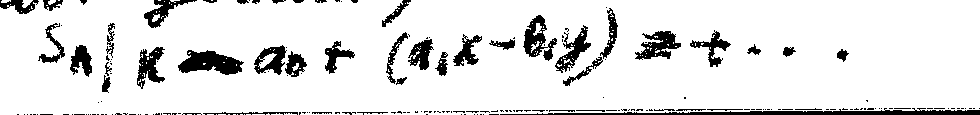
\includegraphics[width=\linewidth]{figures/gelfand-p000002-last-sign-part01-original-r1.png}}
\expandafter\def\csname evidence-GELFAND-P000003-directions\endcsname{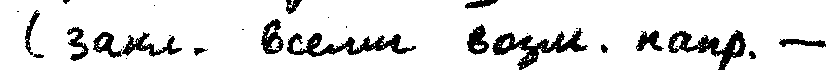
\includegraphics[width=\linewidth]{figures/gelfand-p000003-directions-part01-original-r1.png}\par\smallskip
\includegraphics[width=\linewidth]{figures/gelfand-p000003-directions-part02-original-r1.png}}
\expandafter\def\csname evidence-GELFAND-P000003-cross-cancellation\endcsname{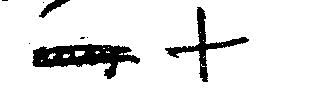
\includegraphics[width=\linewidth]{figures/gelfand-p000003-cross-cancellation-part01-original-r1.png}}
\expandafter\def\csname evidence-GELFAND-P000003-ising-cancellation\endcsname{
\includegraphics[width=\linewidth]{figures/gelfand-p000003-ising-cancellation-part01-original-r1.png}}
\expandafter\def\csname evidence-GELFAND-P000003-configuration-letter\endcsname{
\includegraphics[width=\linewidth]{figures/gelfand-p000003-configuration-letter-part01-original-r2.png}}
\expandafter\def\csname evidence-GELFAND-P000003-energy-cancellation\endcsname{
\includegraphics[width=\linewidth]{figures/gelfand-p000003-energy-cancellation-part01-original-r1.png}}
\expandafter\def\csname evidence-GELFAND-P000003-energy-case\endcsname{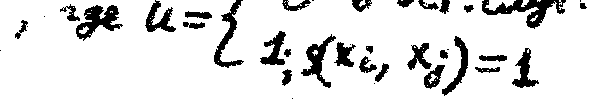
\includegraphics[width=\linewidth]{figures/gelfand-p000003-energy-case-part01-original-r2.png}\par\smallskip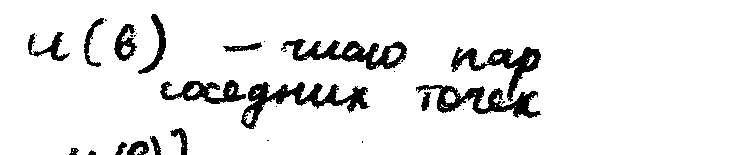
\includegraphics[width=\linewidth]{figures/gelfand-p000003-energy-case-part02-original-r3.png}}
\expandafter\def\csname evidence-GELFAND-P000003-partition-domain\endcsname{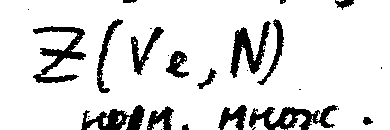
\includegraphics[width=\linewidth]{figures/gelfand-p000003-partition-domain-part01-original-r1.png}\par\smallskip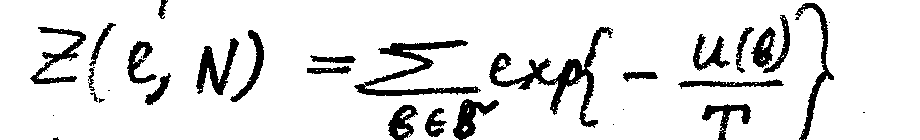
\includegraphics[width=\linewidth]{figures/gelfand-p000003-partition-domain-part02-original-r1.png}}
\expandafter\def\csname evidence-GELFAND-P000003-attraction-note\endcsname{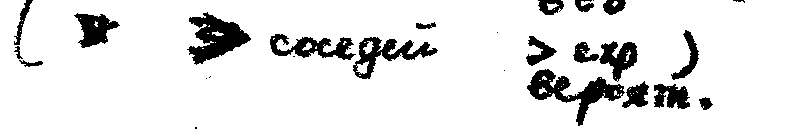
\includegraphics[width=\linewidth]{figures/gelfand-p000003-attraction-note-part01-original-r1.png}}
\expandafter\def\csname evidence-GELFAND-P000003-density-cancellation\endcsname{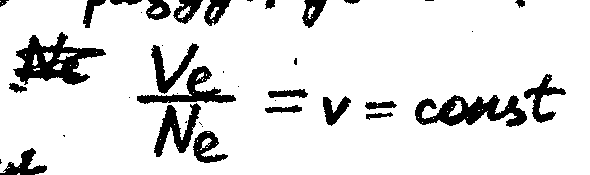
\includegraphics[width=\linewidth]{figures/gelfand-p000003-density-cancellation-part01-original-r1.png}}

\expandafter\def\csname evidence-GELFAND-P000004-pressure-letter\endcsname{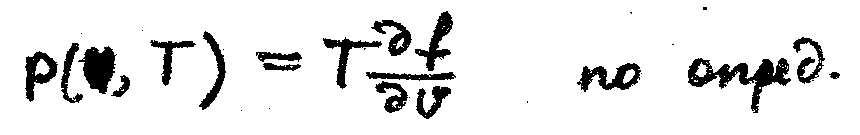
\includegraphics[width=\linewidth]{figures/gelfand-p000004-pressure-letter-part01-original-r1.png}}
\expandafter\def\csname evidence-GELFAND-P000004-diagram-phase-point\endcsname{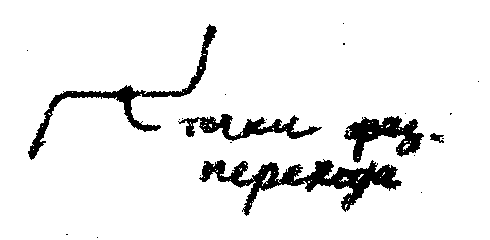
\includegraphics[width=\linewidth]{figures/gelfand-p000004-diagram-phase-point-part01-original-r2.png}}
\expandafter\def\csname evidence-GELFAND-P000004-diagram-cancelled-graph\endcsname{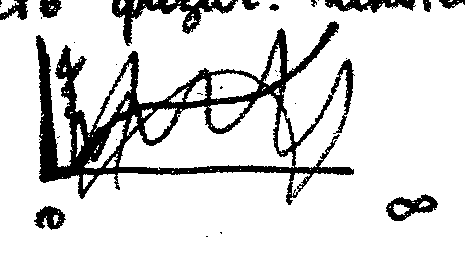
\includegraphics[width=\linewidth]{figures/gelfand-p000004-diagram-cancelled-graph-part01-original-r1.png}}
\expandafter\def\csname evidence-GELFAND-P000004-diagram-onsager\endcsname{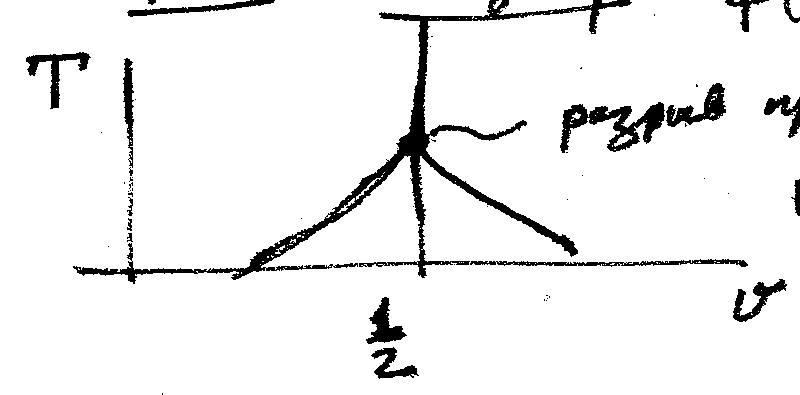
\includegraphics[width=\linewidth]{figures/gelfand-p000004-diagram-onsager-part01-original-r1.png}}
\expandafter\def\csname evidence-GELFAND-P000004-kac-helfand-note\endcsname{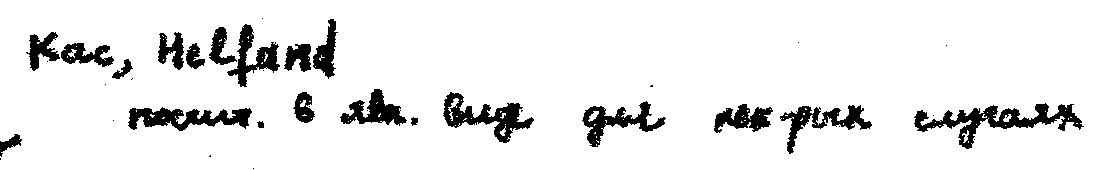
\includegraphics[width=\linewidth]{figures/gelfand-p000004-kac-helfand-note-part01-original-r1.png}}
\expandafter\def\csname evidence-GELFAND-P000004-diagram-subcube\endcsname{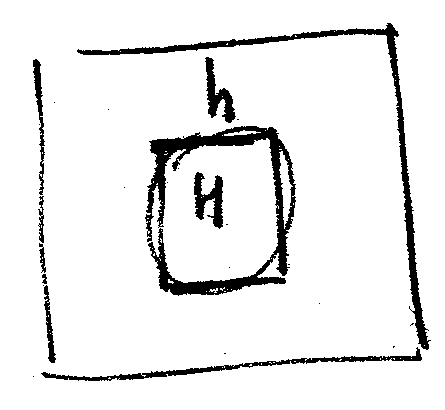
\includegraphics[width=\linewidth]{figures/gelfand-p000004-diagram-subcube-part01-original-r1.png}}
\expandafter\def\csname evidence-GELFAND-P000004-probability-bar\endcsname{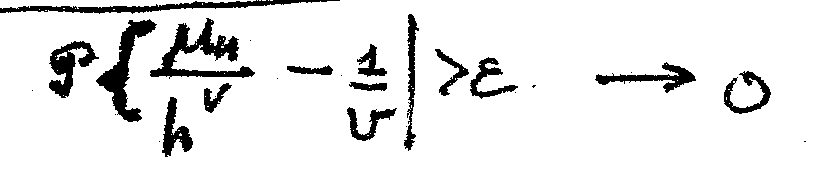
\includegraphics[width=\linewidth]{figures/gelfand-p000004-probability-bar-part01-original-r1.png}}
\expandafter\def\csname evidence-GELFAND-P000004-bottom-mark\endcsname{
\includegraphics[width=\linewidth]{figures/gelfand-p000004-bottom-mark-part01-original-r1.png}}
\expandafter\def\csname evidence-GELFAND-P000004-margin-left\endcsname{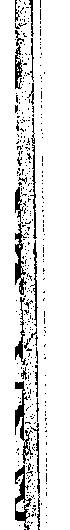
\includegraphics[height=60mm]{figures/gelfand-p000004-margin-left-part01-original-r1.png}\hspace{2mm}
\includegraphics[height=60mm]{figures/gelfand-p000004-margin-left-part02-original-r1.png}\hspace{2mm}
\includegraphics[height=60mm]{figures/gelfand-p000004-margin-left-part03-original-r1.png}\hspace{2mm}
\includegraphics[height=60mm]{figures/gelfand-p000004-margin-left-part04-original-r1.png}}
\expandafter\def\csname evidence-GELFAND-P000005-exponential-rate\endcsname{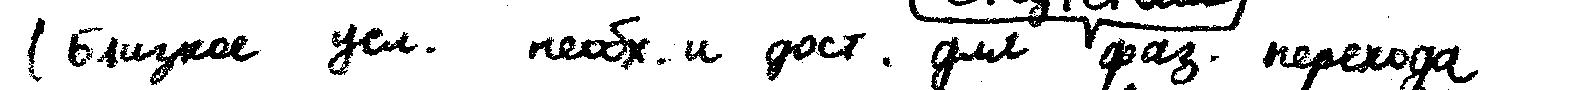
\includegraphics[width=\linewidth]{figures/gelfand-p000005-exponential-rate-part01-original-r1.png}\par\smallskip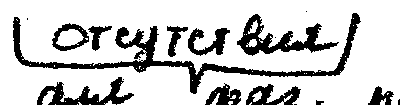
\includegraphics[width=\linewidth]{figures/gelfand-p000005-exponential-rate-part02-original-r1.png}\par\smallskip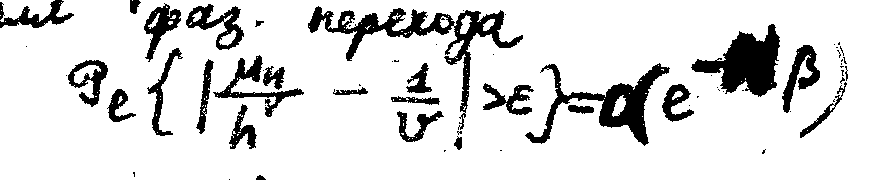
\includegraphics[width=\linewidth]{figures/gelfand-p000005-exponential-rate-part03-original-r2.png}}
\expandafter\def\csname evidence-GELFAND-P000005-complement-label\endcsname{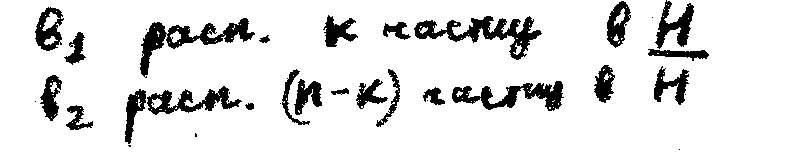
\includegraphics[width=\linewidth]{figures/gelfand-p000005-complement-label-part01-original-r1.png}}
\expandafter\def\csname evidence-GELFAND-P000005-boundary-exponent\endcsname{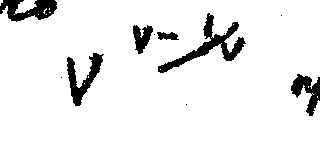
\includegraphics[width=\linewidth]{figures/gelfand-p000005-boundary-exponent-part01-original-r1.png}\par\smallskip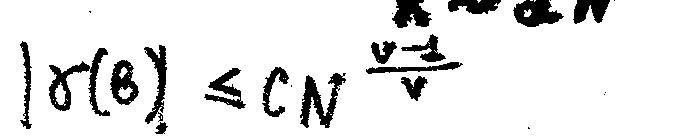
\includegraphics[width=\linewidth]{figures/gelfand-p000005-boundary-exponent-part02-original-r1.png}}
\expandafter\def\csname evidence-GELFAND-P000005-theta-factor\endcsname{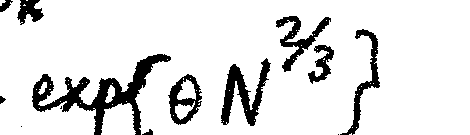
\includegraphics[width=\linewidth]{figures/gelfand-p000005-theta-factor-part01-original-r1.png}\par\smallskip
\includegraphics[width=\linewidth]{figures/gelfand-p000005-theta-factor-part02-original-r1.png}\par\smallskip
\includegraphics[width=\linewidth]{figures/gelfand-p000005-theta-factor-part03-original-r1.png}}
\expandafter\def\csname evidence-GELFAND-P000005-physical-meaning-heading\endcsname{
\includegraphics[width=\linewidth]{figures/gelfand-p000005-physical-meaning-heading-part01-original-r1.png}}
\expandafter\def\csname evidence-GELFAND-P000004-diagram-pressure-plateau\endcsname{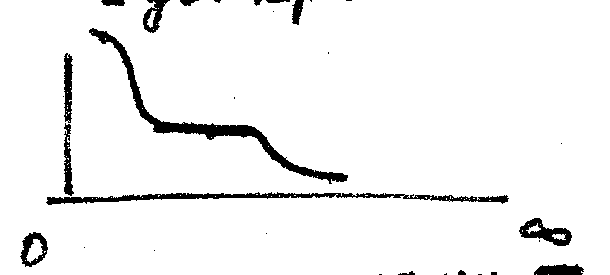
\includegraphics[width=\linewidth]{figures/gelfand-p000004-diagram-pressure-plateau-original-r1.png}}
\newcommand{\PhaseWords}{точки фаз.\\перехода}

\expandafter\def\csname evidence-GELFAND-P000006-subcube-power\endcsname{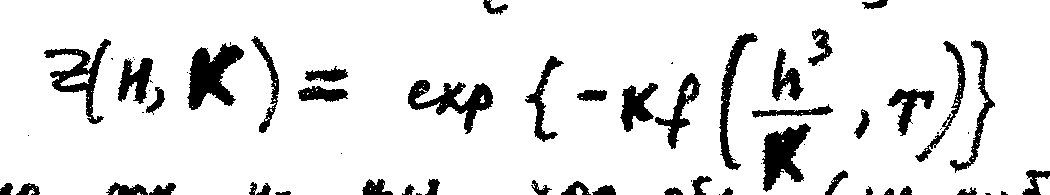
\includegraphics[width=\linewidth]{figures/gelfand-p000006-subcube-power-part01-original-r1.png}\par\smallskip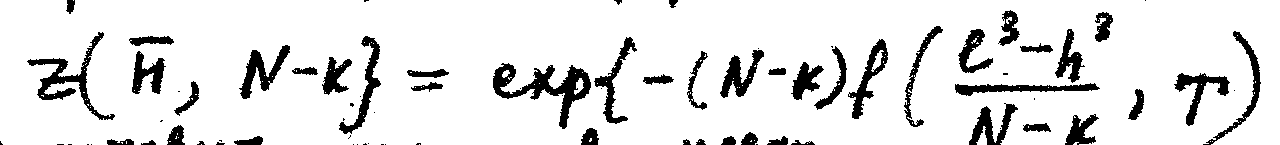
\includegraphics[width=\linewidth]{figures/gelfand-p000006-subcube-power-part02-original-r1.png}}
\expandafter\def\csname evidence-GELFAND-P000006-limit-notation\endcsname{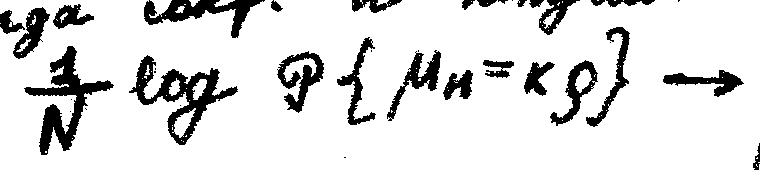
\includegraphics[width=\linewidth]{figures/gelfand-p000006-limit-notation-part01-original-r1.png}\par\smallskip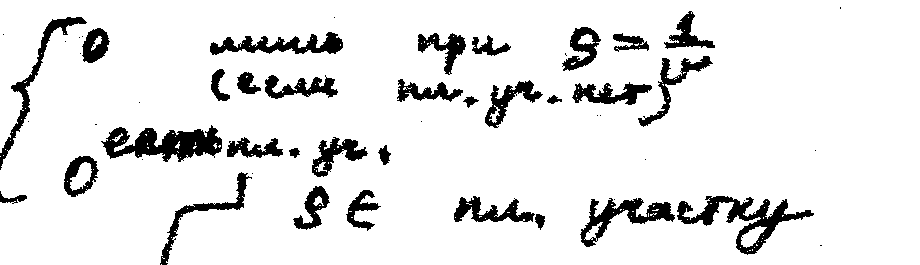
\includegraphics[width=\linewidth]{figures/gelfand-p000006-limit-notation-part02-original-r1.png}}
\expandafter\def\csname evidence-GELFAND-P000006-diagram-limit-step\endcsname{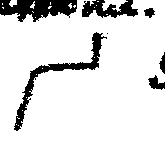
\includegraphics[width=\linewidth]{figures/gelfand-p000006-diagram-limit-step-part01-original-r1.png}}
\expandafter\def\csname evidence-GELFAND-P000006-diagram-cell-clusters\endcsname{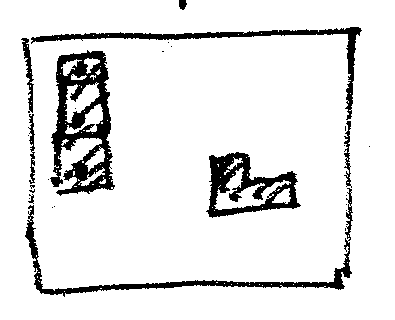
\includegraphics[width=\linewidth]{figures/gelfand-p000006-diagram-cell-clusters-part01-original-r1.png}}
\expandafter\def\csname evidence-GELFAND-P000006-gamma-prime\endcsname{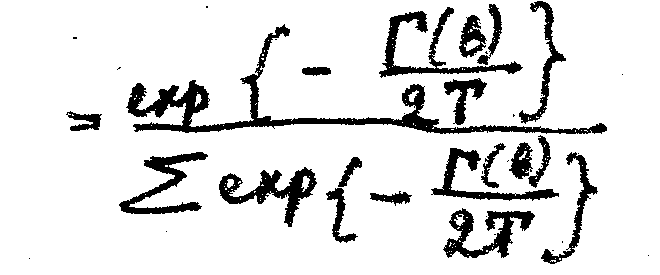
\includegraphics[width=\linewidth]{figures/gelfand-p000006-gamma-prime-part01-original-r1.png}}
\expandafter\def\csname evidence-GELFAND-P000006-energy-bound\endcsname{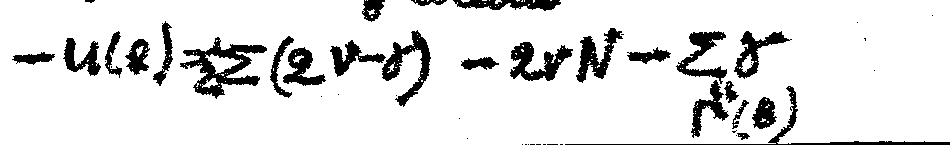
\includegraphics[width=\linewidth]{figures/gelfand-p000006-energy-bound-part01-original-r1.png}}
\expandafter\def\csname evidence-GELFAND-P000007-diagram-small-clusters\endcsname{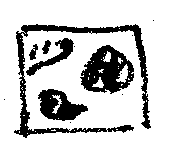
\includegraphics[width=\linewidth]{figures/gelfand-p000007-diagram-small-clusters-part01-original-r1.png}}
\expandafter\def\csname evidence-GELFAND-P000007-diagram-cycles\endcsname{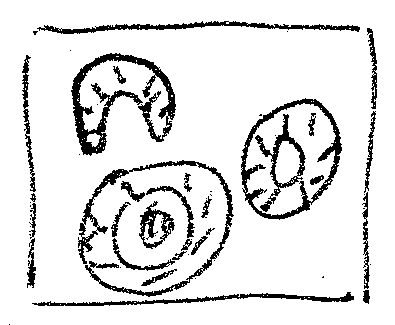
\includegraphics[width=\linewidth]{figures/gelfand-p000007-diagram-cycles-part01-original-r1.png}}
\expandafter\def\csname evidence-GELFAND-P000007-special-arrangement-count\endcsname{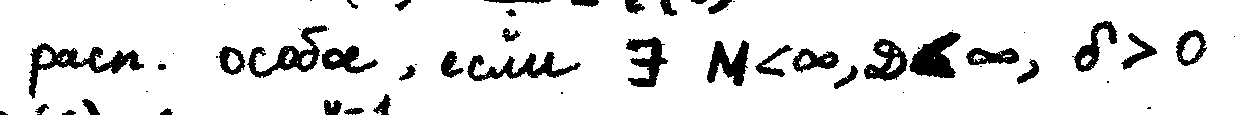
\includegraphics[width=\linewidth]{figures/gelfand-p000007-special-arrangement-count-part01-original-r1.png}}
\expandafter\def\csname evidence-GELFAND-P000007-large-cycles-power\endcsname{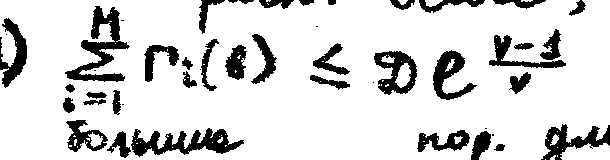
\includegraphics[width=\linewidth]{figures/gelfand-p000007-large-cycles-power-part01-original-r1.png}}
\expandafter\def\csname evidence-GELFAND-P000007-small-cycles-sum\endcsname{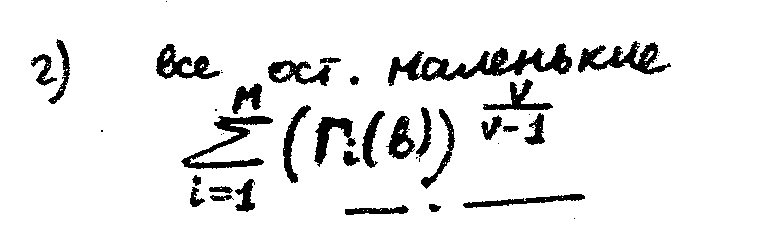
\includegraphics[width=\linewidth]{figures/gelfand-p000007-small-cycles-sum-part01-original-r1.png}}
\expandafter\def\csname evidence-GELFAND-P000007-field-margin\endcsname{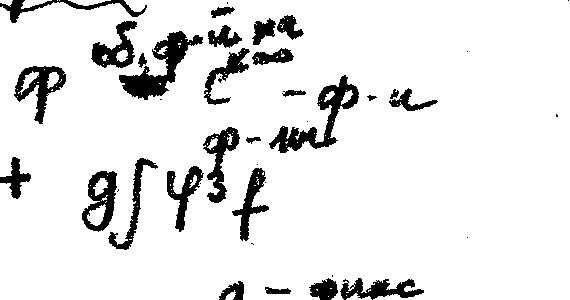
\includegraphics[width=\linewidth]{figures/gelfand-p000007-field-margin-part01-original-r1.png}}
\expandafter\def\csname evidence-GELFAND-P000007-evaluation-target\endcsname{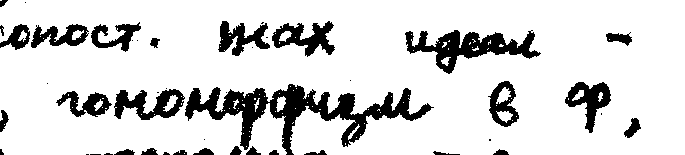
\includegraphics[width=\linewidth]{figures/gelfand-p000007-evaluation-target-part01-original-r1.png}}
\expandafter\def\csname evidence-GELFAND-P000008-linear-oscillation\endcsname{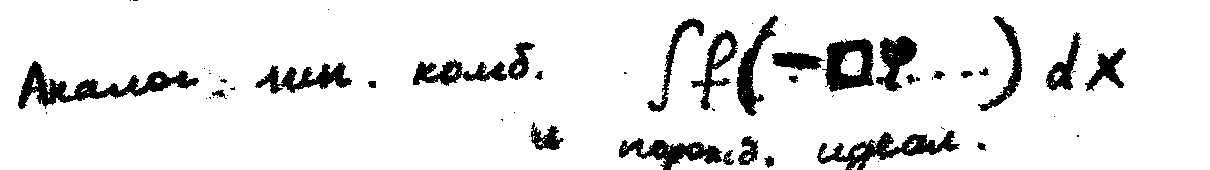
\includegraphics[width=\linewidth]{figures/gelfand-p000008-linear-oscillation-part01-original-r1.png}}
\expandafter\def\csname evidence-GELFAND-P000008-name-van-hove\endcsname{
\includegraphics[width=\linewidth]{figures/gelfand-p000008-name-van-hove-part01-original-r1.png}}
\expandafter\def\csname evidence-GELFAND-P000008-temperature-relation\endcsname{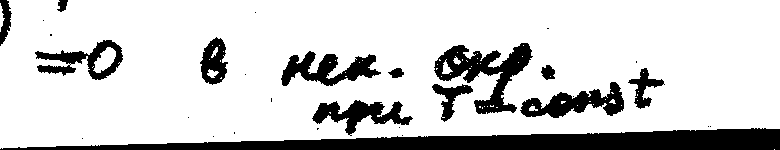
\includegraphics[width=\linewidth]{figures/gelfand-p000008-temperature-relation-part01-original-r1.png}}
\expandafter\def\csname evidence-GELFAND-P000008-margin-left\endcsname{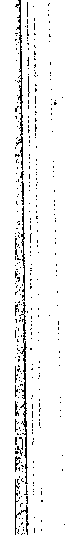
\includegraphics[height=60mm]{figures/gelfand-p000008-margin-left-part01-original-r1.png}\hspace{2mm}
\includegraphics[height=60mm]{figures/gelfand-p000008-margin-left-part02-original-r1.png}\hspace{2mm}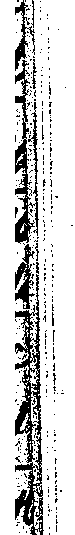
\includegraphics[height=60mm]{figures/gelfand-p000008-margin-left-part03-original-r1.png}\hspace{2mm}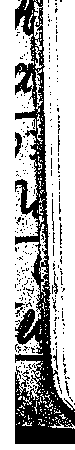
\includegraphics[height=60mm]{figures/gelfand-p000008-margin-left-part04-original-r1.png}}
\expandafter\def\csname evidence-GELFAND-P000009-sphere-constant\endcsname{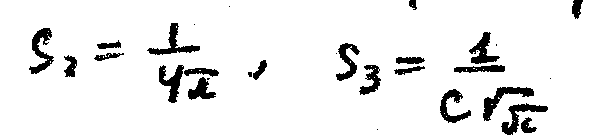
\includegraphics[width=\linewidth]{figures/gelfand-p000009-sphere-constant-part01-original-r1.png}}
\expandafter\def\csname evidence-GELFAND-P000009-probability-brace\endcsname{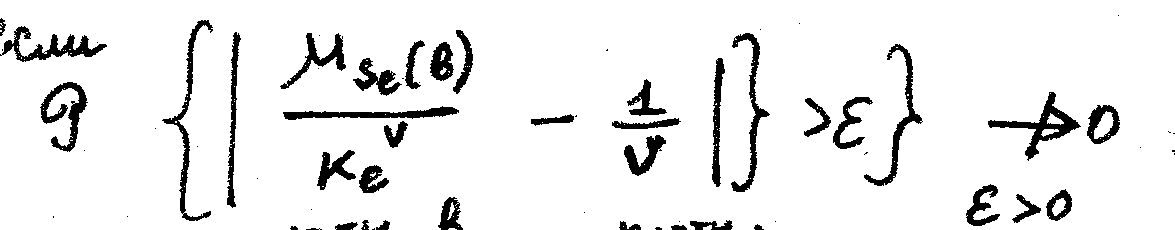
\includegraphics[width=\linewidth]{figures/gelfand-p000009-probability-brace-part01-original-r1.png}}
\expandafter\def\csname evidence-GELFAND-P000010-diagram-nested-cycles\endcsname{
\includegraphics[width=\linewidth]{figures/gelfand-p000010-diagram-nested-cycles-part01-original-r1.png}}
\expandafter\def\csname evidence-GELFAND-P000010-diagram-phase-mixture\endcsname{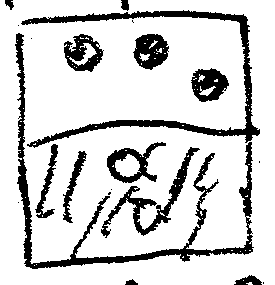
\includegraphics[width=\linewidth]{figures/gelfand-p000010-diagram-phase-mixture-part01-original-r1.png}}
\expandafter\def\csname evidence-GELFAND-P000007-ideal-signature\endcsname{
\includegraphics[width=\linewidth]{figures/gelfand-p000007-ideal-signature-part01-original-r2.png}}
\expandafter\def\csname evidence-GELFAND-P000008-algebra-ring-letter\endcsname{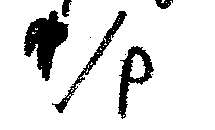
\includegraphics[width=\linewidth]{figures/gelfand-p000008-algebra-ring-letter-part01-original-r2.png}\par\smallskip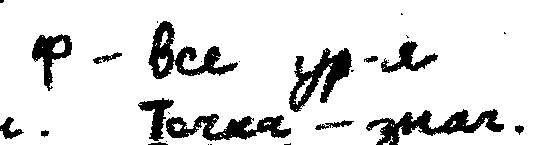
\includegraphics[width=\linewidth]{figures/gelfand-p000008-algebra-ring-letter-part02-original-r2.png}}
\expandafter\def\csname evidence-GELFAND-P000009-q-formula\endcsname{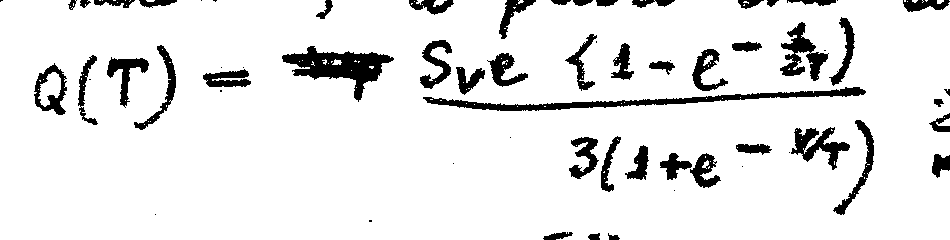
\includegraphics[width=\linewidth]{figures/gelfand-p000009-q-formula-part01-original-r2.png}\par\smallskip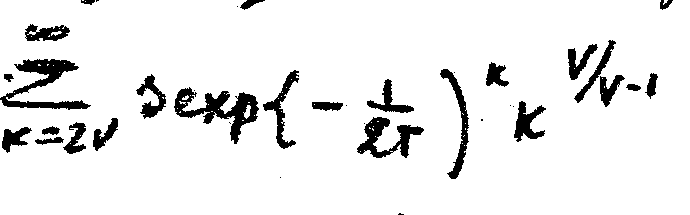
\includegraphics[width=\linewidth]{figures/gelfand-p000009-q-formula-part02-original-r2.png}}
\expandafter\def\csname evidence-GELFAND-P000009-finite-parameter\endcsname{
\includegraphics[width=\linewidth]{figures/gelfand-p000009-finite-parameter-part01-original-r2.png}}
\expandafter\def\csname evidence-GELFAND-P000010-small-cycles-sign\endcsname{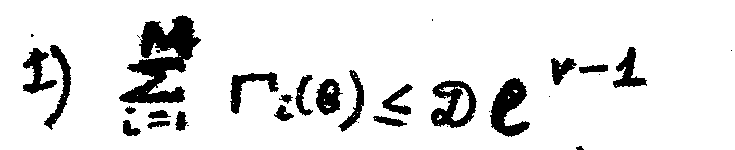
\includegraphics[width=\linewidth]{figures/gelfand-p000010-small-cycles-sign-part01-original-r2.png}\par\smallskip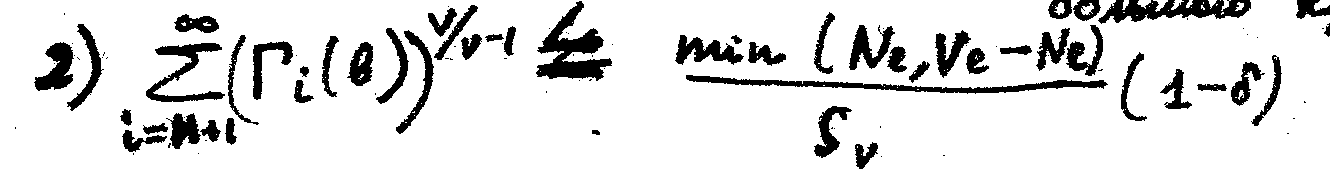
\includegraphics[width=\linewidth]{figures/gelfand-p000010-small-cycles-sign-part02-original-r2.png}}
\expandafter\def\csname evidence-GELFAND-P000010-small-volume-cancellation\endcsname{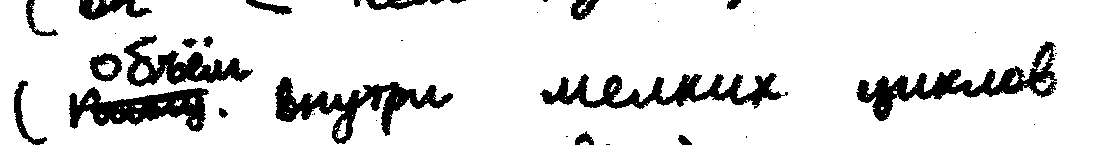
\includegraphics[width=\linewidth]{figures/gelfand-p000010-small-volume-cancellation-part01-original-r2.png}\par\smallskip
\includegraphics[width=\linewidth]{figures/gelfand-p000010-small-volume-cancellation-part02-original-r2.png}\par\smallskip
\includegraphics[width=\linewidth]{figures/gelfand-p000010-small-volume-cancellation-part03-original-r2.png}}
\expandafter\def\csname evidence-GELFAND-P000010-theorem-condition\endcsname{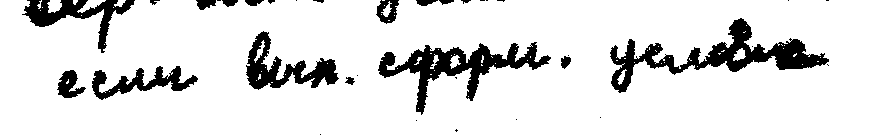
\includegraphics[width=\linewidth]{figures/gelfand-p000010-theorem-condition-part01-original-r2.png}}
\expandafter\def\csname evidence-GELFAND-P000010-diagram-grid\endcsname{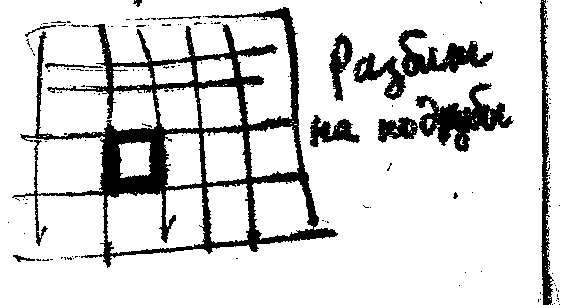
\includegraphics[width=\linewidth]{figures/gelfand-p000010-diagram-grid-part01-original-r2.png}}
\expandafter\def\csname evidence-GELFAND-P000010-last-fraction\endcsname{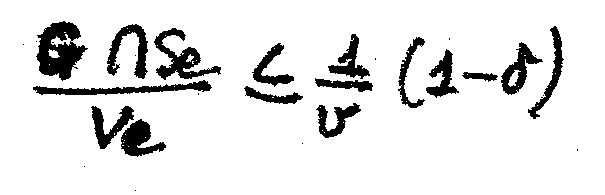
\includegraphics[width=\linewidth]{figures/gelfand-p000010-last-fraction-part01-original-r2.png}}
\expandafter\def\csname evidence-GELFAND-P000008-diagram-three-cells\endcsname{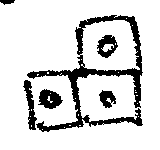
\includegraphics[width=\linewidth]{figures/gelfand-p000008-diagram-three-cells-part01-original-r1.png}}
\expandafter\def\csname evidence-GELFAND-P000009-diagram-corner-cluster\endcsname{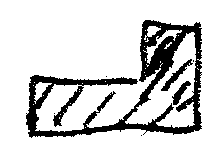
\includegraphics[width=\linewidth]{figures/gelfand-p000009-diagram-corner-cluster-part01-original-r1.png}}
\expandafter\def\csname evidence-GELFAND-P000009-diagram-coexistence-dome\endcsname{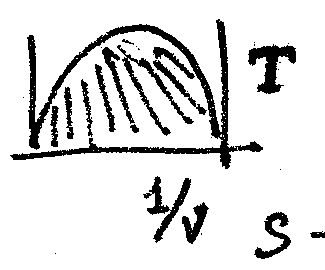
\includegraphics[width=\linewidth]{figures/gelfand-p000009-diagram-coexistence-dome-part01-original-r2.png}}
\newcommand{\GridWords}{Разбили\\на подкубы}

\expandafter\def\csname evidence-GELFAND-P000011-top-line\endcsname{
\includegraphics[width=\linewidth]{figures/gelfand-p000011-top-line-part01-original-r1.png}}
\expandafter\def\csname evidence-GELFAND-P000011-diagram-01\endcsname{
\includegraphics[width=\linewidth]{figures/gelfand-p000011-diagram-01-part01-original-r1.png}}
\expandafter\def\csname evidence-GELFAND-P000011-upper-middle\endcsname{
\includegraphics[width=\linewidth]{figures/gelfand-p000011-upper-middle-part01-original-r1.png}}
\expandafter\def\csname evidence-GELFAND-P000011-upper-right-cancellation\endcsname{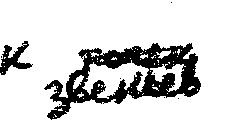
\includegraphics[width=\linewidth]{figures/gelfand-p000011-upper-right-cancellation-part01-original-r1.png}}
\expandafter\def\csname evidence-GELFAND-P000011-diagram-02\endcsname{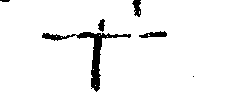
\includegraphics[width=\linewidth]{figures/gelfand-p000011-diagram-02-part01-original-r1.png}}
\expandafter\def\csname evidence-GELFAND-P000011-middle-cancellation-01\endcsname{
\includegraphics[width=\linewidth]{figures/gelfand-p000011-middle-cancellation-01-part01-original-r1.png}}
\expandafter\def\csname evidence-GELFAND-P000011-middle-cancellation-02\endcsname{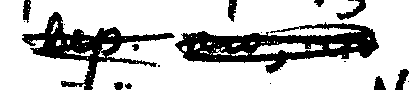
\includegraphics[width=\linewidth]{figures/gelfand-p000011-middle-cancellation-02-part01-original-r1.png}}
\expandafter\def\csname evidence-GELFAND-P000011-middle-bound\endcsname{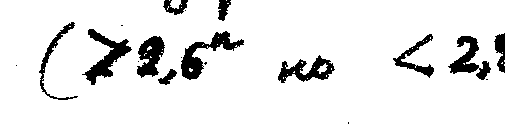
\includegraphics[width=\linewidth]{figures/gelfand-p000011-middle-bound-balanced-part01-original-r4.png}\par\smallskip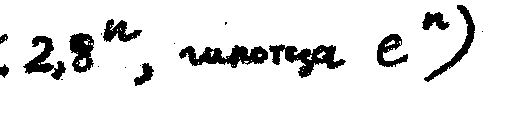
\includegraphics[width=\linewidth]{figures/gelfand-p000011-middle-bound-balanced-part02-original-r4.png}}
\expandafter\def\csname evidence-GELFAND-P000011-bottom-line\endcsname{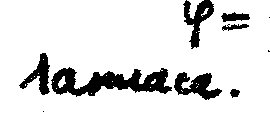
\includegraphics[width=\linewidth]{figures/gelfand-p000011-bottom-line-part01-original-r1.png}}
\expandafter\def\csname evidence-GELFAND-P000012-upper-norm\endcsname{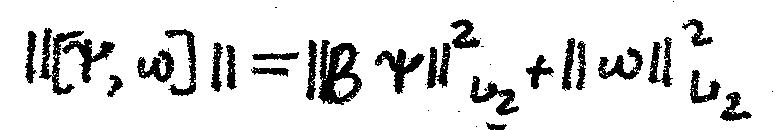
\includegraphics[width=\linewidth]{figures/gelfand-p000012-upper-norm-part01-original-r1.png}}
\expandafter\def\csname evidence-GELFAND-P000012-upper-selfadjoint\endcsname{
\includegraphics[width=\linewidth]{figures/gelfand-p000012-upper-selfadjoint-balanced-part01-original-r4.png}\par\smallskip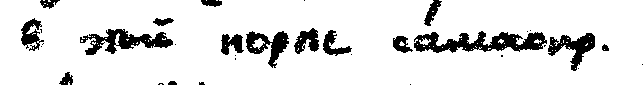
\includegraphics[width=\linewidth]{figures/gelfand-p000012-upper-selfadjoint-balanced-part02-original-r4.png}}
\expandafter\def\csname evidence-GELFAND-P000012-upper-right-note\endcsname{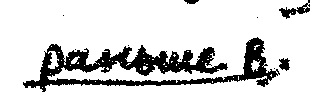
\includegraphics[width=\linewidth]{figures/gelfand-p000012-upper-right-note-part01-original-r1.png}}
\expandafter\def\csname evidence-GELFAND-P000012-middle-cancellation\endcsname{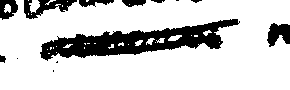
\includegraphics[width=\linewidth]{figures/gelfand-p000012-middle-cancellation-part01-original-r1.png}}
\expandafter\def\csname evidence-GELFAND-P000012-middle-right-note\endcsname{
\includegraphics[width=\linewidth]{figures/gelfand-p000012-middle-right-note-part01-original-r1.png}}
\expandafter\def\csname evidence-GELFAND-P000012-lower-variation\endcsname{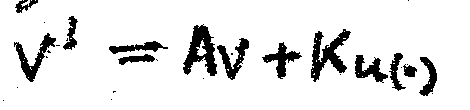
\includegraphics[width=\linewidth]{figures/gelfand-p000012-lower-variation-part01-original-r1.png}}
\expandafter\def\csname evidence-GELFAND-P000013-top-line\endcsname{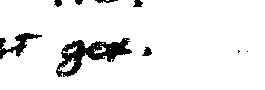
\includegraphics[width=\linewidth]{figures/gelfand-p000013-top-line-part01-original-r1.png}}
\expandafter\def\csname evidence-GELFAND-P000014-upper-borel-note\endcsname{
\includegraphics[width=\linewidth]{figures/gelfand-p000014-upper-borel-note-part01-original-r1.png}}
\expandafter\def\csname evidence-GELFAND-P000014-middle-cancellation-01\endcsname{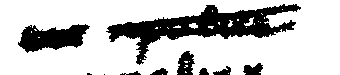
\includegraphics[width=\linewidth]{figures/gelfand-p000014-middle-cancellation-01-part01-original-r1.png}}
\expandafter\def\csname evidence-GELFAND-P000014-middle-uniqueness\endcsname{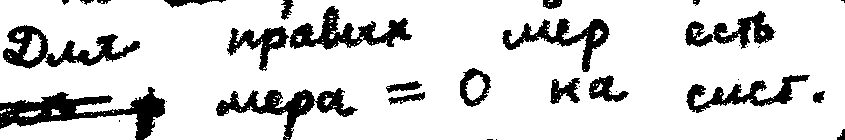
\includegraphics[width=\linewidth]{figures/gelfand-p000014-middle-uniqueness-balanced-part01-original-r4.png}\par\smallskip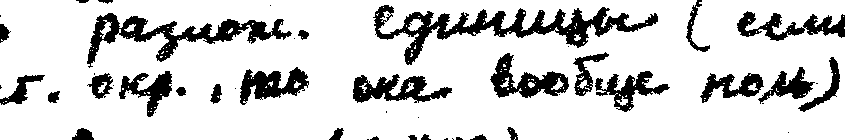
\includegraphics[width=\linewidth]{figures/gelfand-p000014-middle-uniqueness-balanced-part02-original-r4.png}}
\expandafter\def\csname evidence-GELFAND-P000014-middle-cancellation-02\endcsname{
\includegraphics[width=\linewidth]{figures/gelfand-p000014-middle-cancellation-02-part01-original-r1.png}}
\expandafter\def\csname evidence-GELFAND-P000014-lower-set-names\endcsname{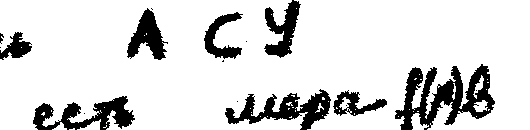
\includegraphics[width=\linewidth]{figures/gelfand-p000014-lower-set-names-balanced-part01-original-r4.png}\par\smallskip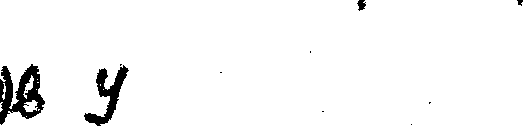
\includegraphics[width=\linewidth]{figures/gelfand-p000014-lower-set-names-balanced-part02-original-r4.png}\par\smallskip
\includegraphics[width=\linewidth]{figures/gelfand-p000014-lower-set-names-balanced-part03-original-r4.png}\par\smallskip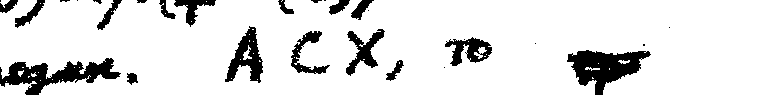
\includegraphics[width=\linewidth]{figures/gelfand-p000014-lower-set-names-balanced-part04-original-r4.png}\par\smallskip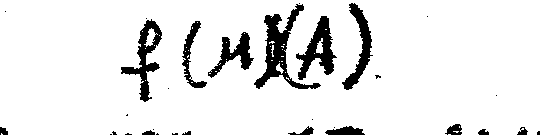
\includegraphics[width=\linewidth]{figures/gelfand-p000014-lower-set-names-balanced-part05-original-r4.png}\par\smallskip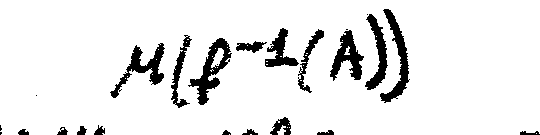
\includegraphics[width=\linewidth]{figures/gelfand-p000014-lower-set-names-balanced-part06-original-r4.png}}
\expandafter\def\csname evidence-GELFAND-P000014-lower-cancellation\endcsname{
\includegraphics[width=\linewidth]{figures/gelfand-p000014-lower-cancellation-part01-original-r1.png}}
\expandafter\def\csname evidence-GELFAND-P000015-upper-null-note\endcsname{
\includegraphics[width=\linewidth]{figures/gelfand-p000015-upper-null-note-part01-original-r1.png}}
\expandafter\def\csname evidence-GELFAND-P000015-lower-regularity\endcsname{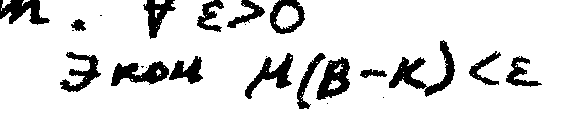
\includegraphics[width=\linewidth]{figures/gelfand-p000015-lower-regularity-part01-original-r1.png}}
\expandafter\def\csname evidence-GELFAND-P000015-bottom-cancellation\endcsname{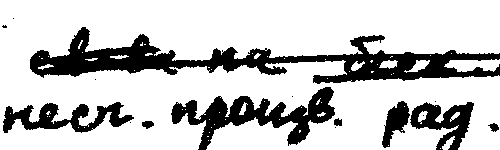
\includegraphics[width=\linewidth]{figures/gelfand-p000015-bottom-cancellation-balanced-part01-original-r4.png}\par\smallskip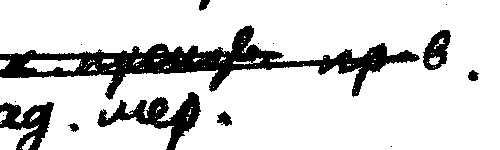
\includegraphics[width=\linewidth]{figures/gelfand-p000015-bottom-cancellation-balanced-part02-original-r4.png}}
\expandafter\def\csname evidence-GELFAND-P000015-upper-lebesgue-notation\endcsname{
\includegraphics[width=\linewidth]{figures/gelfand-p000015-upper-lebesgue-notation-part01-original-r1.png}}
\expandafter\def\csname evidence-GELFAND-P000015-upper-regularity\endcsname{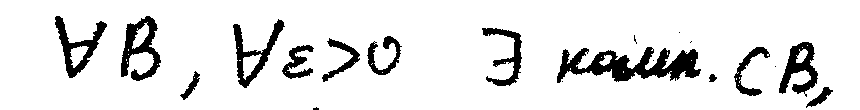
\includegraphics[width=\linewidth]{figures/gelfand-p000015-upper-regularity-part01-original-r1.png}\par\smallskip
\includegraphics[width=\linewidth]{figures/gelfand-p000015-upper-regularity-part02-original-r1.png}}
\expandafter\def\csname evidence-GELFAND-P000013-middle-commutator\endcsname{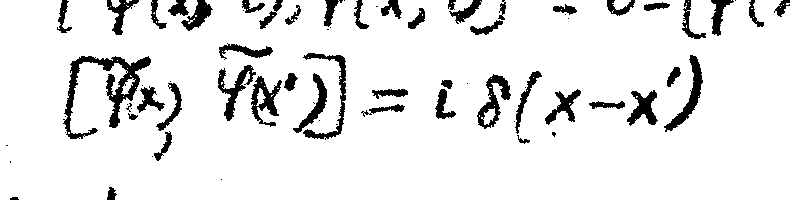
\includegraphics[width=\linewidth]{figures/gelfand-p000013-middle-commutator-part01-original-r2.png}}

\expandafter\def\csname evidence-GELFAND-P000016-upper-space-symbol\endcsname{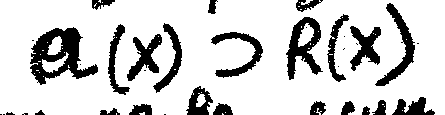
\includegraphics[width=\linewidth]{figures/gelfand-p000016-upper-space-symbol-part01-original-r1.png}}
\expandafter\def\csname evidence-GELFAND-P000016-middle-universal\endcsname{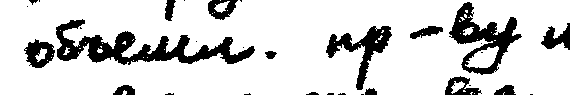
\includegraphics[width=\linewidth]{figures/gelfand-p000016-middle-universal-part01-original-r1.png}}
\expandafter\def\csname evidence-GELFAND-P000016-lower-operator-space\endcsname{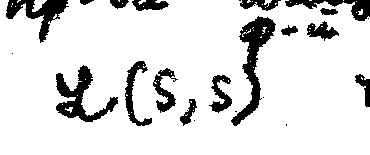
\includegraphics[width=\linewidth]{figures/gelfand-p000016-lower-operator-space-part01-original-r1.png}}
\expandafter\def\csname evidence-GELFAND-P000017-middle-group-hypothesis\endcsname{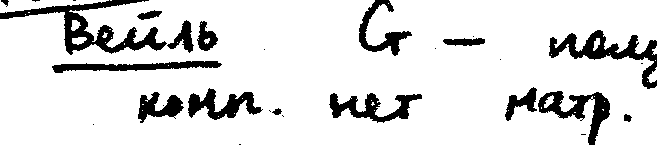
\includegraphics[width=\linewidth]{figures/gelfand-p000017-middle-group-hypothesis-part01-original-r1.png}\par\smallskip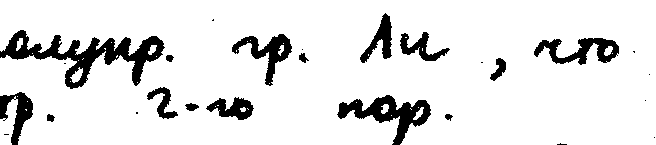
\includegraphics[width=\linewidth]{figures/gelfand-p000017-middle-group-hypothesis-part02-original-r1.png}\par\smallskip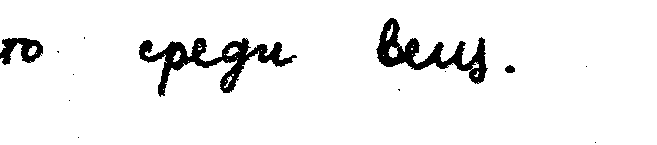
\includegraphics[width=\linewidth]{figures/gelfand-p000017-middle-group-hypothesis-part03-original-r1.png}}
\expandafter\def\csname evidence-GELFAND-P000017-lower-nondiscrete\endcsname{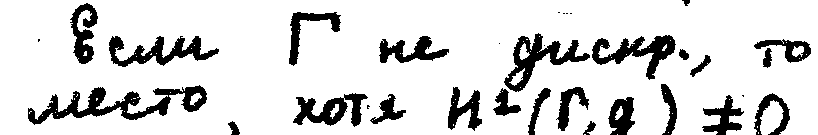
\includegraphics[width=\linewidth]{figures/gelfand-p000017-lower-nondiscrete-part01-original-r1.png}\par\smallskip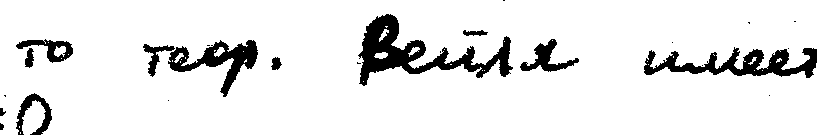
\includegraphics[width=\linewidth]{figures/gelfand-p000017-lower-nondiscrete-part02-original-r1.png}}
\expandafter\def\csname evidence-GELFAND-P000018-upper-example\endcsname{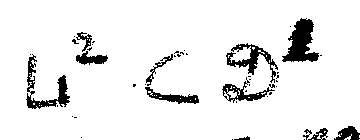
\includegraphics[width=\linewidth]{figures/gelfand-p000018-upper-example-part01-original-r1.png}}
\expandafter\def\csname evidence-GELFAND-P000018-bottom-norm\endcsname{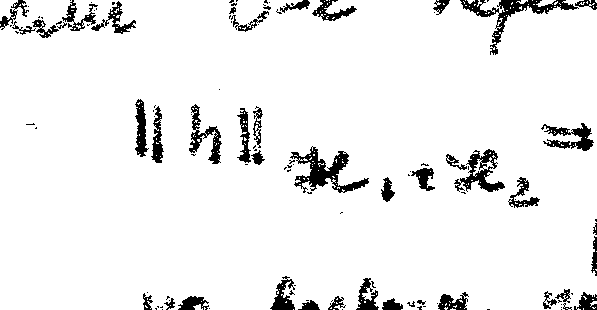
\includegraphics[width=\linewidth]{figures/gelfand-p000018-bottom-norm-part01-original-r1.png}\par\smallskip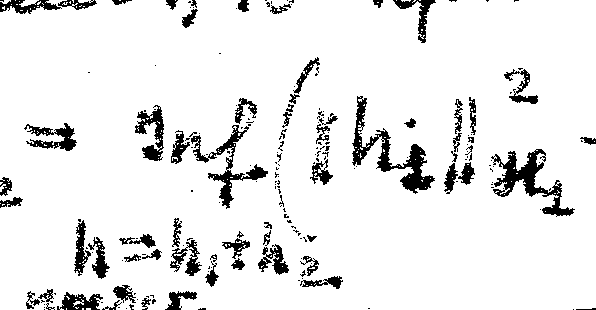
\includegraphics[width=\linewidth]{figures/gelfand-p000018-bottom-norm-part02-original-r1.png}\par\smallskip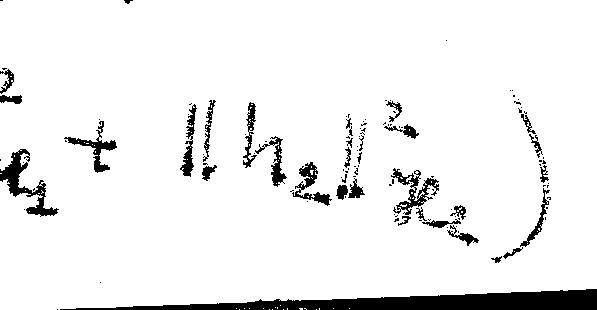
\includegraphics[width=\linewidth]{figures/gelfand-p000018-bottom-norm-part03-original-r1.png}}
\expandafter\def\csname evidence-GELFAND-P000019-diagram-01\endcsname{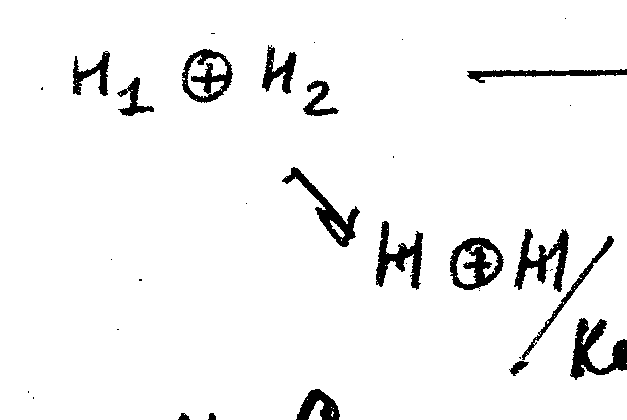
\includegraphics[width=\linewidth]{figures/gelfand-p000019-diagram-01-part01-original-r1.png}\par\smallskip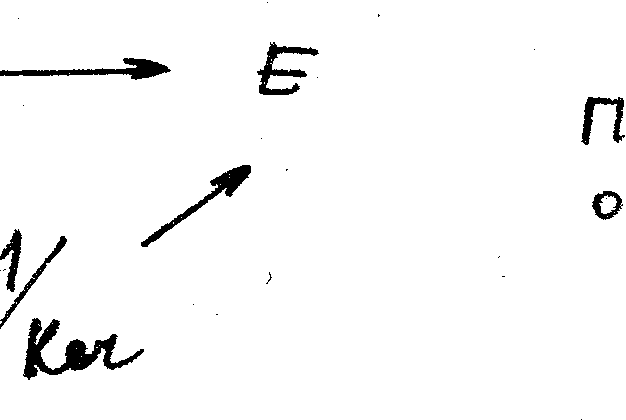
\includegraphics[width=\linewidth]{figures/gelfand-p000019-diagram-01-part02-original-r1.png}\par\smallskip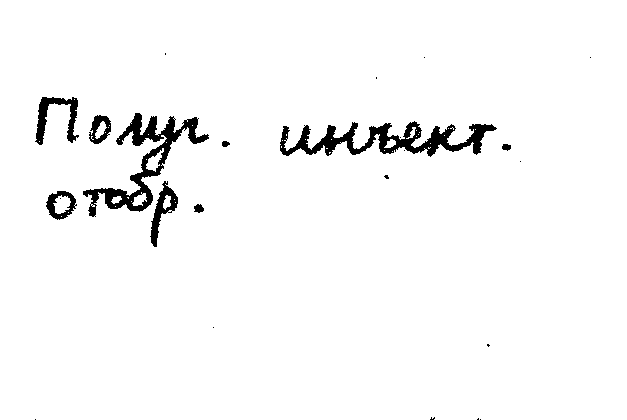
\includegraphics[width=\linewidth]{figures/gelfand-p000019-diagram-01-part03-original-r1.png}}
\expandafter\def\csname evidence-GELFAND-P000019-lower-cancellations\endcsname{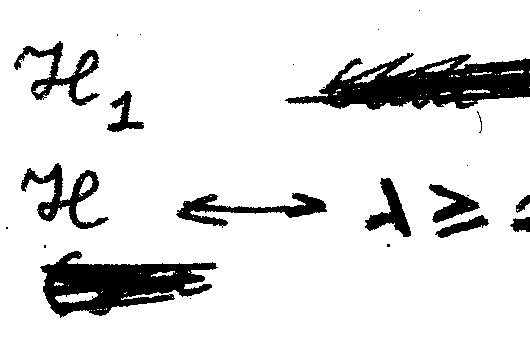
\includegraphics[width=\linewidth]{figures/gelfand-p000019-lower-cancellations-part01-original-r1.png}\par\smallskip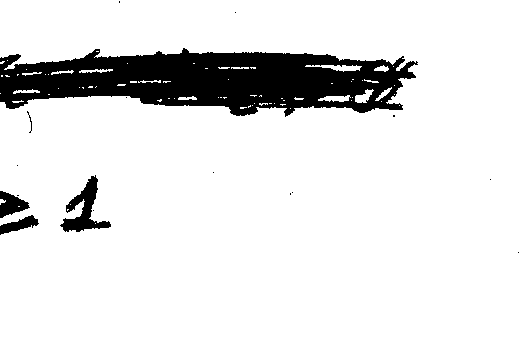
\includegraphics[width=\linewidth]{figures/gelfand-p000019-lower-cancellations-part02-original-r1.png}}
\expandafter\def\csname evidence-GELFAND-P000019-bottom-realization\endcsname{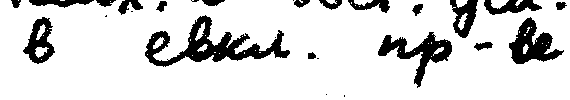
\includegraphics[width=\linewidth]{figures/gelfand-p000019-bottom-realization-part01-original-r1.png}}
\expandafter\def\csname evidence-GELFAND-P000020-middle-cancellation\endcsname{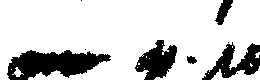
\includegraphics[width=\linewidth]{figures/gelfand-p000020-middle-cancellation-part01-original-r1.png}}
\expandafter\def\csname evidence-GELFAND-P000020-lower-example-symbol\endcsname{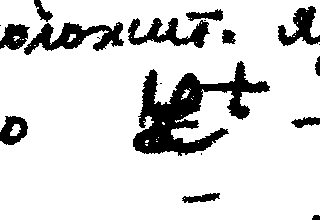
\includegraphics[width=\linewidth]{figures/gelfand-p000020-lower-example-symbol-part01-original-r1.png}}
\expandafter\def\csname evidence-GELFAND-P000017-middle-boundary-strokes\endcsname{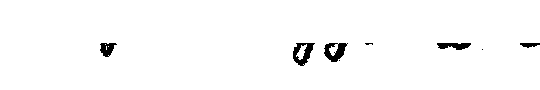
\includegraphics[width=\linewidth]{figures/gelfand-p000017-middle-boundary-left-original-r1.png}\par\smallskip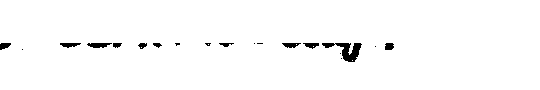
\includegraphics[width=\linewidth]{figures/gelfand-p000017-middle-boundary-right-original-r1.png}}
\begin{document}
{\large\bfseries Семинар Гельфанда — глава 1}\par
{\small Начало читательского издания. Исходные страницы 1–20. Текст и формулы набраны; каждое сомнительное чтение сопровождается исходным фрагментом. Рабочий отрывок; полная глава готовится.}\par\medskip
\SourcePage{GELFAND-P000001}{unlabelled}
Понед. $21/\mathrm{IX}$.
Декартовы и булевы произв. групп.

«Хиронака: о разрешении особенностей».
\underline{Гельфанд}

$A$ — кольцо, $\mathcal{J}$ — модуль над $A$.
\Unclear{GELFAND-P000001}{module-letter}{Буква модуля и идеала передана как $\mathcal{J}$; возможны $\mathcal{I}$ или $J$.}

Раздутие — ?
$M$ — мн.; $D\subset M$.
[Под $D$:] подмн. с особ.

$M_0^H$ — раздутие. Blowing-up.
Прообраз $D$ есть $D'$ мн. разм. $n-1$.
$D_0$ — $(n-1)$-мерное.
\SourceFigure{GELFAND-P000001}{diagram-blowup}{Три обведённых рисунка: слева область с $D$, справа сверху область с $D'$ и подписью $M_0^H$, справа снизу область и подпись $M'_0$. Верхняя стрелка направлена влево; нижняя наклонная стрелка также влево, с подписью «непр. отобр.». Точные внутренние кривые, подписи и соединение нижней области с верхней требуют сравнения со сканом.}
\Unclear{GELFAND-P000001}{blowup-notation}{Верхний индекс у $M_0$ похож на $H$; подпись нижней области похожа на $M'_0$.}

Конструкция — Гротендик.
$A$ — кольцо, $\mathcal{J}$ — модуль.
\underline{Прим.} $A$ — кольцо ф-й;
$\mathcal{J}$ — идеал ф-й, обр. в $0$ на $D$.

Получится пучок колец и пучок модулей.
$A$ — кольцо, $\mathcal{J}$ — идеал.
Построим $X$, $O_X$ — пучок колец,
$\mathcal{J}_X$ — пучок идеалов, чтобы
\begin{gather*}
 (A,\mathcal{J})\ \longleftarrow\ (X,O_X,\mathcal{J}_X).
\end{gather*}
[Под стрелкой:] лин. отобр.

$(A,\mathcal{J})$ — пучок, порожд. $1$-м ид.

$\mathcal{J}_X$ обратим, т. е. идеал кольца:
$\exists f\in\mathcal{J}_X$ такого, что $O_Xf=\mathcal{J}_X$.
[Над формулой, стрелка к $\exists$:] образ.

(Идеал — главный, если $\mathcal{J}$ — идеал.)
Тогда многообр. нулей — $1$ ур-е.

$A$ — кольцо, $\mathcal{J}$ — идеал.
\underline{Тип. пример:} $R^2$, идеал $=0$ в нач. коорд.
\Unclear{GELFAND-P000001}{origin-example}{Следующая строка: «Вклеив. в $0$ проект. прямой»; начало может читаться «Оклеив.».}

$A$, $\mathcal{J}$ — мод.
\begin{gather*}
 \mathcal{J}\otimes_A\mathcal{J},\qquad
 \mathcal{J}\otimes_A\mathcal{J}\otimes_A\mathcal{J},\ldots
\end{gather*}
[Над группами тензорных произведений:] симм.; симм.

Рассм. форм. суммы
\begin{gather*}
 \sum_{k=0}^{N}a_kz^k.
\end{gather*}
Склад. и умн.
$x\otimes y=y\otimes x$.
\begin{gather*}
 a_0\in A,\qquad a_1\in\mathcal{J},\qquad
 a_2\in\mathcal{J}\otimes_A\mathcal{J}\quad\text{—}
\end{gather*}

\SourcePage{GELFAND-P000002}{unlabelled}
Кольцо таких сумм $S_A(\mathcal{J})$.
Рассм. однор. идеалы
[над строкой вставлено:] (градуир.).
(Вместе с многочленом сод. все его однородные.)

Рассм. все простые однор. идеалы в $S_A(\mathcal{J})$.
Выбр. идеалы, к-рые сод. все мн., нач. с $1$-й степени.
\Unclear{GELFAND-P000002}{ideal-selection}{Конец строки после «сод. все» лучше читается как «мн., нач. с $1$-й степени»; средние штрихи сокращения «нач.» остаются не вполне различимыми.}

Совок. идеалов $X$. (Топология Зарисского.)
$O_X$, $\mathcal{J}_X$.
Если $U$ откр. мн-во, то $O_U$, $\mathcal{J}_U$.
\Unclear{GELFAND-P000002}{open-set-notation}{После «то» первая буква совпадает по форме с $O_X$ выше, вторая — с буквой идеала: $O_U$, $\mathcal{J}_U$; последняя может быть $\mathcal{I}_U$.}

$S_A(\mathcal{J})$ — всё кольцо.
Кольцо отношений, числ., знамен., не прин. ни одному из идеалов.
Локализ. кольцо на это мн-во.
Отнош. $1$-й степени $\mathcal{J}_U$.
\Unclear{GELFAND-P000002}{fractions-sentence}{В строке об отношениях не вполне ясны сокращения «числ.-знамен.» и то, относится ли «не прин.» только к знаменателю. Слова не дополнены по смыслу.}
[Справа, две стрелки вниз:] Гротендик — раздуть идеально.
\Unclear{GELFAND-P000002}{margin-grothendieck}{Правая помета читается как «Гротендик — раздуть идеально»; последнее слово возможно «идеально» или «идеалы».}

$A$ — кольцо многочл. $2$-х пер.
$\mathcal{J}$ — идеал из мн. $P(0,0)=0$.
\begin{gather*}
 A=\{P(x,y)\},\qquad
 \mathcal{J}=P(x,y)=a_1x+b_1y+\cdots .
\end{gather*}
\begin{gather*}
 \mathcal{J}\otimes_A\mathcal{J}\ \longleftrightarrow
 \{a_2x^2+2b_2xy+cy^2+\cdots\}.
\end{gather*}
\Unclear{GELFAND-P000002}{quadratic-coefficients}{Коэффициенты в квадратном многочлене читаются $a_2$, $2b_2$, $c$; индекс у $c$ и вид толстой двусторонней стрелки не уверены.}

Из-за переброски получ. то же, что квадрат идеала.
Тогда — идеал из мн., равных $0$ в этой точке.
Во что она раздуется? ?

\begin{gather*}
 \sum P_k(x,y)z^k,\qquad P_k(x,y)=ax^k+\cdots .
\end{gather*}
[Справа:] Градуир. $\Sigma$ тенз. произвед.
\begin{gather*}
 A=\{P_0(x,y)\}\longrightarrow S_A(\mathcal{J}),\qquad
 P_0(x,y)\sim P_0(x,y).
\end{gather*}
Набор простых идеалов, получ. из ид. $P(0,0)=0$.
\begin{gather*}
 S_A\sim\sum P_kz^k,\qquad P_k\in\mathcal{J}^k,\qquad
 K\sim\sum P_kz^k.
\end{gather*}
Дост. найти max ид. факторкольца —
(чтобы найти ид., сод. данный).
\begin{gather*}
 S_A/K\ \longleftrightarrow\ a_0+(a_1x-b_1y)z+\cdots .
\end{gather*}
\Unclear{GELFAND-P000002}{last-sign}{В последней формуле перед $b_1y$ виден минус, хотя на следующем скане стоит плюс. Сохранён видимый минус; направление толстой стрелки также не вполне ясно.}

\SourcePage{GELFAND-P000003}{2}
Все однор. max ид. в нём и будут точками расширения.
Своб. члена нет (тогда и $1$).
\begin{gather*}
 (a_1x+b_1y)z.
\end{gather*}
Только $1$ лин. комб. $x$ и $y$.
($2$ нет, т. к. тогда все.)

Идеалы опр. напр. на плоскости
(замк. всеми возм. напр. — $\sigma$-процесс).
\Unclear{GELFAND-P000003}{directions}{Сокращения в скобках читаются «замк. всеми возм. напр.»; первое слово и значение знака $\sigma$ не утверждаются.}
\Needspace{48mm}\underline{Задача.} В пр-ве
[зачёркнуто:] \Unclear{GELFAND-P000003}{cross-cancellation}{Зачёркнутое слово перед рисунком не читается.}
\par\smallskip\noindent\begin{minipage}{\linewidth}\begin{minipage}[t]{.47\linewidth}\centering\vspace{0pt}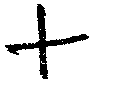
\includegraphics[width=30mm]{figures/gelfand-p000003-cross-diagram-original-r1.png}\par{\scriptsize Исходный рисунок}\end{minipage}\hfill\begin{minipage}[t]{.49\linewidth}\centering\vspace{0pt}\begin{tikzpicture}[scale=0.5]
 \draw (-0.8,0)--(0.8,0);
 \draw (0,-0.7)--(0,0.8);
\end{tikzpicture}\par{\scriptsize Наборное воспроизведение}\end{minipage}\end{minipage}\par\smallskip
Что получ. при заклеивании?
\begin{gather*}
 z=0,\qquad xy=0,\qquad \mathcal{J}=(z,xy).
\end{gather*}
[Под системой проведена черта.]

\underline{Добрушин.}
[Зачёркнуто перед «Найти»:] \Unclear{GELFAND-P000003}{ising-cancellation}{Зачёркнутое начало строки не читается уверенно.}
Найти пример газа, в к-ром сущ. фаз. переходы.
Куб целочисл. решётки.
$\ell$ — длина. $V_\ell=\ell^\nu$.
$N$ точ. $N<V_\ell$.
Могут заним. полож. на решётке
$\theta=(x_1,\ldots,x_N)$.
\Unclear{GELFAND-P000003}{configuration-letter}{Знак конфигурации передан как $\theta$; рукописный знак также похож на $b$ или кириллическое «в».}

Модель Изинга.
[Перед формулой густой зачёркнутый знак:]
\Unclear{GELFAND-P000003}{energy-cancellation}{Отдельный зачёркнутый знак перед $U(\theta)$ не читается.}
\begin{gather*}
 U(\theta)=-\frac12\sum_{i\ne j}u(x_i,x_j),\qquad
 u=\begin{cases}
 0&\text{в ост. случ.},\\
 1;&\rho(x_i,x_j)=1.
 \end{cases}
\end{gather*}
$u(\theta)$ — число пар соседних точек.
\Unclear{GELFAND-P000003}{energy-case}{В условии второй ветви виден знак, похожий на $\rho$; точка с запятой после $1$ сохранена. В подписи ниже первая буква похожа на малое $u$, а не $U$.}

Осн. аксиом — распр. Гиббса.
\begin{gather*}
 \mathsf{P}(B)=
 \frac{\displaystyle\sum_{\theta\in B}\exp\{-U(\theta)/T\}}
 {Z(V_\ell,N)},\qquad T>0\text{ — темпер.}
\end{gather*}
[Под знаменателем:] норм. множ.
\begin{gather*}
 Z(\ell,N)=\sum_{\theta\in\mathcal{B}}\exp\{-U(\theta)/T\}.
\end{gather*}
\Unclear{GELFAND-P000003}{partition-domain}{В знаменателе первой формулы написано $Z(V_\ell,N)$, следующая строка — $Z(\ell,N)$; знак множества под суммой похож на $\mathcal{B}$. Не исправлено по согласованности.}

Молекулы притяг.
([Два закрашенных знака со стрелками:] соседи $>$ их вероятн.)
\Unclear{GELFAND-P000003}{attraction-note}{В скобках после «Молекулы притяг.» закрашенные знаки и стрелки; чтение «соседи $>$ их вероятн.» не уверено.}
$B\subset\mathcal{B}$ — совок. распол.
\begin{gather*}
 p(\theta)=\frac{\exp\{-U(\theta)/T\}}{Z(\ell,N)}.
\end{gather*}
Пред. перех. $\ell\to\infty$, куб раздув. до $\infty$.
$N_\ell$ зав. от $\ell$.
[Зачёркнутый знак перед дробью:]
\Unclear{GELFAND-P000003}{density-cancellation}{Зачёркнутый знак перед $V_\ell/N_\ell$ не читается.}
\begin{gather*}
 \frac{V_\ell}{N_\ell}=v=\mathrm{const}.
\end{gather*}
Реш. увеличивается.
Можно показ., что
\begin{gather*}
 \frac1{N_\ell}\log Z(\ell,N_\ell)\longrightarrow f(v,T).
\end{gather*}

\SourcePage{GELFAND-P000004}{unlabelled}
\begin{gather*}
 p(v,T)=T\frac{\partial f}{\partial v}\qquad\text{по опред.}
\end{gather*}
\Unclear{GELFAND-P000004}{pressure-letter}{В первом аргументе $p$ густой знак похож на $v$; перед производной минус не виден и не добавлен.}

Фаз. переход.
По поводу $f$ — это монот., выпуклая ф-я по $v$.
Поэтому $p>0$ и $p$ монот. ф-я $v$.
Фаз. переход: $p(v,T)$ им. плоский участок.
\SourceFigure{GELFAND-P000004}{diagram-phase-point}{В правом верхнем поле ломаная S-подобная кривая с почти горизонтальным средним отрезком и стрелкой к нему; подпись «точки фаз. перехода». Точные оси и точки на исходном рисунке не обозначены уверенно.\par\smallskip\centering\resizebox{.93\linewidth}{!}{\begin{tikzpicture}[x=1cm,y=1cm]
\draw[thick] (0,0)..controls(.25,.2)and(.25,.85)..(.55,.9)--(2.25,.9)..controls(2.7,.9)and(2.55,1.4)..(2.8,1.8);
\fill(1.35,.9)circle(1.8pt);
\draw[thick](1.35,.87)..controls(1.35,.47)and(1.5,.45)..(1.9,.45);
\node[anchor=west,align=left,font=\small]at(2.15,.25){\PhaseWords};
\end{tikzpicture}}\par{\scriptsize Наборная схема; ограничения указаны в примечании.}\par}
Есть физич. гипотеза — $1$ уч. перех.

\SourceFigure{GELFAND-P000004}{diagram-cancelled-graph}{Слева график с вертикальной и горизонтальной осями, $0$ и $\infty$ у горизонтальной оси. Несколько кривых и прямых густо перечёркнуты; точная зачёркнутая кривая и вертикальная подпись требуют проверки.\par\smallskip\centering\resizebox{.93\linewidth}{!}{\begin{tikzpicture}[x=1cm,y=1cm]
\draw[thick](0,1.75)--(0,0)--(3.6,0);
\node[below]at(0,-.05){$0$};\node[below]at(3.6,-.05){$\infty$};
\end{tikzpicture}}\par{\scriptsize Частичное воспроизведение: только уверенные оси; зачёркнутые кривые не восстановлены.}\par}
\SourceFigure{GELFAND-P000004}{diagram-pressure-plateau}{Соседний рисунок справа: чистая убывающая кривая с плоским участком. Это отдельный график, а не восстановление зачёркнутого рисунка слева.\par\smallskip\centering\resizebox{.9\linewidth}{!}{\begin{tikzpicture}[scale=0.7]
 \draw (0,0)--(4.6,0);
 \draw (0,0)--(0,2.3);
 \draw (0.2,2.5).. controls (0.9,2.4) and (0.5,1.25)..(1.2,1.15)
 --(2.4,1.15).. controls (2.9,1.05) and (2.7,0.45)..(4,0.35);
 \node at (-0.1,-0.4) {$0$};
 \node at (4.6,-0.4) {$\infty$};
\end{tikzpicture}}\par{\scriptsize Прежнее наборное воспроизведение.}}
Плоский отр. есть при дост. малых $T$ ($<T_{\text{крит}}$).

Допускает явное реш. при $n=1$.
Считается $Z$ и $f(v,T)$.
Фаз. переходов нет, что счит. физич. естественным.

\underline{$n=2$.} \underline{Онзагер.}
$f(v,T)$ выч. для частных $v$ и $T$.
Разрыв производной соотв. фаз. переходам.
\SourceFigure{GELFAND-P000004}{diagram-onsager}{График с осью $T$ вверх, осью $v$ вправо, подписью $1/2$ под вертикалью через вершину. Кривая поднимается слева к вершине, убывает вправо; вертикальная линия проходит через вершину, справа от неё небольшой волнистый отрезок. Точная геометрия и значение волнистой ветви не установлены.\par\smallskip\centering\resizebox{.93\linewidth}{!}{\begin{tikzpicture}[x=1cm,y=1cm]
\draw(0,0)--(4.6,0);\draw(0,0)--(0,2.3);
\node[left]at(0,2.3){$T$};\node[below]at(4.6,0){$v$};
\draw(2.2,-.05)--(2.2,2.65);\node[below]at(2.2,-.12){$1/2$};
\draw[thick](.7,-.02)..controls(1.25,.35)and(1.85,.95)..(2.2,1.35)..controls(2.4,1.1)and(3.05,.55)..(3.45,.18);
\draw(1.05,.18)..controls(1.5,.54)and(1.9,1)..(2.17,1.35);
\fill(2.2,1.35)circle(1.5pt);
\draw[thick](2.32,1.4)..controls(2.5,1.62)and(2.63,1.33)..(2.78,1.42)..controls(2.86,1.47)and(2.98,1.56)..(3.03,1.61);
\end{tikzpicture}}\par{\scriptsize Наборная схема; ограничения указаны в примечании.}\par}

Kac, Helfand.
Точн. в яв. виду для нек-рых случаях.
\Unclear{GELFAND-P000004}{kac-helfand-note}{После повторного увеличения строка читается «точн. в яв. виду для нек-рых случаях»; возможны окончания «виде» и «случаев». Неграмматичное чтение не заменено автоматически.}

\SourceFigure{GELFAND-P000004}{diagram-subcube}{Большой квадрат и меньшая обведённая область внутри; в центре $H$, над малой областью $h$. Малый контур отчасти квадратный, отчасти округлый; точные границы не восстановлены.\par\smallskip\centering\resizebox{.93\linewidth}{!}{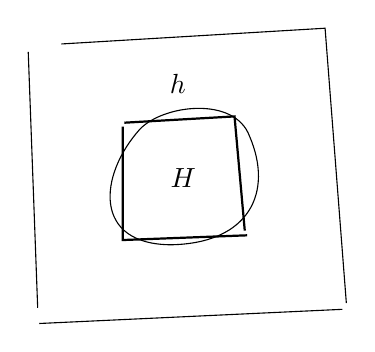
\begin{tikzpicture}[x=1cm,y=1cm]
\draw(.3,3.45)--(3.65,3.65)--(3.92,.16);\draw(3.87,.08)--(.02,-.1);\draw(0,.1)--(-.12,3.35);
\draw[thick](1.1,2.45)--(2.5,2.53)--(2.63,1.08);\draw[thick](2.66,1.02)--(1.08,.96)--(1.08,2.4);
\draw(1.3,2.37)..controls(1.6,2.68)and(2.5,2.79)..(2.69,2.28)..controls(3,1.56)and(2.68,.92)..(1.7,.9)..controls(.7,.9)and(.77,1.78)..(1.3,2.37);
\node at(1.85,1.75){$H$};\node at(1.78,2.94){$h$};
\end{tikzpicture}}\par{\scriptsize Наборная схема; ограничения указаны в примечании.}\par}
\begin{gather*}
 \frac{\mu_H}{h^\nu}.
\end{gather*}
$\mu_H$ — число частиц в $H$ — подкуб.
$\nu$ — размерность.
\begin{gather*}
 \frac{\mu_H}{h^\nu}=\frac1v\qquad\text{как и во всём пр-ве.}
\end{gather*}
\underline{Зак. больших чисел.}
\begin{gather*}
 \mathsf{P}\left\{\frac{\mu_H}{h^\nu}-\frac1v\,\middle|\,>\varepsilon\right\}
 \longrightarrow0.
\end{gather*}
\Unclear{GELFAND-P000004}{probability-bar}{В вероятностной формуле правая вертикальная черта перед $>\varepsilon$ видна, левая черта перед дробью не прочитана уверенно. Формула не дополнена молча парной чертой.}
\begin{gather*}
 \ell\to\infty,\qquad H\to\infty,\qquad
 d<\frac h\ell<1-d,\qquad d>0.
\end{gather*}
\Unclear{GELFAND-P000004}{bottom-mark}{У нижнего правого края небольшой знак похож на «2» или оборванную букву; как номер страницы не принят.}
\Incomplete{GELFAND-P000004}{margin-left}{Вдоль самого левого края видна узкая полоса соседнего рукописного текста, обрезанная до отдельных окончаний и штрихов; связный текст не читается.}



\SourcePage{GELFAND-P000005}{3}
Если это \underline{не} вып., то имеет место фазовый переход.
\Unclear{GELFAND-P000005}{physical-meaning-heading}{Нагл. [кандидат сокращения; средние штрихи не вполне различимы]} смысл. Сосущ. $2$ фазы, част. расп. неравномерно —
— жидкость и газ.
[Над строкой:] (зак. больш. чисел).
[Вставка над «фаз. перехода», со скобкой:] отсутствия.
(Близкое усл. необх. и дост. для фаз. перехода
\begin{gather*}
 \mathsf{P}_\ell\left\{\left|\frac{\mu_H}{h^\nu}-\frac1v\right|>\varepsilon\right\}
 =O(e^{-N\beta}).
\end{gather*}
\Unclear{GELFAND-P000005}{exponential-rate}{Показатель у $e$ содержит густо записанный знак перед $\beta$; кандидат $-N\beta$, но $N$ закрыт наложенными штрихами. Скобка, открытая перед «Близкое», на скане явно не закрыта.}
[Справа:] $N$ — число частиц.

Подсчит. вер., что
\begin{gather*}
 \mathsf{P}\{\mu_H=k\}=Z^{-1}
 \sum_{\theta\in\mathcal{B}_k}\exp\{-U(\theta)/T\}.
\end{gather*}
По распол., в к-рых в $H$ сидят $k$ частиц.
$\theta$ — распол. $N$ частиц.
$\theta\in\mathcal{B}_k$.
Тогда $\theta=(\theta_1,\theta_2)$.
$\theta_1$ расп. $k$ частиц в $H$.
$\theta_2$ расп. $(N-k)$ частиц в $\overline H$.
\Unclear{GELFAND-P000005}{complement-label}{У $H$ в строке про $\theta_2$ верхняя черта не вполне отчётлива; кандидат $\overline H$.}
\begin{gather*}
 U(\theta)=U(\theta_1)+U(\theta_2)+\gamma(\theta).
\end{gather*}
$U(\theta_1)$ — взаимод. внутри.
$U(\theta_2)$ — соседи вне.
$\gamma(\theta)$ — взаимод. через пов.
$\gamma(\theta)$ можно асимптотически пренебречь.
(Через гран. — пор. числа гран. точек)
$V^{\nu-1/\nu}$ при $N\to\infty$.
$k\sim dN$.
\Unclear{GELFAND-P000005}{boundary-exponent}{Степень у $V$ выглядит как $\nu-1/\nu$, без уверенно различимого общего числителя. Не заменена автоматически на $(\nu-1)/\nu$.}
\begin{gather*}
 |\gamma(\theta)|\le CN^{\frac{\nu-1}{\nu}}.
\end{gather*}
\begin{align*}
 \sum\exp\{-U(\theta)/T\}
 &=\sum_{\theta\in\mathcal{B}_k}\exp\{-U(\theta_1)/T\}
 \exp\{-U(\theta_2)/T\}\\
 &\qquad\times
 \exp\{\theta N^{2/3}\}
 =
\end{align*}
\Unclear{GELFAND-P000005}{theta-factor}{Буква перед $N^{2/3}$ похожа на $\theta$ или $\Theta$; на скане та же буква ниже пояснена «огранич. параметр». Она может отличаться от знака конфигурации.}
$\theta$ — огранич. параметр.
\begin{gather*}
 =\exp\{\theta N^{2/3}\}
 \sum_{\theta_1}\exp\{-U(\theta_1)/T\}
 \sum_{\theta_2}\exp\{-U(\theta_2)/T\}.
\end{gather*}
[Под первой суммой:] распол.



\SourcePage{GELFAND-P000006}{unlabelled}
$1$-й сомнож.: $Z$, выч. для подкуба.
$2$-й — » — $Z$ для внешн. куба.
\begin{gather*}
 \mathsf{P}\{\mu_H=k\}
 =\frac{Z(H,k)Z(\overline H,N-k)}{Z(V,N)}
 \exp\{\theta N^{2/3}\}.
\end{gather*}
[Звёздочка.]
К ним прим. асимпт. ф-лу
\begin{gather*}
 Z(V,N)\approx\exp\{-Nf(v,T)\},
\end{gather*}
\begin{gather*}
 Z(H,k)=\exp\{-kf(h^3/k,T)\}.
\end{gather*}
\Unclear{GELFAND-P000006}{subcube-power}{В числителе аргумента $f$ в этой строке видна степень $3$ у $h$, хотя дальше употребляется $\nu$. Сохранено $h^3$.}
Можно док. и для хор. обл. (не куба).
Пред. ф-ла не зав. от формы области.
\begin{gather*}
 Z(\overline H,N-k)=
 \exp\{-(N-k)f((\ell^3-h^3)/(N-k),T)\}.
\end{gather*}
Подставить туда в предп., что $f$ им. лин. участок.
Если $f$ им. лин. участок (у произв. горизонт.),
тогда сокр. и получим
\begin{gather*}
 \frac1N\log\mathsf{P}\{\mu_H=k\rho\}\longrightarrow
 \begin{cases}
 0&\text{лишь при }\rho=1/v\text{ (если лин. уч. нет)},\\
 0&\rho\in\text{ лин. участку}.
 \end{cases}
\end{gather*}
[Зачёркнуто у второй ветви:]
\Unclear{GELFAND-P000006}{limit-notation}{Аргумент события выглядит $\mu_H=k\rho$, но последний знак может быть $\theta$ или $\delta$. Буква плотности справа похожа на $\rho$. Зачёркнутый текст над второй ветвью не прочитан.}
\SourceFigure{GELFAND-P000006}{diagram-limit-step}{Справа от второй ветви предела небольшой штрих: снизу слева линия поднимается почти вертикально, затем идёт вправо почти горизонтально, после чего на правом конце вновь поднимается вверх. Отдельные оси, стрелки и подписи у этой схемы не установлены; её математическое значение требует исходного изображения.\par\smallskip\centering\resizebox{.93\linewidth}{!}{\begin{tikzpicture}[x=1cm,y=1cm]
\draw[thick] (0,0)..controls(.2,.65)and(.35,1.2)..(.65,1.35)--(2.4,1.4)--(2.45,2.15);
\end{tikzpicture}}\par{\scriptsize Видимый штрих; оси и значения не добавлены.}\par}
$\mathsf{P}\to0$ exp образом.
($1/v$ получ. из \underline{выпуклости} $f$.)

Располож. частиц.
Его граница; вокруг каждой кубик со стор. $1$.
$\Gamma'(\theta)$ — граница занятой области.
$\Gamma(\theta)$ — длина
[вставлено снизу:] площадь.
\SourceFigure{GELFAND-P000006}{diagram-cell-clusters}{В квадратной рамке слева вертикальная заштрихованная цепочка; внутренние разделения сливаются со штриховкой. Справа три клетки углом: две внизу и одна над левой. Число клеток слева не установлено.\par\smallskip\centering\resizebox{.93\linewidth}{!}{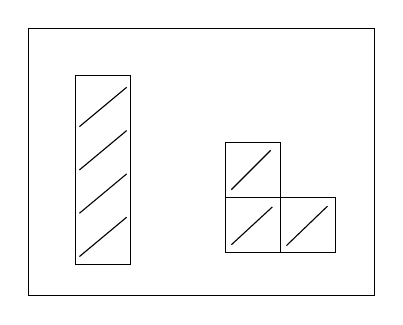
\begin{tikzpicture}[x=1cm,y=1cm]
\draw(0,0)rectangle(4.4,3.4);
\draw(.6,.4)rectangle(1.3,2.8);
\draw(2.5,.55)rectangle(3.2,1.25);\draw(3.2,.55)rectangle(3.9,1.25);\draw(2.5,1.25)rectangle(3.2,1.95);
\foreach \y in{.5,1.05,1.6,2.15}{\draw(.65,\y)--(1.25,\y+.5);}
\draw(2.58,.65)--(3.1,1.13);\draw(3.28,.64)--(3.8,1.14);\draw(2.58,1.35)--(3.08,1.85);
\end{tikzpicture}}\par{\scriptsize Частичная схема левой цепочки; внутреннее деление не установлено. Справа три клетки углом.}\par}
\underline{Замен.} Гиббсов. вер.
\begin{gather*}
 \mathsf{P}(\theta)=
 \frac{\exp\{-U(\theta)/T\}}{\sum\exp\{-U(\theta)/T\}}
 =\frac{\exp\{-\Gamma'(\theta)/(2T)\}}
 {\sum\exp\{-\Gamma'(\theta)/(2T)\}}.
\end{gather*}
\Unclear{GELFAND-P000006}{gamma-prime}{Штрих у $\Gamma$ в двух показателях после равенства не вполне ясен; видимая буква похожа на $\Gamma'$ или $\Gamma$.}
[Справа:] $2\nu-\delta$.
Незанятые \underline{квадратики} $\Gamma'(\theta)$.
[Вставлено:] у соседей.
\begin{gather*}
 -U(\theta)\ \ge\ \sum(2\nu-\delta)
 =2\nu N-\sum_{\Gamma'(\theta)}\delta.
\end{gather*}
\Unclear{GELFAND-P000006}{energy-bound}{Знак после $-U(\theta)$ написан поверх другого: кандидаты $\ge$, $\le$, $=$. Знак перед суммой в самом конце и индекс суммы могут относиться к другому члену; сохранён видимый кандидат без исправления по математике.}



\SourcePage{GELFAND-P000007}{4}
($U(\theta)$ — минус число соседей.)
Меньше граница — более выгодно расположение.
Загнать в один угол, но это невыгодно
(всего таких расп. мало).
Конечное число клубков.
(Внутри газа — жидкость.)
\SourceFigure{GELFAND-P000007}{diagram-small-clusters}{Малый квадратный рисунок справа: две закрашенные области и маленькие штрихи в верхнем левом углу. Число и смысл мелких штрихов не ясны.\par\smallskip\centering\resizebox{.93\linewidth}{!}{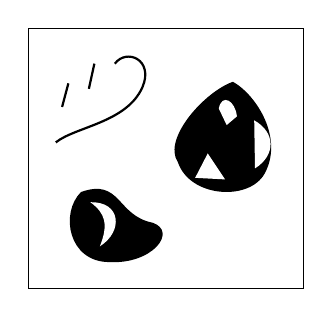
\begin{tikzpicture}[x=1cm,y=1cm]
\draw(0,0)rectangle(3.5,3.3);
\draw[thick](.35,1.85)..controls(.6,2.05)and(1.25,2.1)..(1.45,2.55)..controls(1.6,2.9)and(1.25,3.05)..(1.1,2.85);
\draw[thick](.43,2.3)--(.51,2.6);\draw[thick](.77,2.53)--(.84,2.85);
\fill(2.6,2.62)..controls(2.9,2.45)and(3.25,1.9)..(3,1.45)..controls(2.8,1.1)and(2.05,1.15)..(1.9,1.6)..controls(1.7,1.9)and(2.25,2.5)..(2.6,2.62);
\fill[white](2.42,2.28)..controls(2.46,2.48)and(2.63,2.38)..(2.65,2.18)--(2.52,2.07)--cycle;
\fill[white](2.87,2.13)..controls(3.14,1.98)and(3.15,1.69)..(2.88,1.52)--cycle;
\fill[white](2.28,1.71)--(2.5,1.38)--(2.12,1.4)--cycle;
\fill(.67,1.22)..controls(1.18,1.4)and(1.12,.92)..(1.58,.83)..controls(1.9,.72)and(1.58,.3)..(1.03,.33)..controls(.51,.33)and(.4,.95)..(.67,1.22);
\fill[white](.79,1.09)..controls(1.18,1.1)and(1.21,.72)..(.91,.53)..controls(1.02,.81)and(.98,.95)..(.79,1.09);
\end{tikzpicture}}\par{\scriptsize Частичная схема пятен и видимых отметок; мелкие штрихи не истолкованы.}\par}
И это противоречит закону больших чисел.

\SourceFigure{GELFAND-P000007}{diagram-cycles}{Большая прямоугольная рамка слева, внутри три отдельные округлые области с внутренними контурами и заштрихованными участками, одна имеет центральный островок. Точные циклы, штриховка и вложенность требуют исходного изображения.\par\smallskip\centering\resizebox{.93\linewidth}{!}{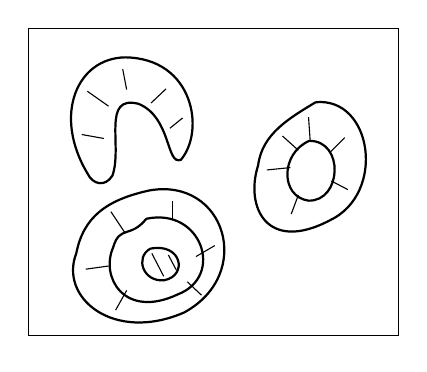
\begin{tikzpicture}[x=1cm,y=1cm]
\draw(0,0)rectangle(4.7,3.9);
\draw[thick](.75,2.06)..controls(.31,2.8)and(.62,3.52)..(1.23,3.53)..controls(2.1,3.52)and(2.25,2.6)..(1.94,2.23)..controls(1.75,2.15)and(1.82,2.77)..(1.4,2.94)..controls(.93,3.06)and(1.2,2.4)..(1.07,2.03)..controls(.98,1.88)and(.82,1.91)..(.75,2.06);
\draw(.68,2.55)--(.96,2.5);\draw(.75,3.1)--(1.02,2.91);\draw(1.2,3.38)--(1.25,3.12);\draw(1.75,3.13)--(1.56,2.95);\draw(1.96,2.76)--(1.8,2.63);
\draw[thick](3.65,2.96)..controls(4.37,3.03)and(4.55,1.8)..(3.83,1.46)..controls(3.03,1.04)and(2.75,1.63)..(2.92,2.16)..controls(2.97,2.56)and(3.32,2.76)..(3.65,2.96);
\draw[thick](3.57,2.47)..controls(4.02,2.47)and(3.98,1.7)..(3.56,1.71)..controls(3.2,1.76)and(3.2,2.31)..(3.57,2.47);
\draw(3.03,2.1)--(3.33,2.13);\draw(3.23,2.53)--(3.43,2.35);\draw(3.56,2.77)--(3.58,2.48);\draw(4.02,2.51)--(3.84,2.33);\draw(4.06,1.85)--(3.85,1.96);\draw(3.34,1.54)--(3.43,1.78);
\draw[thick](1.54,1.84)..controls(2.5,2.01)and(2.88,.78)..(1.98,.29)..controls(1.08,-.1)and(.39,.48)..(.61,1.04)..controls(.7,1.5)and(.99,1.72)..(1.54,1.84);
\draw[thick](1.5,1.48)..controls(2.2,1.63)and(2.5,.75)..(1.9,.52)..controls(1.22,.2)and(.91,.74)..(1.08,1.12)..controls(1.16,1.4)and(1.3,1.23)..(1.5,1.48);
\draw[thick](1.55,1.1)..controls(1.95,1.18)and(2.03,.76)..(1.73,.7)..controls(1.46,.67)and(1.35,.99)..(1.55,1.1);
\draw(1.57,1.04)--(1.72,.75);\draw(1.78,1.02)--(1.88,.83);
\draw(.73,.84)--(1.02,.88);\draw(1.05,1.57)--(1.23,1.3);\draw(1.83,1.7)--(1.83,1.48);\draw(2.37,1.14)--(2.13,1);\draw(2.2,.51)--(2.02,.68);\draw(1.11,.32)--(1.25,.57);
\end{tikzpicture}}\par{\scriptsize Схема вложенности с открытым нижним промежутком в верхней левой группе.}\par}
Вся граница распад. на связные циклы.
У каждого расп. своё число.
Занумер. их
\begin{gather*}
 \Gamma_1(\theta)\ge\Gamma_2(\theta)\ge\cdots,\qquad
 \Gamma(\theta)=\sum_i\Gamma_i(\theta).
\end{gather*}
Расп. особое, если $\exists N<\infty$, $D<\infty$, $\delta>0$.
\Unclear{GELFAND-P000007}{special-arrangement-count}{В этой строке первый конечный параметр похож на $N$, а в последующих суммах предел похож на $M$. Различие не сглажено.}
\begin{gather*}
 1)\quad\sum_{i=1}^{M}\Gamma_i(\theta)
 \le D\ell^{\frac{\nu-1}{\nu}}.
\end{gather*}
[Под суммой:] Большие.
Пор. длины границы. (Почти весь куб.)
\Unclear{GELFAND-P000007}{large-cycles-power}{Степень у $\ell$ в первом условии записана дробью, читается $(\nu-1)/\nu$; на скане GELFAND-P000010 аналогичная строка имеет $\nu-1$. Оставлено различие.}
\begin{gather*}
 2)\quad\text{все ост. маленькие}\qquad
 \sum_{i=1}^{M}\bigl(\Gamma_i(\theta)\bigr)^{\frac\nu{\nu-1}}.
\end{gather*}
\Unclear{GELFAND-P000007}{small-cycles-sum}{Видимые пределы второй суммы выглядят $1$ и $M$, хотя подпись говорит «все ост. маленькие». После суммы условия не видно; оно не дописано по следующему скану.}
[Разделительная черта.]

$24/\mathrm{IX}$.
Четверг. $16$ ч. ауд. $13$-$11$.
Проф. Сигал (USA).
\underline{Теория ф-й в беск.-мерном пр-ве.}
\begin{gather*}
 +\Box\varphi=m^2\varphi+g\varphi^3.
\end{gather*}
\begin{gather*}
 F_f(\varphi)=\int(-\Box+m^2)f\varphi
 +g\int\varphi^3 f.
\end{gather*}
[Над $\varphi^3$:] $\varphi$ — мн.
$\varphi$ [стрелка] $C_0^\infty$ — ф-и.
\Unclear{GELFAND-P000007}{field-margin}{Над правой пометой видны «б, ф-й на» и стрелка к $C_0^\infty$; возможно это определение функции $\varphi$ на пространстве пробных функций, но текст не дополнен.}
$g$ — фикс.
$F_f\in\Phi$ — нелин. ф-л от $\varphi$.
$\Phi$ — кольцо; можно умн. $F_1(\varphi)F_2(\varphi)$.
Берём идеал, порожд. $(F_f:f\in C_0^\infty)$ — $\Omega$.
\Unclear{GELFAND-P000007}{ideal-signature}{Индекс у $F$ в определении идеала похож на $f$; исходный знак после скобки — $\Omega$ или каллиграфическое $J$.}
Пусть $p=\Phi/\Omega$ — функц. кольцо на многообр. реш.
зад. ур-я в частн. произв.
Чтобы получить реш. $(1)$ $\overset{\mathrm{def}}=$
точка пр-ва max идеалов кольца $p$.
Обычн. реш. $\varphi_0$ [галочка над словом] — сопост. max идеал — рассм. отобр.
\begin{gather*}
 F\longrightarrow F(\varphi_0),
\end{gather*}
гомоморфизм в $\Phi$,
$F_f$ нулевой на идеале $\Omega$.
Это гом. и факторкольца, т. е. max идеал.
\Unclear{GELFAND-P000007}{evaluation-target}{После «гомоморфизм в» видимая буква похожа на $\Phi$, хотя по смыслу могло быть поле. Сохранён буквенный кандидат, а не математическое исправление.}



\SourcePage{GELFAND-P000008}{unlabelled}
Max идеал — обобщ. реш. нелин. ур-я.
Алг. случай.
\begin{gather*}
 f_1(x_1,\ldots,x_n)=0,\qquad
 f_k(x_1,\ldots,x_n)=0.
\end{gather*}
Реш. в терминах кольца — в кольце всех мн.
Идеал, порожд. этими ф-ями $p$, и факторкольцо
$\Phi/p$.
\Unclear{GELFAND-P000008}{algebra-ring-letter}{В дроби числитель похож на $\Phi$, $P$ или густо написанное $A$; сохранён кандидат $\Phi$.}
$\Phi$ — все ур-я.
Это кольцо алг. ф-и.
Точка — знач. в точке — как раз max идеал.
В алг. случ. и наоборот.
Аналог.: лин. колеб.
\begin{gather*}
 \int f(-\Box\varphi\ldots)\,dx.
\end{gather*}
\Unclear{GELFAND-P000008}{linear-oscillation}{Фрагмент интеграла после $-\Box$ выглядит как $\varphi\ldots$, но буква частично закрашена.}
И соотв. идеал.

\underline{Добрушин.}
$\nu=2,3$.
$V_\ell=\ell^\nu$, $N<V_\ell$,
$\theta=(x_1,\ldots,x_N)$.
\SourceFigure{GELFAND-P000008}{diagram-three-cells}{Оригинал и прежнее наборное воспроизведение.\par\smallskip\centering\resizebox{.93\linewidth}{!}{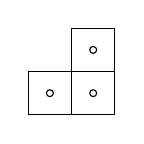
\begin{tikzpicture}[scale=0.55]
 \draw (0,0) rectangle (1,1);
 \draw (1,0) rectangle (2,1);
 \draw (1,1) rectangle (2,2);
 \draw (0.5,0.5) circle (0.08);
 \draw (1.5,0.5) circle (0.08);
 \draw (1.5,1.5) circle (0.08);
\end{tikzpicture}}}
$\Gamma(\theta)$ — длина границы.
$U(\theta)$ — число соседей (пар соседей).
Распред. Гиббса
\begin{gather*}
 p(\theta)=
 \frac{\exp\{U(\theta)/T\}}
 {\displaystyle\sum_{\theta\in\mathcal{B}(V_\ell,N)}\exp\{U(\theta)/T\}}
 =\frac{\exp\{-\Gamma(\theta)/(2T)\}}
 {\displaystyle\sum_\theta\exp\{-\Gamma(\theta)/(2T)\}}.
\end{gather*}
[Под первой суммой:] все распол.
\begin{gather*}
 (\text{т. к. }2U(\theta)=2\nu N-\Gamma(\theta)).
\end{gather*}
\underline{Фазовый переход.}
Пусть решётка растёт $\ell\to\infty$,
и пусть $N_\ell\to\infty$.
Предел $V_\ell/N_\ell\to v$ — уд. объём.
Оказ., что
\begin{gather*}
 \frac1N\log\sum_\theta\exp\{U(\theta)/T\}\longrightarrow f(v,T).
\end{gather*}
\Unclear{GELFAND-P000008}{name-van-hove}{Под пределом имя читается «Ван Хов» или «Ванхов»; середина и конец густо переписаны.}
$(v,T)$ наз. точкой фаз. перехода, если
\begin{gather*}
 \frac{\partial f(v,T)}{\partial v}=0
 \quad\text{в нек. окр. при }T=\mathrm{const}.
\end{gather*}
\Unclear{GELFAND-P000008}{temperature-relation}{Между $T$ и const знак похож на $=$ или $\ne$; кандидат $=$ сохранён, чтение не утверждается.}
\Incomplete{GELFAND-P000008}{margin-left}{На самом левом краю виден узкий обрезанный столбик рукописных окончаний соседнего текста; непрерывные слова восстановить нельзя.}



\SourcePage{GELFAND-P000009}{5}
(Т. к. ф-я линейна, a priori она выпукла.)
\begin{gather*}
 Q(T)=\frac{S_\nu e(1-e^{-1/(2T)})}
 {3(1+e^{-\nu/T})}
 \sum_{k=2\nu}^{\infty}3\exp\{-1/(2T)\}^{k}
 k^{\frac\nu{\nu-1}}.
\end{gather*}
[После первого равенства зачёркнутый фрагмент:]
\Unclear{GELFAND-P000009}{q-formula}{Зачёркнутый знак после $=$ не читается. В числителе множитель после $S_\nu$ похож на $e$; верхний предел суммы похож на $\infty$ или двойной штрих. Степень $k$ может относиться также к множителю $3$, но на скане видна у закрывающей фигурной скобки. Варианты не заменены стандартной формулой.}
$S_\nu$ — объём $\nu$-мерн. сф. с $1$ пов.
\begin{gather*}
 S_2=\frac1{4\pi},\qquad S_3=\frac1{C\sqrt\pi}.
\end{gather*}
\Unclear{GELFAND-P000009}{sphere-constant}{Первый множитель знаменателя $S_3$ похож на $C$, $c$ или $6$; запись $C$ — только кандидат.}
Если
\begin{gather*}
 Q(T)<\frac1v<1-Q(T),
\end{gather*}
то имеет место фазовый переход.
\SourceFigure{GELFAND-P000009}{diagram-coexistence-dome}{Оригинал и прежнее наборное воспроизведение.\par\smallskip\centering\resizebox{.93\linewidth}{!}{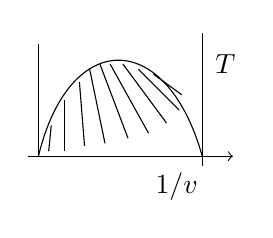
\begin{tikzpicture}[scale=0.65]
 \draw (-0.2,0)--(3.2,0);
 \draw[->] (3.2,0)--(3.8,0);
 \draw (0,0)--(0,2.2);
 \draw (3.2,-0.2)--(3.2,2.4);
 \draw (0,0).. controls (0.6,2.5) and (2.5,2.5)..(3.2,0);
 \draw (0.2,0.1)--(0.25,0.6);
 \draw (0.5,0.1)--(0.5,1.1);
 \draw (0.9,0.2)--(0.8,1.45);
 \draw (1.3,0.25)--(1,1.7);
 \draw (1.75,0.35)--(1.2,1.8);
 \draw (2.15,0.45)--(1.4,1.8);
 \draw (2.5,0.65)--(1.65,1.8);
 \draw (2.75,0.9)--(1.95,1.7);
 \draw (2.8,1.2)--(2.25,1.6);
 \node at (3.65,1.8) {$T$};
 \node at (2.7,-0.6) {$1/v$};
\end{tikzpicture}}}
[Разделительная черта.]

$S$ — подкуб. $S_\ell\subset V_\ell$.
$K_\ell$ — сторона $S_\ell$.
\begin{gather*}
 0<d<\frac{K_\ell}{\ell}<1-d.
\end{gather*}
Ввод. случ. велич.
$\mu(S_\ell)$ — число точек расп. $\theta$, попавших в $S_\ell$.
$\mu_{S_\ell}(\theta)$.
Если
\begin{gather*}
 \mathsf{P}\left\{
 \left|\frac{\mu_{S_\ell}(\theta)}{K_\ell^\nu}-\frac1v\right|
 \right\}>\varepsilon\}\overset{/}{\longrightarrow}0,
 \qquad\varepsilon>0,
\end{gather*}
то есть фаз. переход.
\Unclear{GELFAND-P000009}{probability-brace}{На скане после правой черты видна фигурная скобка перед $>\varepsilon$ и ещё одна после $\varepsilon$. Эта несогласованная запись сохранена; кандидат обычного события — модуль больше $\varepsilon$ внутри одной пары скобок.}
[Под первой дробью:] плотн. в подкубе.
[Под $1/v$:] плотн. во всём кубе.
И близкое условие необходимо.
(Физ. смысл — сосущ. $2$-х фаз.)

\SourceFigure{GELFAND-P000009}{diagram-corner-cluster}{Оригинал и прежнее наборное воспроизведение.\par\smallskip\centering\resizebox{.93\linewidth}{!}{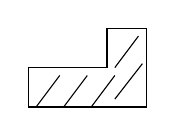
\begin{tikzpicture}[scale=0.5]
 \draw (0,0)--(3,0)--(3,2)--(2,2)--(2,1)--(0,1)--cycle;
 \draw (0.2,0)--(0.8,0.8);
 \draw (0.9,0)--(1.5,0.8);
 \draw (1.6,0)--(2.2,0.8);
 \draw (2.2,0.2)--(2.9,1.1);
 \draw (2.2,1)--(2.8,1.8);
\end{tikzpicture}}}
Граница в расп. на компоненты —
— но связь через уголки ($\nu=2$) и ребро ($\nu=3$)
не учитывается.
\begin{gather*}
 \Gamma(\theta)=\sum_i\Gamma_i(\theta).
\end{gather*}
$\Gamma_i(\theta)$ — дл. или площ. компон. границы.
\underline{Определение.} Выделим спец. расположение.
Зав. от $3$-х чисел $N<\infty$, $D<\infty$, $\delta>0$.
\Unclear{GELFAND-P000009}{finite-parameter}{Первая буква похожа на $N$, но допускает $M$; увеличенный фрагмент не снимает различия. Она не согласована автоматически с верхним пределом суммы следующего кадра.}
Циклы занумер. по убыв. длин
\begin{gather*}
 \Gamma_1(\theta)\ge\Gamma_2(\theta)\ge\cdots .
\end{gather*}



\SourcePage{GELFAND-P000010}{unlabelled}
Усл.
\begin{gather*}
 1)\quad\sum_{i=1}^{M}\Gamma_i(\theta)\le D\ell^{\nu-1}.
\end{gather*}
(Порядок пов. большого куба.)
\begin{gather*}
 2)\quad\sum_{i=M+1}^{\infty}
 \bigl(\Gamma_i(\theta)\bigr)^{\frac\nu{\nu-1}}
 \le\frac{\min(N_\ell,V_\ell-N_\ell)}{S_\nu}(1-\delta).
\end{gather*}
\Unclear{GELFAND-P000010}{small-cycles-sign}{Знак неравенства перед дробью густо переписан; кандидаты $\le$ и $<$. Первый параметр верхнего предела первой суммы похож на $M$ или $N$.}
\begin{gather*}
 S_\nu\bigl(\Gamma_i(\theta)\bigr)^{\frac\nu{\nu-1}}
\end{gather*}
Площ. круга с длиной $\Gamma_i$.
Max объём имеет шар, это оц. сверху для объ. об. внутри циклов.
(Он $<$ чем нужно, чтобы помест. все занятые точки.)
([Слово зачёркнуто; сверху вставлено:] объём.
Внутри мелких циклов $<$ заштрих. площ.
и белая площадь.)
\Unclear{GELFAND-P000010}{small-volume-cancellation}{Слово под вставленным «объём» густо зачёркнуто и не читается. «Площ.» в двух строках оставлено как на скане, без замены на объём.}

\SourceFigure{GELFAND-P000010}{diagram-nested-cycles}{Четыре вложенные округлые границы: внешнее заштрихованное кольцо, белый промежуток и внутреннее кольцо с белой серединой. Неровности и слияния отдельных штрихов показаны на оригинале.\par\smallskip\centering\resizebox{.93\linewidth}{!}{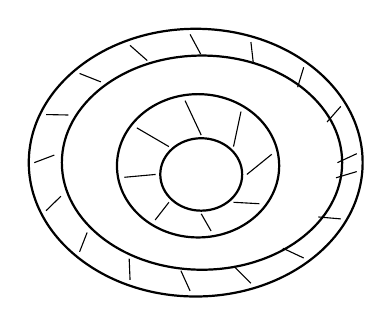
\begin{tikzpicture}[x=1cm,y=1cm]
\draw[thick](0,0)ellipse(2.12 and 1.7);\draw[thick](.08,0)ellipse(1.78 and 1.36);
\draw[thick](.03,-.04)ellipse(1.03 and .91);\draw[thick](.07,-.15)ellipse(.52 and .46);
\foreach \a in{0,22,...,352}{\draw({1.8*cos(\a)},{1.38*sin(\a)})--({2.05*cos(\a+4)},{1.63*sin(\a+4)});}
\foreach \a in{0,45,...,315}{\draw({.58*cos(\a)+.07},{.5*sin(\a)-.15})--({.95*cos(\a+10)+.03},{.84*sin(\a+10)-.04});}
\end{tikzpicture}}\par{\scriptsize Четыре границы, два заштрихованных кольца; схема без масштаба.}\par}
Нельзя загнать туда ни все точки, ни все пустые места.
Пример расп., когда не вып.
\SourceFigure{GELFAND-P000010}{diagram-phase-mixture}{Прямоугольник разделён почти горизонтальной кривой: сверху три маленькие округлые области, снизу штриховка и несколько округлых незаштрихованных областей. Точные границы и число нижних областей не уверены.\par\smallskip\centering\resizebox{.93\linewidth}{!}{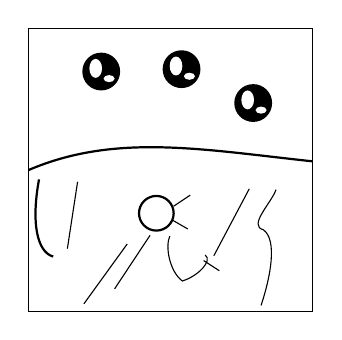
\begin{tikzpicture}[x=1cm,y=1cm]
\draw(0,0)rectangle(3.6,3.6);
\draw[thick](0,1.8)..controls(1.1,2.27)and(2.2,2.06)..(3.6,1.91);
\foreach \x/\y in{.92/3.05,1.94/3.08,2.85/2.65}{\fill(\x,\y)circle(.24);\fill[white](\x-.07,\y+.04)ellipse(.08 and .12);\fill[white](\x+.1,\y-.09)ellipse(.07 and .045);}
\draw[thick](1.62,1.25)circle(.22);
\draw(1.84,1.34)--(2.05,1.48);\draw(1.83,1.16)--(2.02,1.05);
\draw(1.79,.96)..controls(1.73,.82)and(1.79,.51)..(1.95,.39)..controls(2.15,.45)and(2.34,.65)..(2.24,.72);
\draw(2.22,.65)--(2.42,.52);
\draw[thick](.13,1.68)..controls(.03,1.14)and(.1,.76)..(.31,.7);
\draw(.62,1.65)--(.49,.8);\draw(.7,.1)--(1.25,.86);\draw(1.09,.29)--(1.54,.97);\draw(2.35,.71)--(2.8,1.56);\draw(2.95,.08)..controls(3.07,.44)and(3.16,.91)..(2.98,1.04)..controls(2.78,1.09)and(3.08,1.38)..(3.14,1.55);
\end{tikzpicture}}\par{\scriptsize Частичная схема: неясный нижний контур не замкнут.}\par}
Это фаз. переход.
Все св. к $2$-м леммам.

$1)$ $\exists M,D,\delta$, что
вер. вып. условий $\longrightarrow1$,
если вып. сформ. условие.
[Под параметрами:] ни от кого не зависят.
\Unclear{GELFAND-P000010}{theorem-condition}{В строке после «если вып.» слово выглядит «сформ.» или «строгое»; не дополнено по смыслу.}

$2)$ \underline{Лемма $2$.}
Если почти все расп. особые, то фаз. переход.
\underline{Идея док. леммы $2$.}
$G$ — объ., об. внутри мал. циклов.
\begin{gather*}
 G\le N_\ell(1-\delta),\qquad
 \frac{G}{V_\ell}\le\frac1v(1-\delta).
\end{gather*}
\SourceFigure{GELFAND-P000010}{diagram-grid}{Прямоугольная решётка пять на пять; выделена вторая клетка слева в четвёртом ряду сверху. Подпись: «Разбили на подкубы».\par\smallskip\centering\resizebox{.93\linewidth}{!}{\begin{tikzpicture}[x=.64cm,y=.64cm]
\draw[step=1](0,0)grid(5,5);\draw[line width=2.2pt](1,1)rectangle(2,2);
\node[anchor=west,align=left,font=\small]at(5.2,3){\GridWords};
\end{tikzpicture}}\par{\scriptsize Сетка 5×5; выделена клетка (2,4), считая слева и сверху.}\par}
Сущ. подкуб $S_\ell$:
\begin{gather*}
 \frac{G\cap S_\ell}{V_\ell}\le\frac1v(1-\delta).
\end{gather*}
\Unclear{GELFAND-P000010}{last-fraction}{В числителе перед $\cap S_\ell$ густой знак похож на $G$, в знаменателе явно похоже на $V_\ell$. Сохранён кандидат; мера пересечения и объём подкуба не подставлены по смыслу.}


\Needspace{5\baselineskip}
\SourcePage{GELFAND-P000011}{6}
Пусть все большие циклы \Unclear{GELFAND-P000011}{top-line}{со / $\infty$ окружают. [двухпетлевой знак перед глаголом неуверен]}.

2 случая.
\SourceFigure{GELFAND-P000011}{diagram-01}{Два маленьких прямоугольника: в левом четыре закрашенных кружка; в правом четыре круглых знака, три с видимым светлым центром, нижний правый темнее и плотнее обведён. Внутри правого прямоугольника дополнительные мелкие, местами дугообразные штрихи. Их значение и точные направления не установлены.\par\smallskip\centering\resizebox{.93\linewidth}{!}{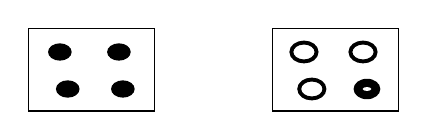
\begin{tikzpicture}[x=1cm,y=1cm,line width=.5pt]
\draw(0,0)rectangle(1.6,1.05);\draw(3.1,0)rectangle(4.7,1.05);
\foreach \x/\y in{.4/.75,1.15/.75,.5/.28,1.2/.28}{\fill(\x,\y)ellipse[x radius=.15,y radius=.11];}
\foreach \x/\y in{3.5/.75,4.25/.75,3.6/.28}{\draw[line width=1.4pt](\x,\y)ellipse[x radius=.16,y radius=.12];}
\fill(4.3,.28)ellipse[x radius=.17,y radius=.13];\fill[white](4.3,.28)ellipse[x radius=.055,y radius=.025];
\end{tikzpicture}}\par{\footnotesize Частичная схема: мелкие внутренние штрихи остаются на оригинале.}}

\underline{Лемма.} \Unclear{GELFAND-P000011}{upper-middle}{Непрс. [неуверенное сокращение]} границу из $k$ [зачёркнуто: \Unclear{GELFAND-P000011}{upper-right-cancellation}{точк. [чтение зачёркнутого неуверенно]}; сверху/ниже вписано: звеньев] $\leq 3^k$.

Выигрыш $3$, проиг.
\SourceFigure{GELFAND-P000011}{diagram-02}{Под словами о выигрыше и проигрыше нарисованы горизонтальная линия с короткими крайними штрихами и вертикальный отрезок вниз; это исходная схема без уверенно прочитанных подписей.\par\smallskip\centering\resizebox{.93\linewidth}{!}{\begin{tikzpicture}[x=1cm,y=1cm,line width=.6pt]
\draw(-1.2,0)--(.5,0);\draw(.78,0)--(1.2,0);\draw(0,.12)--(0,-.9);
\end{tikzpicture}}\par{\footnotesize Видимые штрихи без приписанных подписей и стрелок.}}
\begin{equation*}
\exp\left\{-\frac{1}{2T}\right\},\qquad
\left(3\exp\left\{-\frac{1}{2T}\right\}\right)^k.
\end{equation*}

\underline{Зад.} (нереш.)
Пусть $N$ велико. Повор. с вер. $\frac13$, но запрещ. [зачёркнуто: \Unclear{GELFAND-P000011}{middle-cancellation-01}{не [неуверенный кандидат короткого слова]}] возвращ.
Каково [зачёркнуто: \Unclear{GELFAND-P000011}{middle-cancellation-02}{вер. ... [первое сокращение-кандидат; следующая отменённая запись не читается]}] мат. ожид. расстояния, на к-рое он уйдёт за $N$ шагов.

(Если разреш. возвращ., то $\sim\sqrt n$.)
Если разреш. возвр., то
\Unclear{GELFAND-P000011}{middle-bound}{$(\geq2{,}6^n\ \text{но}\ <2{,}8^n,\ \text{гипотеза}\ e^n)$; первый знак также может читаться $>$; дополнительные штрихи неуверенны}.

[Горизонтальный разделитель.]

$28/\mathrm{IX}$ \underline{Сигал.}
Теория ф-й на мн. реш. релятив. дифф. ур-я.
[На левом поле: Все они запис. так.]
\begin{equation*}
u'=Au+K(u)\qquad(A)\qquad u(t),\quad -\infty<t<+\infty,
\end{equation*}
\begin{equation*}
A=-A^*,\qquad u\in L^2,\qquad u(t)\in H.
\end{equation*}
$K$ --- зад. нелин. оператор.
В $\int$ форме
\begin{equation*}
u(t)=e^{A(t-t_0)}u(t_0)+\int_{t_0}^{t}e^{A(t-s)}K(u(s))\,ds\qquad(B).
\end{equation*}
Когда $K\in C^1$, т. е. $\partial_uK=K_u$ сущ. по Фреше и непр., то каждое реш. (B) есть реш. A (если $u(t)$ из обл. опр. A).

[Горизонтальный разделитель.]

Пусть (B) им. реш. в целом $\forall$ нач. данным в $t_0$ ($u_0$).
(И $K\in C^1$.)
В квант. мех.
\begin{equation*}
\square\varphi=f(\varphi)
\end{equation*}
[Под знаком $\square$: даламбертиан.]
\begin{equation*}
u(t)=[\varphi(\cdot,t),\dot\varphi(\cdot,t)],\qquad
\varphi=\varphi(\vec x,t).
\end{equation*}
$K$ --- нелин. опер. \Unclear{GELFAND-P000011}{bottom-line}{Немыц. / Намыц. [последнее сокращение неуверенно]}.



\Needspace{5\baselineskip}
\SourcePage{GELFAND-P000012}{unlabelled}
\begin{equation*}
\|[\varphi,\omega]\|\qquad
\square\varphi=m^2\varphi+f(\varphi)
\end{equation*}
[Под формулой: Более кр. форма.]
\begin{equation*}
B=\sqrt{m^2I-\Delta},\qquad
\|[\varphi,\omega]\|=\|B\varphi\|_{L^2}^{2}+\|\omega\|_{L^2}^{2}.
\end{equation*}
\Unclear{GELFAND-P000012}{upper-norm}{В левой части последней формулы над нормой квадрат не виден; правая часть содержит квадраты. Запись сохранена без математического исправления.}
$A$ зад. матрицей 2-го порядка
\begin{equation*}
\begin{pmatrix}0&I\\-B^2&0\end{pmatrix}.
\end{equation*}
Он не самосопр., но в этой норме самосопр.
\Unclear{GELFAND-P000012}{upper-selfadjoint}{Слово «самосопр.» прочитано так в обоих местах; возможное сокращение и согласование с предыдущей записью $A=-A^*$ требуют сверки.}
Любое ур-е релятив. физ. запиш. так.

$M$ --- совок. всех решений.
\begin{equation*}
M=[u(\cdot);\ (**)\ \text{удовл.}]
\end{equation*}
[Справа/под формулой: от $t$; \Unclear{GELFAND-P000012}{upper-right-note}{различные B. [неуверенное чтение подчёркнутой пометы]}]
Пусть теперь $K\in C^\infty$.
$M$ --- Банахово многообр. (у люб. точки есть окр., гомеом. бан. [зачёркнуто: \Unclear{GELFAND-P000012}{middle-cancellation}{неразборчивое слово}] пр-ву, переход --- $C^\infty$ (по Фреше) ф-и).
\begin{equation*}
S_t:M\longrightarrow H,\qquad u(\cdot)\longmapsto u(t).
\end{equation*}
[Справа: оператор. \Unclear{GELFAND-P000012}{middle-right-note}{$\text{мн. реш.}\longrightarrow H$ / $\text{им. реш.}\longrightarrow H$ [первое сокращение неуверенно; конечная стрелка и $H$ видны]}]
\underline{Теорема.} Сущ. единственная $C^\infty$-многообразная структура, что отобр. $S_t$ --- $C^\infty$-изоморфизм.
$u(t,u_0)$ зависит от $u_0$ $C^\infty$-обр.

Истин. многообр.
Есть кас. пр-во $T_{u(\cdot)}$.
Кас. отобр.
\begin{equation*}
dS_t:T_{u(\cdot)}\longrightarrow T_{u(t)}.
\end{equation*}
Кон. $\forall$ точки изом. самому пр-ву.
\begin{equation*}
\lambda\in T_{u(\cdot)},\qquad dS_t(\lambda)=v(t)\in H.
\end{equation*}
Получ. --- каждому кас. вектору соотв. ф-я.
[Подчёркнуто и зачёркнуто: Лемма.]
Обозн. $v(t)$ (не знач. $v$ в т. $t$), ур. вар. ур-е 1-го пор.
\begin{equation*}
v'=Av+K_{u(\cdot)}.
\end{equation*}
\Unclear{GELFAND-P000012}{lower-variation}{После $K_{u(\cdot)}$ отдельный множитель $v$ на этой строке не виден; запись оставлена как в источнике.}
Реш. этого ур-я происх. из кас. вект. $\lambda$ и наоборот.

1) Канонич. дифф. форма на $M$.

2) Скобки Пуассона (анал. с конечномерн. случаем).



\Needspace{5\baselineskip}
\SourcePage{GELFAND-P000013}{7}
3) Вект. поля в $M$. В их терм. будут \Unclear{GELFAND-P000013}{top-line}{зд. [последнее сокращение неуверенно]}.

4) Канонич. коммут. соотн.

5) Будет дано предст. и явное опр. опер.

$5/\mathrm X$. \underline{Сигал.}
I. Ренормализ. ур-е поля.
1) Вывод. 2) Сущ. и ед.

II. Опред. матрицы рассеяния $S$.
A. Классич. $S$-оп.
B. Распр. обобщ. вер. распред. в нелин. сл.

III. Обсужд. вопр. интерпр. с теор. частиц.

[Горизонтальный разделитель.]

Рассм. ур-е
\begin{equation*}
\square\widetilde\varphi=m^2\widetilde\varphi+\widetilde\varphi^3,
\end{equation*}
\begin{equation*}
[\widetilde\varphi(\vec x,t),\widetilde\varphi(\vec x',t)]
=0=[\dot{\widetilde\varphi}(\vec x,t),\dot{\widetilde\varphi}(\vec x',t)].
\end{equation*}
\Unclear{GELFAND-P000013}{middle-commutator}{Кандидаты исходной строки: $[\widetilde\varphi(x),\widetilde\varphi(x')]=i\delta'(x-x')$ / $[\widetilde\varphi(x),\dot{\widetilde\varphi}(x')]=i\delta(x-x')$. Точка над второй буквой, вид дополнительного штриха после $\delta$ и точное положение аргументов не вполне различимы.}

\underline{Loran Schwartz.}
Есть 2 типа мер: меры Радона и просто меры [над последним словом вставлено: абстр.].
Пока огранич. $+$ меры.
\underline{Абстр. мера} на мн-ве $X$, $F$ --- $\sigma$-алгебра.
$\mu$ --- мера. $\mu$ --- $\sigma$-адд. по $F$.

[Горизонтальная линия.]

Когда уже зад. мера, то можно рассм. на $\mu$-изм. мн-ва, $F_\mu$ на $X$ и интегр. измеримые ф-и.
\begin{equation*}
f:X\longrightarrow F,\qquad \int_Xf(x)\,d\mu(x).
\end{equation*}
[Справа: знач. в бан. пр-ве; $F$ --- Бан. пр-во.]

[Горизонтальная линия.]

\underline{Радон. мера.} $X$ --- произвол. лок. компактное.
$C(X)$ --- непр. ф-и с комп. носителями с топ. инд. предела,
и пусть $C'(X)$ сопр. пр-во.
Его элем. --- мера на $X$.



\Needspace{5\baselineskip}
\SourcePage{GELFAND-P000014}{unlabelled}
$\mu$ --- полож., если $\mu(\varphi)\geq0$ при $\varphi\geq0$.
Мера ограничена, если
\begin{equation*}
|\mu(\varphi)|\leq C\max|\varphi|.
\end{equation*}
2-е опрд. --- огранич. полож. Рад. мера.
С ней делается тоже Леб. расширение.
И $\int$ тоже сущ. (знач. в бан. пр-ве).

$\sigma$-поле, постр. по Рад. мере, зависит от $\mu$, но сущ. не завис. от $\mu$ (существ.) --- поле борел. мн-в
(\Unclear{GELFAND-P000014}{upper-borel-note}{min сод. замкн. и откр. [начало скобочной пометы неуверенно]}).

[Горизонтальный разделитель.]

Причина предпочтения радоновых мер различным мат.?
Радон. меры сущ. только на лок.-комп. пр-вах (огранич. теор. вер.).
Но [зачёркнуто: \Unclear{GELFAND-P000014}{middle-cancellation-01}{два коротких неразборчивых слова}] Рад. меры удобнее.
\Unclear{GELFAND-P000014}{middle-uniqueness}{Для правых мер есть разлож. / различ. единицы (если [зачёркнутое начало] мера $=0$ на сист. окр., то она вообще ноль). [Первое определение мер и сокращение перед «единицы» неуверенны.]}
Есть 5--15 теор., верных для Рад. мер (только).

\begin{equation*}
X\overset f\longrightarrow Y
\end{equation*}
[Под стрелкой: топ. пр-ва.]
[Зачёркнуто: \Unclear{GELFAND-P000014}{middle-cancellation-02}{короткое слово перед «Выделим»}.]
Выделим на $X$ и на $Y$ Борелевское поле и абстр. меру $\mu$ на $X$.
И пусть $A\subset Y$.
Тогда есть мера $f(\mu)$ в $Y$:
\begin{equation*}
f(\mu)(B)=\mu(f^{-1}(B)).
\end{equation*}
Но если $B$ --- произв. подмн. $A\subset X$, то [зачёркнут одиночный знак]
\begin{equation*}
f(\mu)(A)\qquad \mu(f^{-1}(A)).
\end{equation*}
\Unclear{GELFAND-P000014}{lower-set-names}{В исходной записи чередуются $A$ и $B$ и перед второй парой формул читается $A\subset X$; буквенные обозначения не согласованы редактором.}
Можно пок., что если левая часть им. смысл, то правая тоже и они равны, но обратное неверно.
[Зачёркнуто: \Unclear{GELFAND-P000014}{lower-cancellation}{неразборчивое начало строки}.]
\begin{equation*}
A\ \text{---}\ f(\mu)\text{-изм.}\ \Longrightarrow\ f^{-1}(A)\ \mu\text{-изм.}
\end{equation*}
Если $\mu$ --- мера Радона, то эквивалентность.

\underline{Пример (противореч.)}
\begin{equation*}
X\subseteq Y=[0,1]
\end{equation*}
так, что $X$ --- неизмеримое по Лебегу мн-во,
$Y\setminus X$ имеет внутр. меру $0$ (или внешн. мера $X=1$).
Подмн. $X$ --- борелево $\Longleftrightarrow$ оно пересеч. с бор. мн. $Y$.
$\mu$ --- абстр. мера.



\Needspace{5\baselineskip}
\SourcePage{GELFAND-P000015}{8}
\underline{Опрд.} $\mu(D)$.
$D\subset X$ --- борел.
\begin{equation*}
D=X\cap E,\qquad E\ \text{--- бор. в }Y,
\end{equation*}
\begin{equation*}
\mu(D)\underset{\mathrm{def}}=dx(E)
\end{equation*}
[Под $dx(E)$: леб. мера.]
\Unclear{GELFAND-P000015}{upper-lebesgue-notation}{В записи $dx(E)$ обе буквы стоят на основной строке; регистр второй буквы не вполне различим: $dx(E)$ / $dX(E)$. Подстрочный индекс не добавлен.}
Мера одна и та же (\Unclear{GELFAND-P000015}{upper-null-note}{отлич. на мн-во вн. меры 0 [скобочная помета неуверенно]}).
Мы опр. абстр. меру на $X$. Образ её
[Следующая строка повторяет: образ её] $dx$.
Возьмём какое-нибудь (не бор.) подмн. $Y\setminus X$.
Оно неизмер., но его прообраз пуст и значит измерим.

Цель докл. --- пок., что не нужна лок.-комп.
Пусть $\mu$ --- мера на $F_B$, тогда $\mu$ есть Рад. мера, если она внутр. комп. рег.
\begin{equation*}
\mu\ \text{Радонова}\ \Longleftrightarrow
\forall B,\ \forall\varepsilon>0\ \exists\text{ комп. }\subset B,\qquad
\mu(b-k)\leq\varepsilon.
\end{equation*}
\Unclear{GELFAND-P000015}{upper-regularity}{В разности читаются строчные $b-k$, хотя перед ней написано $\forall B$. Между «комп.» и $\subset B$ отдельная буква множества не видна; она не подставлена по смыслу.}
[Горизонтальный разделитель.]

\underline{$X$ --- топ. пр-во.}
Найдём меру, обл. всеми св-ми Рад. лок.-комп. мер.
Пусть она опр. (завед.) на бор. мн-вах.
\underline{Опрд. рад. меры, год. не только для лок. комп.}
Пусть $X$ --- вп. регулярно (они могут быть вложены в комп. пр-ва max идеалов).
\begin{equation*}
X,\qquad \widehat X\ \text{--- чех. пополнение }X
\end{equation*}
(max ид. алг. непр. ф-й).
\begin{equation*}
X\overset i\longrightarrow\widehat X.
\end{equation*}
Полная рег. озн., что это гомеом. отобр., а не только инъект. отобр.
Другое опрд. рад. меры над $X$ --- радон. мера на $\widehat X$, при к-рой
\begin{equation*}
\mu(\widehat X\setminus X)=0.
\end{equation*}
Можно пок. эквивалентность.
\underline{В лок. комп.}
\begin{equation*}
\mu\ \mathrm{Rad}\ \Longleftrightarrow\ \forall B\text{ комп.}\ \forall\varepsilon>0\ \exists\text{ комп.}\quad
\mu(B-k)<\varepsilon.
\end{equation*}
\Unclear{GELFAND-P000015}{lower-regularity}{В разности второй знак похож на строчное $k$; первый читается как $B$, но регистр не вполне уверен ($B-k$ / $b-k$). После «комп.» отдельная буква множества и условие включения не видны. Не дополнено по предыдущей формуле.}
Все св-ва Рад. мер выполняются.
Док-во теор. верно в $\widehat X$ и ост. почти трив.
Есть единств. искл. --- [зачёркнуто: \Unclear{GELFAND-P000015}{bottom-cancellation}{св-ва ... бор. ... [видимые фрагменты-кандидаты под горизонтальной чертой; полная отменённая фраза не читается]}] пр-в.
--- нельзя опр. носит. произв. рад. мер.



\Needspace{5\baselineskip}
\SourcePage{GELFAND-P000016}{unlabelled}
$X\subset K_0$ в комп. пр-во (любое). Тогда сущ. аналогичное опр. Рад. мер.
Мы получим тот же закон.

[Горизонтальный разделитель.]

Сравним с опр. ядерного пр-ва (пр-ва в к-рых 2 опр. тенз. произв. совп.).
\begin{equation*}
a(X)\supset R(X).
\end{equation*}
\Unclear{GELFAND-P000016}{upper-space-symbol}{Первый символ в включении похож на строчное $a$ с крупной петлёй; возможное $A$ или каллиграфическая форма не вполне исключены.}
Радон. пр-во, если $\forall$ абстр. мера на нём --- радонова.

3 св-ва рад. пр-в.
1) Если $X$ рад. и $Y\subset X$, то $Y$ радоново $\Longleftrightarrow$ оно универс. измеримо в $X$
(изм. по отн. ко всем рад. мерам --- напр. Борелевское, суслинское и аналитич.).

Важн. критерий.
2) Если $X$ --- рад., то оно универс. измеримо, т. е. изм. $\forall$ объемл. пр-ву и $\forall$ мере.
\Unclear{GELFAND-P000016}{middle-universal}{Сокращение после «изм. \(\forall\)» читается как «объемл.» / «объем.»; окончание и наличие надстрочного знака не вполне различимы. Не раскрыто до полного слова.}
Теор. вер. --- всегда опр. вер.

3) Пример широк. класса рад.-пр-в.
Распределения, непр. ф-и и т. д.?
Пусть $E$ --- Т. Л. К. --- сепарабельное пр-во Фреше или их счётный инд. предел.
$F$ --- такое же.
Тогда $\operatorname{Hom}(E,F)$ такие же (снабж. любой топ. между поточ. и комп. сход.).
В частности, двойств. пр-во, само пр-во ($R\longrightarrow E$).
Все пр-ва обобщ., $C^\infty$ ф-й.
И опер. $\mathcal L(S,S)$ тоже радоново пр-во.
\Unclear{GELFAND-P000016}{lower-operator-space}{Над/рядом с закрывающей скобкой имеется короткая помета «ф-и». Отдельный штрих после $\mathcal L(S,S)$ не отделяется уверенно от пометы и скобки; кандидат $\mathcal L(S,S)'$ остаётся неуверенным.}

\underline{Прилож.} Рассм. стох. процесс, зад. как вер. на пр-ве всех ф-й с простой сходим. (поточ.) (мера в этом пр-ве).
Возьмём подпр-во непр. ф-й. Оно измер. в $R^R$.



\Needspace{5\baselineskip}
\SourcePage{GELFAND-P000017}{9}
И значит, вероятность ф-и быть непр. всегда сущ.
Пусть она равна $1$. Тогда есть вер. распр. на этом подпр. и она может быть опр. как просто рад. мера на $C$.
Она соср. на сч. числе комп. мн-в (равностеп. непр.).
Если вер. ф-и быть непр. $1$, то с вер. $1$ все эти ф-и им. общ. модуль непр.
Это верно $\forall$ стох. процесса ($\exists$ общ. mod непр. с вер. $1$).

[Большая незаписанная область; на границе в середине кадра видны отдельные небольшие горизонтальные/дугообразные штрихи.]
\Unclear{GELFAND-P000017}{middle-boundary-strokes}{На горизонтальной границе большой незаписанной области сохранились только нижние части отдельных буквоподобных штрихов; целое слово не читается.}

$12/\mathrm X$.
\underline{Гиндикин.}
\underline{Вейль.} $G$ --- полупр. гр. Ли, что среди вещ. комп. нет матр. 2-го пор.
\Unclear{GELFAND-P000017}{middle-group-hypothesis}{Сокращения «вещ. комп.» и «матр. 2-го пор.» оставлены по видимой строке, без подстановки теоретической формулировки.}
$\Gamma$ --- дискр. подгруппа, $G/\Gamma$ компактно.
Рассм. деформации $\Gamma$: $\gamma(t)$, $\forall t$ дискр. гр. $\Gamma^{(t)}$.
Трив. способ при пом. внутр. автом.
\begin{equation*}
g(t)\gamma g(t)^{-1}.
\end{equation*}
Факторгр. одна и та же.
При этих усл. всякие деформ. тривиальны.
Дост. док., что
\begin{equation*}
H^1(\Gamma,\mathfrak g)=0.
\end{equation*}
$\mathfrak g$ --- алгебра Ли, на ней предст. $\Gamma$.
Если $\Gamma$ не дискр., то теор. Вейля имеет место, хотя $H^1(\Gamma,\mathfrak g)\ne0$.
\Unclear{GELFAND-P000017}{lower-nondiscrete}{В условии читается «не дискр.»; возможная исходная неточность или сокращение не исправлены.}
Есть представл. $\rho(\gamma)$ в $V^d$. Тогда разм.
\begin{equation*}
p=(2g-2)d+i+i'.
\end{equation*}



\Needspace{5\baselineskip}
\SourcePage{GELFAND-P000018}{unlabelled}
\underline{Лоран Шварц.}
\begin{equation*}
E\ \text{---}\ \mathrm{TVS\ LCH\ QC}.
\end{equation*}
[От $H$ в сокращении проведена помета: хаусдорфова.]
Лок. вып. топ. вект. пр-во, почти полное (всякое замкн. огр. мн-во полное).
$\mathcal H$ --- гильб. подпр-во $E$.
\begin{equation*}
\mathcal H\subset E.
\end{equation*}
[Под включением: отобр. непр.; справа: в $\mathcal H$ гильб. метрика.]
Гильб. топология не совпа., а сильнее топ. в $E$.
\underline{Пример.}
\Unclear{GELFAND-P000018}{upper-example}{Запись включения: $L^2\subset\mathcal D^1$ / $L^2\subset\mathcal D'$; толстый знак справа над $\mathcal D$ похож и на $1$, и на штрих.}
Ещё прим. --- пр-во констант:
\begin{equation*}
(\alpha\mid\beta)=\alpha\overline\beta.
\end{equation*}
\begin{equation*}
\mathcal H\in\mathrm{Hilb}(E)\ \text{--- все гильб. подпр-ва}.
\end{equation*}
[На левом поле повторено: $\mathrm{Hilb}(E)$, со стрелкой к следующему заголовку.]
Абстрактная конич. структура.
Надо определить слож., умн. на $+$ числа и упорядочить.
\begin{equation*}
\mathcal H\in\mathrm{Hilb}(E),\quad \lambda\geq0,\quad \lambda\mathcal H,\quad
\mathcal H_1+\mathcal H_2,\qquad \mathcal H_1\leq\mathcal H_2.
\end{equation*}
При $\lambda=0$, $\lambda\mathcal H$ --- 0-е подпр-во.
При $\lambda\ne0$, $\lambda\mathcal H$ есть то же пр-во со скал. произв.
\begin{equation*}
(h\mid k)_{\lambda\mathcal H}=\frac1\lambda(h\mid k)_{\mathcal H}.
\end{equation*}
$\mathcal H_1+\mathcal H_2$.
Если 0-е пересеч., то прямое.
\begin{equation*}
\|h\|_{\mathcal H_1,\mathcal H_2}
=\inf\left(\|h_1\|_{\mathcal H_1}^2+\|h_2\|_{\mathcal H_2}^2\right),\qquad h=h_1+h_2.
\end{equation*}
[Под формулой: по всевозм. предст.]
\Unclear{GELFAND-P000018}{bottom-norm}{В левой части формулы нормы не виден квадрат, тогда как обе правые нормы возводятся в квадрат. Между двумя гильбертовыми обозначениями в нижнем индексе стоит запятая. Пропущенный квадрат не добавлен.}



\Needspace{5\baselineskip}
\SourcePage{GELFAND-P000019}{10}
\begin{equation*}
\mathcal H_1\oplus\mathcal H_2.
\end{equation*}
Прям. $\Sigma$ как абстр. гильб. пр-в.
\begin{equation*}
(h_1,h_2)\longmapsto h_1+h_2.
\end{equation*}
\SourceFigure{GELFAND-P000019}{diagram-01}{Треугольная схема: сверху слева $H_1\oplus H_2$, сверху справа $E$, снизу фактор $H\oplus H/\mathrm{Ker}$. Горизонтальная стрелка идёт слева направо в $E$, диагональная вниз от прямой суммы к фактору, другая диагональная вверх от фактора к $E$. Индексы у букв в нижней вершине читаются неуверенно. Справа: «Получ. инъект. отобр.»\par\smallskip\centering\resizebox{.93\linewidth}{!}{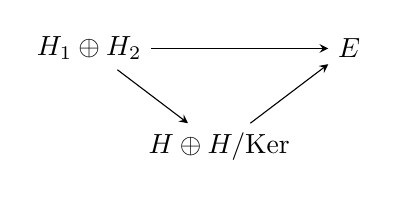
\begin{tikzpicture}[x=1cm,y=1cm,>=stealth]
\node(A)at(0,0){$H_1\oplus H_2$};
\node(B)at(3.3,0){$E$};
\node(C)at(1.65,-1.25){$H\oplus H/\mathrm{Ker}$};
\draw[->](A)--(B);\draw[->](A)--(C);\draw[->](C)--(B);
\end{tikzpicture}}\par{\footnotesize Нижние H оставлены без восстановленных индексов; штрих над Ker передан косой чертой.}}
Inf --- это как раз опр. нормы в факторпр-ве.
Но факторпр-во гильб. пр-ва само гильбертово.
Итак, это гильбертова норма.
Пусть
\begin{equation*}
H_1\subset H_2\subset E,
\end{equation*}
тогда говорим, что $H_1\leq H_2$.
[Под первым включением стрелка $i$: оператор с нормой $\leq1$.]
\begin{equation*}
\|h\|_{H_1}\geq\|h\|_{H_2}>0.
\end{equation*}
Легко пров. все св-ва:
\begin{equation*}
(\lambda\mu)H=\lambda(\mu H),\qquad
(\lambda+\mu)H=\lambda H+\mu H.
\end{equation*}
И все остальные.
\begin{equation*}
\mathcal H_1+\mathcal H_2\geq\mathcal H_1,\qquad
\lambda\mathcal H\geq\mathcal H\ \Longleftrightarrow\ \lambda\geq1.
\end{equation*}
[Справа от первого неравенства и под второй строкой густо зачёркнуты записи:
\Unclear{GELFAND-P000019}{lower-cancellations}{исходные буквы и знаки под густой штриховкой не читаются}.]
Это аксиом. \underline{выпуклого} конуса.
Сущ. необх. и дост. усл. реализации абстр. кон. структур. в
\Unclear{GELFAND-P000019}{bottom-realization}{евкл. / свкл. пр-ве [начальная буква сокращения неуверенна]}.



\Needspace{5\baselineskip}
\SourcePage{GELFAND-P000020}{unlabelled}
[Первое слово заголовка зачёркнуто: Строгий; сверху вписано: строго выпук.]
абстр. конус:
\begin{equation*}
h\geq h_1\ \Longleftrightarrow\ \exists h_2\text{ единств. (!), что }h=h_1+h_2.
\end{equation*}
Будет док., что конус гильб. подпр-в можно вложить в лин. пр-во,
в частности, вып. это усл.
Надо док., что если $H_1\leq H$, то сущ. единств. $H_2$, что $H=H_1+H_2$.
Вместо этого будет построен конус в лин. пр-ве, к-рому этот изоморфен.
\begin{equation*}
E\ \text{--- пр-во ядер},\qquad H\in\mathcal L(E^*,E).
\end{equation*}
$\mathcal L$ --- пр-во лин. опер. из антидвойств. пр-ва
(антилинейн. [зачёркнуто: \Unclear{GELFAND-P000020}{middle-cancellation}{неразборчивое короткое слово}] ф-лов) в $E$, в слабой топологии в $E$.
По опр.
\begin{equation*}
H\geq0\ \underset{\mathrm{def}}\Longleftrightarrow
\forall e^*\in E^*,\qquad (He^*\mid e^*)_{E,E^*}\geq0.
\end{equation*}
\begin{equation*}
e^*\in E^*,\quad f\in E,\qquad
(e^*\mid f)_{E^*,E}=\overline{(f\mid e^*)_{E,E^*}}.
\end{equation*}
\begin{equation*}
\mathcal L^+(E^*,E)\subset\mathcal L(E^*,E).
\end{equation*}
[Под формулой: конус положит. ядер.]
\underline{Прим.} $E$ --- гильб. пр-во,
\Unclear{GELFAND-P000020}{lower-example-symbol}{$\mathcal L^+$ [исправленный/переписанный знак неуверен]} --- полож. эрмитовы операторы.
Это строго выпуклый конус.
Конус $\mathrm{Hilb}$ ему-изоморфен.
Пусть $\mathcal H\in\mathrm{Hilb}(E)$. Надо постр. отв. ему ядро.
\begin{equation*}
e^*\in E^*;\qquad h\longmapsto(h\mid e^*)_{E,E^*}.
\end{equation*}
[Под правой частью: $e^*$ антилин.]

\clearpage\section*{Полные примечания к чтениям}
\subsection*{GELFAND-0001-U001}
\EvidenceBlock{GELFAND-P000001}{module-letter}{После A — кольцо стоит рукописная буква с развилкой сверху и нижним крюком; она повторяется у модуля и идеала.}{Наблюдение.}
\par\smallskip\noindent\textbf{Варианты: } \(\mathcal{J}\); \(\mathcal{I}\); J\par
\par\smallskip\noindent\textbf{Историческая помета: } В тексте использован каллиграфический J как графический кандидат; обозначение не определено по математическому смыслу.\par
\par\smallskip\noindent\textbf{Повторное сравнение: } В трёх отдельных вхождениях при 5×/10× видны развилка сверху и нижний крюк. Это подтверждает единое графическое обозначение,но не устанавливает однозначно условное различие I/J.\par
\subsection*{GELFAND-0001-U002}
\EvidenceBlock{GELFAND-P000001}{diagram-blowup}{В верхней половине три округлых контура с внутренними кривыми, две стрелки влево; над ними и рядом D, D', M и индексы.}{Наблюдение.}
\par\smallskip\noindent\textbf{Варианты: } Не предложены.\par
\par\smallskip\noindent\textbf{Историческая помета: } Неуверенные внутренние кривые и соединения не перерисованы. Описание и описание исходного рисунка сохраняют источник для проверки.\par
\par\smallskip\noindent\textbf{Повторное сравнение: } Полная вырезка рисунка теперь показана при его набранном описании. Видны оба наконечника стрелок влево. От нижнего контура вверх к области около D идёт отдельный изогнутый штрих; его точное соединение с верхним контуром не утверждается.\par
\subsection*{GELFAND-0001-U003}
\EvidenceBlock{GELFAND-P000001}{blowup-notation}{Верхний индекс у \(M_0\) выглядит как H; у нижней области над \(M_0\) стоит короткий штрих.}{Наблюдение.}
\par\smallskip\noindent\textbf{Варианты: } \(M_0^H\); \(M'_0\); \(M_0^N\); \(M'_0\)\par
\par\smallskip\noindent\textbf{Историческая помета: } Индексы и штрих требуют сравнения с оригиналом.\par
\par\smallskip\noindent\textbf{Повторное сравнение: } Непосредственно при чтении помещены отдельные крупные вырезки тёмного верхнего индекса и нижнего штриха. Нижний штрих различим; для тёмного верхнего знака нет достаточного основания исключить N в пользу H.\par
\subsection*{GELFAND-0001-U006}
\EvidenceBlock{GELFAND-P000001}{origin-example}{Справа от примера \(R^2\) строка начинается связной группой букв и оканчивается в 0 проект. прямой.}{Наблюдение.}
\par\smallskip\noindent\textbf{Варианты: } Вклеив. в 0 проект. прямой; Оклеив. в 0 проект. прямой\par
\par\smallskip\noindent\textbf{Историческая помета: } Фраза дана внутри пометы сомнительного чтения, без выбора по смыслу раздутия.\par
\par\smallskip\noindent\textbf{Повторное сравнение: } Широкий контекст и детали 5×/10× существенно поддерживают начальную В и сокращение «Вклеив.». Исторический вариант сохранён; формулировка не заменена стандартным определением раздутия.\par

\subsection*{GELFAND-0001-U007}
\EvidenceBlock{GELFAND-P000002}{ideal-selection}{Повторное чтение увеличенного исходного фрагмента лучше даёт мн., нач. с 1-й степени; средние штрихи сокращения нач. всё ещё не полностью различимы.}{Наблюдение.}
\par\smallskip\noindent\textbf{Кандидаты: } мн., нач. с 1-й степени; мн., к-ст. с 1-й степенью\par
\par\smallskip\noindent\textbf{Прежнее примечание: } Первый кандидат выбран по графике исходной строки; он не заменён стандартным определением Proj.\par
\par\smallskip\noindent\textbf{Новое сравнение с источником: } В полной строке и отдельных деталях 5×/10× видны конец строки и начальное «Выбр.». Раскрытие последнего как выбора либо исключения не устанавливается из конструкции. В английском тексте сокращение сохранено. В конце графика лучше поддерживает «нач.»; прежняя альтернатива сохранена.\par

\subsection*{GELFAND-0001-U008}
\EvidenceBlock{GELFAND-P000002}{open-set-notation}{При отдельном повторном просмотре первая буква после то совпадает по форме с \(O_X\) выше; вторая совпадает с буквой идеала с нижним крюком.}{Наблюдение.}
\par\smallskip\noindent\textbf{Кандидаты: } \(O_U,J_U\); \(O_U,I_U\)\par
\par\smallskip\noindent\textbf{Прежнее примечание: } Первоначальное чтение первой буквы как J исправлено по скану. Возможное различие I/J второй буквы остаётся, независимо от стандартной конструкции пучка.\par
\par\smallskip\noindent\textbf{Новое сравнение с источником: } Исправленный общий фрагмент включает нижние индексы полностью. Округлая первая буква и вторая с развилкой и нижним крюком совпадают с парой выше. Это поддерживает O и букву идеала, но не устраняет условного различия I/J. Отдельные детали просмотрены при 5×/10×.\par

\subsection*{GELFAND-0001-U009}
\EvidenceBlock{GELFAND-P000002}{fractions-sentence}{После Кольцо отношений видны числ., знамен., не прин. ни одному из идеалов, но границы сокращений и область действия последней фразы не ясны.}{Наблюдение.}
\par\smallskip\noindent\textbf{Кандидаты: } числ., знамен., не прин. ни одному из идеалов; числ.; знамен. не прин. ни одному из идеалов\par
\par\smallskip\noindent\textbf{Прежнее примечание: } Пунктуация не исправлена определением локализации.\par
\par\smallskip\noindent\textbf{Новое сравнение с источником: } Четыре перекрывающихся фрагмента сохраняют конец «числ.», следующее «знамен.» и фразу об идеалах. Сокращения видны при 5×/10×, но пунктуация не устанавливает область ограничения. Недостающее уточнение не добавлено.\par

\subsection*{GELFAND-0001-U010}
\EvidenceBlock{GELFAND-P000002}{margin-grothendieck}{Правая помета у двух вертикальных стрелок: Гротендик — раздуть ...; последнее слово написано связно.}{Наблюдение.}
\par\smallskip\noindent\textbf{Кандидаты: } идеально; идеалы\par
\par\smallskip\noindent\textbf{Прежнее примечание: } Последнее слово не утверждается.\par
\par\smallskip\noindent\textbf{Новое сравнение с источником: } Общий фрагмент содержит обе стрелки вниз и всю помету. Конечные связные штрихи скорее дают «идеально», но не исключают «идеалы». Сохранены буквальный кандидат и альтернатива; фраза не превращена в определение.\par

\subsection*{GELFAND-0001-U011}
\EvidenceBlock{GELFAND-P000002}{quadratic-coefficients}{После J тензор J толстая двусторонняя отметка и квадратный многочлен; коэффициенты похожи на \(a_2\), \(2b_2\), c.}{Наблюдение.}
\par\smallskip\noindent\textbf{Кандидаты: } \(a_2x^2+2b_2xy+cy^2+\cdots\); \(a_2x^2+2b_2xy+c_2y^2+\cdots\)\par
\par\smallskip\noindent\textbf{Прежнее примечание: } Индекс последнего коэффициента и направление толстой отметки не уверены.\par
\par\smallskip\noindent\textbf{Новое сравнение с источником: } В полном контексте и деталях видны \(a_2\) и \(2b_2\). У c-образной буквы есть малый верхний штрих, который не даёт уверенного нижнего индекса 2. Толстая связь оставлена графическим кандидатом без утверждения изоморфизма.\par

\subsection*{GELFAND-0001-U012}
\EvidenceBlock{GELFAND-P000002}{last-sign}{У нижней границы \(a_0+(a_1x-b_1y)z+\cdots\); горизонтальный знак перед \(b_1y\) выглядит как минус.}{Наблюдение.}
\par\smallskip\noindent\textbf{Кандидаты: } \(a_0+(a_1x-b_1y)z+\cdots\); \(a_0+(a_1x+b_1y)z+\cdots\)\par
\par\smallskip\noindent\textbf{Прежнее примечание: } В теле сохранён видимый минус; следующий скан имеет плюс. Стрелка слева густо написана.\par
\par\smallskip\noindent\textbf{Новое сравнение с источником: } В увеличении знак перед \(b_1y\) горизонтален; пересекающего вертикального штриха не видно. На следующей странице стоит плюс. Обе записи сохранены; возможная математическая смена знака не исправляет текст. Направление толстой стрелки остаётся сомнительным.\par

\subsection*{GELFAND-0001-U013}
\EvidenceBlock{GELFAND-P000003}{directions}{В скобках после плоскости написано сокращение замк. всеми возм. напр. — знак, похожий на сигму, процесс.}{Наблюдение.}
\par\smallskip\noindent\textbf{Кандидаты: } замк. всеми возм. напр. — σ-процесс; зам. всеми возм. напр. — σ-процесс\par
\par\smallskip\noindent\textbf{Прежнее примечание: } Сокращения не раскрыты и не заменены термином по смыслу.\par
\par\smallskip\noindent\textbf{Новое сравнение с источником: } Начальное сокращение и сигма-подобный знак просмотрены при 5×/10×. Последний короткий штрих сокращения не вполне надёжен. В переводе соседние ясные сокращения раскрыты, а «замк.» оставлено явно нераскрытым.\par

\subsection*{GELFAND-0001-U014}
\EvidenceBlock{GELFAND-P000003}{cross-cancellation}{Между В пр-ве и крестом густо зачёркнута короткая группа букв.}{Наблюдение.}
\par\smallskip\noindent\textbf{Кандидаты: } Кандидаты не предложены.\par
\par\smallskip\noindent\textbf{Прежнее примечание: } Само зачёркивание отмечено; текст под ним нельзя прочитать уверенно.\par
\par\smallskip\noindent\textbf{Новое сравнение с источником: } Плотное горизонтальное зачёркивание не читается и при 10×. Отдельный исходный крест показан рядом с имеющимся двухштриховым наборным воспроизведением. Утолщённые концы не устанавливают намеренных стрелок; оставлены две пересекающиеся линии без наконечников.\par

\subsection*{GELFAND-0001-U016}
\EvidenceBlock{GELFAND-P000003}{ising-cancellation}{Под именем Добрушин перед Найти полностью зачёркнута группа букв.}{Наблюдение.}
\par\smallskip\noindent\textbf{Кандидаты: } Кандидаты не предложены.\par
\par\smallskip\noindent\textbf{Прежнее примечание: } Видимая отмена сохранена, исходное слово не реконструировано.\par
\par\smallskip\noindent\textbf{Новое сравнение с источником: } Общий контекст устанавливает место перед «Найти»; при 5×/10× видны плотные пересекающиеся штрихи. Полного слова они не дают, поэтому кандидат не выдуман.\par

\subsection*{GELFAND-0001-U017}
\EvidenceBlock{GELFAND-P000003}{configuration-letter}{Перед \((x_1,\ldots,x_N)\) и далее в формулах знак с округлой нижней частью и тёмным верхним штрихом.}{Наблюдение.}
\par\smallskip\noindent\textbf{Кандидаты: } \(\theta\); \(b\); в\par
\par\smallskip\noindent\textbf{Прежнее примечание: } Во фрагменте применён θ как единый графический кандидат для этого повторяющегося знака.\par
\par\smallskip\noindent\textbf{Новое сравнение с источником: } Исправленный фрагмент включает знак слева и равенство целиком. Два вхождения просмотрены при 5×/10×. Разделённая петля и густой верхний штрих повторяются, но b либо кириллическая «в» надёжно не исключены. Чтение θ остаётся явно условным.\par

\subsection*{GELFAND-0001-U018}
\EvidenceBlock{GELFAND-P000003}{energy-cancellation}{Между Модель Изинга и \(U(\theta)\) находится отдельный полностью закрашенный знак.}{Наблюдение.}
\par\smallskip\noindent\textbf{Кандидаты: } Кандидаты не предложены.\par
\par\smallskip\noindent\textbf{Прежнее примечание: } Зачёркнутый знак не принят за математический оператор.\par
\par\smallskip\noindent\textbf{Новое сравнение с источником: } Знак остаётся непрозрачным при 5×/10×; тёмная масса и остатки штрихов не определяют оператор или букву. Сохранены место и зачёркивание без приписывания математической роли.\par

\subsection*{GELFAND-0001-U019}
\EvidenceBlock{GELFAND-P000003}{energy-case}{Во второй ветви u=... перед \((x_i,x_j)=1\) знак похож на ρ; ниже подпись начинается \(u(\theta)\).}{Наблюдение.}
\par\smallskip\noindent\textbf{Кандидаты: } \(\rho(x_i,x_j)=1\); \(\chi(x_i,x_j)=1\)\par
\par\smallskip\noindent\textbf{Прежнее примечание: } Виден знак после единицы, похожий на точку с запятой. Малое u в подписи не заменено на U.\par
\par\smallskip\noindent\textbf{Новое сравнение с источником: } Исправленный контекст содержит равенство целиком, а исправленная деталь 5×/10× — сам ρ-подобный знак. Прежняя узкая деталь не охватывала его и не считается свидетельством его чтения. Полная нижняя подпись начинается малой u-образной буквой. Пунктуация ветви и различие U/u сохранены; математический смысл обсуждается отдельно.\par

\subsection*{GELFAND-0001-U020}
\EvidenceBlock{GELFAND-P000003}{partition-domain}{Первая нормирующая величина выглядит \(Z(V_\ell,N)\), ниже написано \(Z(\ell,N)\); множество под второй суммой имеет форму рукописного B.}{Наблюдение.}
\par\smallskip\noindent\textbf{Кандидаты: } \(Z(V_\ell,N);\ Z(\ell,N);\ \theta\in B\); \(Z(V_\ell,N);\ Z(\ell,N);\ \theta\in\mathcal B\)\par
\par\smallskip\noindent\textbf{Прежнее примечание: } Различие аргументов сохранено. Символ множества не объявлен тождественным событию B по смыслу.\par
\par\smallskip\noindent\textbf{Новое сравнение с источником: } Отдельные детали 5×/10× подтверждают \(V_\ell\) в первом знаменателе и ell в следующей строке. У множества под второй суммой есть верхний дополнительный штрих, поддерживающий отдельный графический кандидат; обычное и каллиграфическое B всё ещё различаются неуверенно. Кандидаты события и множества конфигураций не отождествлены.\par

\subsection*{GELFAND-0001-U021}
\EvidenceBlock{GELFAND-P000003}{attraction-note}{После Молекулы притяг. скобки с закрашенными знаками, стрелками и словами соседи, вероятн.}{Наблюдение.}
\par\smallskip\noindent\textbf{Кандидаты: } соседи > их вероятн.; соседи > его вероятн.\par
\par\smallskip\noindent\textbf{Прежнее примечание: } Условная подпись передана только как кандидат, рисунок не превращён в точное утверждение.\par
\par\smallskip\noindent\textbf{Новое сравнение с источником: } Закрашенные знаки, стрелки и подпись показаны вместе. При 5×/10× местоимение ближе к «его», чем к «их», но неполная фраза не даёт точного утверждения. Унаследованный кандидат в тексте оставлен явно сомнительным; обе прежние альтернативы сохранены.\par

\subsection*{GELFAND-0001-U022}
\EvidenceBlock{GELFAND-P000003}{density-cancellation}{Перед \(V_\ell/N_\ell\) густо зачёркнута короткая отметка.}{Наблюдение.}
\par\smallskip\noindent\textbf{Кандидаты: } Кандидаты не предложены.\par
\par\smallskip\noindent\textbf{Прежнее примечание: } Первоначальный знак не восстановлен.\par
\par\smallskip\noindent\textbf{Новое сравнение с источником: } Зачёркнутая отметка не читается в увеличении. Общий фрагмент включает дробь и \(v=\mathrm{const}\), поэтому место видно. Сохранено написанное отношение \(V_\ell/N_\ell\); оно не заменено молча плотностью \(N_\ell/V_\ell\).\par


\subsection*{GELFAND-0001-U024}
\EvidenceBlock{GELFAND-P000004}{pressure-letter}{Первый аргумент \(p(\cdot,T)\) густо написан, в дроби \(\partial f/\partial v\) и перед ней T; минус перед производной не виден.}{Наблюдение.}
\par\smallskip\noindent\textbf{Кандидаты: } \(p(v,T)=T\partial f/\partial v\); \(p(\nu,T)=T\partial f/\partial v\)\par
\par\smallskip\noindent\textbf{Прежнее примечание: } Не подставлено термодинамически ожидаемое исправление знака.\par
\par\smallskip\noindent\textbf{Новое сравнение с источником: } В целом кадре и деталях 3×/5×/10× минус перед T не виден. Первый аргумент остаётся густым v-подобным знаком; \(\nu\) не исключено. Отдельный комментарий выводит возможный плюс при явно оговорённом определении f, но не выбирает букву и не исправляет источник.\par

\subsection*{GELFAND-0001-U025}
\EvidenceBlock{GELFAND-P000004}{diagram-phase-point}{Верхний правый рисунок имеет возрастающую кривую с плоской серединой, стрелку к ней и подпись точки фаз. перехода.}{Наблюдение.}
\par\smallskip\noindent\textbf{Кандидаты: } Кандидаты не предложены.\par
\par\smallskip\noindent\textbf{Прежнее примечание: } Точные оси, точки и форма переходов не указаны уверенно.\par
\par\smallskip\noindent\textbf{Новое сравнение с источником: } После исправления нижней границы фрагмента целиком видна подпись «точки фаз. перехода», во множественном числе. Оси не видны. Наборная схема передаёт плоскую середину, точку и изогнутый указатель; точное направление густого наконечника не утверждается.\par

\subsection*{GELFAND-0001-U026}
\EvidenceBlock{GELFAND-P000004}{diagram-cancelled-graph}{Слева две оси, 0 и \(\infty\) у горизонтали; несколько густо переписанных кривых и прямых, вертикальная буква.}{Наблюдение.}
\par\smallskip\noindent\textbf{Кандидаты: } вертикальная подпись \(\varphi\); вертикальная подпись f\par
\par\smallskip\noindent\textbf{Прежнее примечание: } Зачёркнутые линии сохранены описанием; точная исходная кривая не выбрана.\par
\par\smallskip\noindent\textbf{Новое сравнение с источником: } Даже при 10× отдельные соединения исходных кривых не отделяются от густых зачёркиваний. Частичная наборная схема показывает только уверенные оси, 0 и \(\infty\); спорная вертикальная буква оставлена в кандидатах. Соседний чистый график справа является другим рисунком и показан отдельно.\par

\subsection*{GELFAND-0001-U028}
\EvidenceBlock{GELFAND-P000004}{diagram-onsager}{Оси T и v; кривая с вершиной, вертикаль через вершину, \(1/2\) снизу, небольшая волнистая ветвь справа.}{Наблюдение.}
\par\smallskip\noindent\textbf{Кандидаты: } Кандидаты не предложены.\par
\par\smallskip\noindent\textbf{Прежнее примечание: } Ветви и их соединения требуют исходного рисунка; точная перерисовка не сделана.\par
\par\smallskip\noindent\textbf{Новое сравнение с источником: } Виден повторный штрих левой ветви; вертикаль проходит через вершину, под ней \(1/2\). Короткая волнистая линия справа имеет малый видимый промежуток до вершины. В наборной схеме этот промежуток сохранён, без вывода физического смысла линии.\par

\subsection*{GELFAND-0001-U029}
\EvidenceBlock{GELFAND-P000004}{kac-helfand-note}{Повторное 2-кратное увеличение строки под Kac, Helfand показывает точн. в яв. виду для нек-рых случаях; окончания слов не полностью ясны.}{Наблюдение.}
\par\smallskip\noindent\textbf{Кандидаты: } точн. в яв. виду для нек-рых случаях; точн. в яв. виде для нек-рых случаев\par
\par\smallskip\noindent\textbf{Прежнее примечание: } Слово случая... теперь прочитано, вместо ошибочного первичного сущ.; грамматика и известный результат не используются для молчаливого исправления окончания.\par
\par\smallskip\noindent\textbf{Новое сравнение с источником: } Широкий фрагмент сохраняет имена и полную строку. Детали 5×/10× лучше поддерживают «виду» и «случаях». Прежние варианты «виде» и «случаев» сохранены полностью; английский текст передаёт смысл и отдельно показывает ненормативные исходные окончания.\par

\subsection*{GELFAND-0001-U030}
\EvidenceBlock{GELFAND-P000004}{diagram-subcube}{Большой квадрат, меньшая обведённая область, в центре H, сверху h; малый контур имеет наложенные округлые и прямые штрихи.}{Наблюдение.}
\par\smallskip\noindent\textbf{Кандидаты: } Кандидаты не предложены.\par
\par\smallskip\noindent\textbf{Прежнее примечание: } Источник сохранён как рисунок, без выбора точной границы по термину подкуб.\par
\par\smallskip\noindent\textbf{Новое сравнение с источником: } И прямые, и округлые штрихи внутренней границы видны при 5×/10×; h над H читается. Внешние линии имеют промежутки. Наборная схема сохраняет наложение и промежутки, не заменяя рисунок идеальным квадратом или окружностью.\par

\subsection*{GELFAND-0001-U031}
\EvidenceBlock{GELFAND-P000004}{probability-bar}{Перед \(>\varepsilon\) видна вертикальная черта, перед первой дробью возможная левая черта сливается с фигурной скобкой.}{Наблюдение.}
\par\smallskip\noindent\textbf{Кандидаты: } \(\mathsf P\{\mu_H/h^\nu-1/v\mid>\varepsilon\}\to0\); \(\mathsf P\{|\mu_H/h^\nu-1/v|>\varepsilon\}\to0\)\par
\par\smallskip\noindent\textbf{Прежнее примечание: } Парная черта не добавлена молча; видимый кандидат оставлен в теле.\par
\par\smallskip\noindent\textbf{Новое сравнение с источником: } Правый вертикальный штрих отделён от \(>\varepsilon\). У левой фигурной скобки самостоятельная черта абсолютной величины не устанавливается даже при 10×. На следующем кадре пара черт явна, но это сравнение не меняет запись данного кадра.\par

\subsection*{GELFAND-0001-U032}
\EvidenceBlock{GELFAND-P000004}{bottom-mark}{У нижнего правого края маленький изолированный знак похож на 2 или обрывок буквы.}{Наблюдение.}
\par\smallskip\noindent\textbf{Кандидаты: } 2; обрывок буквы\par
\par\smallskip\noindent\textbf{Прежнее примечание: } Не присвоен уверенный номер страницы.\par
\par\smallskip\noindent\textbf{Новое сравнение с источником: } При 5×/10× сохраняется только короткий крючок с обрывочными штрихами у края. Цифра 2 и фрагмент буквы остаются кандидатами; номер не присвоен.\par

\subsection*{GELFAND-0001-U033}
\EvidenceBlock{GELFAND-P000004}{margin-left}{В самом левом поле кадра узкая полоса соседнего текста обрезана до отдельных окончаний и штрихов; проверен отдельный неувеличенный по пикселям crop.}{Наблюдение.}
\par\smallskip\noindent\textbf{Кандидаты: } Кандидаты не предложены.\par
\par\smallskip\noindent\textbf{Прежнее примечание: } Связный текст не доступен из этого кадра; страница имеет статус unreadable из-за этой части. Основная поверхность прочитана и транскрибирована.\par
\par\smallskip\noindent\textbf{Новое сравнение с источником: } Четыре перекрывающихся исходных полосы сохраняют весь доступный левый край. Он уже обрезан в целом исходном кадре; дополнительный масштаб не возвращает отсутствующую часть букв. Читаемые самостоятельные слова не установлены.\par

\subsection*{GELFAND-0001-U034}
\EvidenceBlock{GELFAND-P000005}{exponential-rate}{В \(O(e^{\cdots\beta})\) знак между минусом и \(\beta\) густо перекрыт; перед предыдущей фразой открывающая круглая скобка без ясно видимого закрытия.}{Наблюдение.}
\par\smallskip\noindent\textbf{Кандидаты: } \(O(e^{-N\beta})\); \(O(e^{-\ell\beta})\)\par
\par\smallskip\noindent\textbf{Прежнее примечание: } Не утверждён закрытый знак и не добавлена отсутствующая скобка исходного текста.\par
\par\smallskip\noindent\textbf{Новое сравнение с источником: } Исправленный фрагмент включает верх всех наложенных штрихов показателя. Минус и \(\beta\) видны; промежуточный знак не разделяется надёжно на N либо \(\ell\) при 10×. Отдельные фрагменты показывают вставку «отсутствия» и открывающую скобку; смысл вставки сохранён явно, скобка не закрыта редакцией.\par

\subsection*{GELFAND-0001-U035}
\EvidenceBlock{GELFAND-P000005}{complement-label}{В строке о \(\theta_2\) и \(N-k\) частицах у H виден короткий верхний штрих.}{Наблюдение.}
\par\smallskip\noindent\textbf{Кандидаты: } \(\overline H\); \(H\)\par
\par\smallskip\noindent\textbf{Прежнее примечание: } В тексте использован кандидат с чертой; дополнение не определено только по смыслу.\par
\par\smallskip\noindent\textbf{Новое сравнение с источником: } Общий фрагмент показывает оба H и горизонтальный штрих между ними. Он может быть надчеркиванием нижнего H либо подчёркиванием верхнего H; детали 5×/10× не устанавливают привязку. Прежний кандидат с надчёркиванием сохранён как кандидат, не как установленное чтение.\par

\subsection*{GELFAND-0001-U036}
\EvidenceBlock{GELFAND-P000005}{boundary-exponent}{После слов о числе гран. точек степень V записана тесно: \(\nu\)-1, косая дробная черта и \(\nu\).}{Наблюдение.}
\par\smallskip\noindent\textbf{Кандидаты: } \(V^{\nu-1/\nu}\); \(V^{(\nu-1)/\nu}\)\par
\par\smallskip\noindent\textbf{Прежнее примечание: } Первый кандидат сохранён. В следующей оценке N степень записана более явно как дробь.\par
\par\smallskip\noindent\textbf{Новое сравнение с источником: } Два фрагмента показывают тесную запись при V и явную общую дробь \((\nu-1)/\nu\) при N. Их различие сохранено. В отдельном математическом комментарии степень границы выведена для явно заданной решётчатой модели; этот вывод не превращён в чтение чернил.\par

\subsection*{GELFAND-0001-U037}
\EvidenceBlock{GELFAND-P000005}{theta-factor}{В множителе \(\exp\{\cdots N^{2/3}\}\) буква похожа на \(\theta\); ниже та же буква пояснена огранич. параметр.}{Наблюдение.}
\par\smallskip\noindent\textbf{Кандидаты: } \(\theta\); \(\Theta\)\par
\par\smallskip\noindent\textbf{Прежнее примечание: } Может отличаться от обозначения конфигурации; совпадение не объявлено доказанным.\par
\par\smallskip\noindent\textbf{Новое сравнение с источником: } В обоих множителях и подписи виден овальный знак с поперечным штрихом. Регистр \(\theta/\Theta\) и отличие от обозначения конфигурации остаются неустановленными. Степень \(2/3\) хорошо видна; её не заменяют общей степенью, записанной выше.\par

\subsection*{GELFAND-0001-U073}
\EvidenceBlock{GELFAND-P000005}{physical-meaning-heading}{Первая строка пояснения после условия фазового перехода начинается сокращением, лучше читаемым как Нагл. смысл.; средние штрихи слиты.}{Наблюдение.}
\par\smallskip\noindent\textbf{Кандидаты: } Нагл. смысл.; Нач. смысл.\par
\par\smallskip\noindent\textbf{Прежнее примечание: } Сокращение не раскрыто до полного слова; кандидат выбран по исходному фрагменту при 3x увеличении.\par
\par\smallskip\noindent\textbf{Новое сравнение с источником: } В целом слове и деталях 5×/10× лучше читается «Нагл.». Альтернатива «Нач.» и прежняя неопределённость средних штрихов сохранены; полное слово не дописано.\par

\subsection*{GELFAND-0001-U039}
\EvidenceBlock{GELFAND-P000006}{subcube-power}{В аргументе f над h стоит видимая степень 3; в следующей строке также \(\ell\)\textasciicircum{}3-h\textasciicircum{}3.}{Наблюдение.}
\par\smallskip\noindent\textbf{Кандидаты: } \(h^3/k;\ (\ell^3-h^3)/(N-k)\); \(h^\nu/k;\ (\ell^\nu-h^\nu)/(N-k)\)\par
\par\smallskip\noindent\textbf{Прежнее примечание: } Оставлена видимая тройка, без унификации с обозначением размерности \(\nu\) на соседних строках.\par
\par\smallskip\noindent\textbf{Новое сравнение с источником: } Целый кадр, два контекста и детали 5×/10× подтверждают тройки при h и \(\ell\). Чтение h\textasciicircum{}3 и \(\ell\)\textasciicircum{}3-h\textasciicircum{}3 поддерживается графически; соседнее \(\nu\) не служит основанием для замены. Исторические варианты сохранены.\par

\subsection*{GELFAND-0001-U040}
\EvidenceBlock{GELFAND-P000006}{limit-notation}{Аргумент вероятности имеет \(\mu\)\_H=k и округлый знак; справа знак плотности и две ветви с нулями. Над второй ветвью закрашенный текст.}{Наблюдение.}
\par\smallskip\noindent\textbf{Кандидаты: } \(\mu_H=k\rho;\ \rho=1/v\); \(\mu_H=k\theta;\ \rho=1/v\); \(\mu_H=k\delta;\ \delta=1/v\)\par
\par\smallskip\noindent\textbf{Прежнее примечание: } Закрашенный текст не читается. Видимые два нуля не заменены различными пределами по ожидаемому смыслу.\par
\par\smallskip\noindent\textbf{Новое сравнение с источником: } У округлой буквы после k видна нижняя загнутая ножка, что поддерживает \(\rho\); \(\theta\) и \(\delta\) остаются прежними кандидатами. Оба нуля сохраняются. Закрашенная запись над второй ветвью не восстановлена даже при 10×. Малый ступенчатый рисунок показан отдельно.\par

\subsection*{GELFAND-0001-U041}
\EvidenceBlock{GELFAND-P000006}{diagram-cell-clusters}{В большой квадратной рамке слева вертикальная цепочка заштрихованных клеток, справа угловой набор клеток.}{Наблюдение.}
\par\smallskip\noindent\textbf{Кандидаты: } Кандидаты не предложены.\par
\par\smallskip\noindent\textbf{Прежнее примечание: } Точное число клеток и внутренние отметки не уверены; исходный рисунок обязателен.\par
\par\smallskip\noindent\textbf{Новое сравнение с источником: } При сравнении готовой страницы с деталями 10× внутренние линии левой цепочки нельзя уверенно отделить от густой штриховки. Прежний новый подсчёт трёх клеток был слишком уверенным и отозван до публикации. Справа видны три клетки углом. Частичная наборная схема слева передаёт только внешний контур и штриховку; число клеток остаётся неустановленным. Оригинал сохранён рядом.\par

\subsection*{GELFAND-0001-U042}
\EvidenceBlock{GELFAND-P000006}{gamma-prime}{В двух экспонентах после равенства стоит \(\Gamma\)-подобный знак с возможным штрихом справа сверху.}{Наблюдение.}
\par\smallskip\noindent\textbf{Кандидаты: } \(\Gamma^{\prime}(\theta)\); \(\Gamma(\theta)\)\par
\par\smallskip\noindent\textbf{Прежнее примечание: } В теле передан штрихованный кандидат, несмотря на видимую подпись о длине/площади.\par
\par\smallskip\noindent\textbf{Новое сравнение с источником: } В новых деталях r3 обе буквы ближе к \(\Gamma\) без отдельного штриха; возле нижней скобки есть наложение. Первоначальные мелкие детали r2 обрезали верх и не использованы для решения о штрихе. Сохранены оба варианта и прежний кандидат тела; определение длины не подменяет чтение.\par

\subsection*{GELFAND-0001-U043}
\EvidenceBlock{GELFAND-P000006}{energy-bound}{Самая нижняя формула начинается -U(\(\theta\)), затем переписанный знак перед \(\Sigma\)(2\(\nu\)-\(\delta\)), далее 2\(\nu\)N и сумма \(\delta\) с нижним индексом \(\Gamma\)'(\(\theta\)).}{Наблюдение.}
\par\smallskip\noindent\textbf{Кандидаты: } \(-U(\theta)\ge\sum(2\nu-\delta)=2\nu N-\sum_{\Gamma^{\prime}(\theta)}\delta\)\par\smallskip\(-U(\theta)\le\sum(2\nu-\delta)=2\nu N-\sum_{\Gamma^{\prime}(\theta)}\delta\)\par\smallskip\(-U(\theta)=\sum(2\nu-\delta)=2\nu N-\sum_{\Gamma^{\prime}(\theta)}\delta\)\par
\par\smallskip\noindent\textbf{Прежнее примечание: } Не исправлена нормировка энергии по стандартной модели; индекс и последний знак также требуют проверки.\par
\par\smallskip\noindent\textbf{Новое сравнение с источником: } При 10× знак перед суммой содержит пересекающиеся штрихи и не определяет однозначно \(\ge\), \(\le\) или =. Нижний индекс последней суммы густо переписан. Отдельный подсчёт связей проверяет возможный множитель два при явных соглашениях и не исправляет эту строку.\par

\subsection*{GELFAND-0001-U044}
\EvidenceBlock{GELFAND-P000007}{diagram-small-clusters}{Малая квадратная рамка справа с двумя густыми округлыми пятнами и несколькими штрихами в верхнем левом углу.}{Наблюдение.}
\par\smallskip\noindent\textbf{Кандидаты: } Кандидаты не предложены.\par
\par\smallskip\noindent\textbf{Прежнее примечание: } Мелкие штрихи и закрашенные внутренние контуры нельзя уверенно перечислить.\par
\par\smallskip\noindent\textbf{Новое сравнение с источником: } Две крупные области и их белые просветы различимы. Вверху слева видны несколько коротких штрихов над изогнутым нижним; они не определены как заданное число частиц или букв. Частичное наборное воспроизведение сохраняет расположение и неопределённость этих отметок.\par

\subsection*{GELFAND-0001-U045}
\EvidenceBlock{GELFAND-P000007}{diagram-cycles}{В большой левой рамке три отдельные округлые группы с внутренними контурами и штриховкой, одна содержит центральный островок.}{Наблюдение.}
\par\smallskip\noindent\textbf{Кандидаты: } Кандидаты не предложены.\par
\par\smallskip\noindent\textbf{Прежнее примечание: } Вложенные циклы и штриховка не заменены приблизительно придуманной фигурой.\par
\par\smallskip\noindent\textbf{Новое сравнение с источником: } Полный контекст и новые детали различают верхнюю левую подковообразную область с открытым снизу белым промежутком, правое кольцо и нижнюю левую группу с центральным островком. Наборная схема сохраняет эту вложенность и открытый промежуток. Неровности пера и точные концы штрихов не объявлены восстановленными.\par

\subsection*{GELFAND-0001-U046}
\EvidenceBlock{GELFAND-P000007}{special-arrangement-count}{После \(\exists\) первый конечный параметр похож на N; предел суммы в условии 1 похож на M.}{Наблюдение.}
\par\smallskip\noindent\textbf{Кандидаты: } \(\exists N<\infty,\ D<\infty,\ \delta>0;\ \sum^{M}\); \(\exists M<\infty,\ D<\infty,\ \delta>0;\ \sum^{M}\)\par
\par\smallskip\noindent\textbf{Прежнее примечание: } Различие букв не устранено по повторному определению на дальнейших сканах.\par
\par\smallskip\noindent\textbf{Новое сравнение с источником: } В полном контексте первая буква остаётся ближе к N, а последующий предел — к M. Мелкая деталь r2 показывает только <\(\infty\), поэтому сама по себе не решает букву. Различие не согласовано со следующим определением.\par

\subsection*{GELFAND-0001-U047}
\EvidenceBlock{GELFAND-P000007}{large-cycles-power}{Степень длины в первом условии имеет маленькую дробную черту: \(\nu\)-1 над \(\nu\).}{Наблюдение.}
\par\smallskip\noindent\textbf{Кандидаты: } \(\ell^{(\nu-1)/\nu}\); \(\ell^{\nu-1}\)\par
\par\smallskip\noindent\textbf{Прежнее примечание: } Сохранён дробный кандидат. На GELFAND-P000010 видна степень \(\nu\)-1; она не перенесена сюда.\par
\par\smallskip\noindent\textbf{Новое сравнение с источником: } Детали 5×/10× ясно показывают дробную черту и отдельное \(\nu\) в знаменателе. Поддерживается (\(\nu\)-1)/\(\nu\). Историческая альтернатива и отличие от кадра 10 остаются в примечании; математическое ожидание поверхностной степени не меняет чернил.\par

\subsection*{GELFAND-0001-U048}
\EvidenceBlock{GELFAND-P000007}{small-cycles-sum}{У второй суммы видны верхний M и нижний i=1; подпись все ост. маленькие, после степени продолжение отсутствует.}{Наблюдение.}
\par\smallskip\noindent\textbf{Кандидаты: } \(\sum_{i=1}^{M}\Gamma_i^{\nu/(\nu-1)}\); \(\sum_{i=M+1}^{\infty}\Gamma_i^{\nu/(\nu-1)}\)\par
\par\smallskip\noindent\textbf{Прежнее примечание: } В тело внесены только видимые пределы; условие с будущего скана не дописано.\par
\par\smallskip\noindent\textbf{Новое сравнение с источником: } Контекст сохраняет верхнюю букву и подпись; детали 5×/10× подтверждают нижнее i=1. После выражения до разделительной линии продолжения нет. Сумма с i=M+1 и оценка из кадра 10 не подставлены.\par

\subsection*{GELFAND-0001-U050}
\EvidenceBlock{GELFAND-P000007}{field-margin}{Справа от уравнения несколько строк и стрелка возле \(\varphi\) и C\_0\textasciicircum{}\(\infty\); верхняя часть похожа на б, ф-й на.}{Наблюдение.}
\par\smallskip\noindent\textbf{Кандидаты: } б, ф-й на C\_0\textasciicircum{}\(\infty\); об. ф-й на C\_0\textasciicircum{}\(\infty\)\par
\par\smallskip\noindent\textbf{Прежнее примечание: } Текст не раскрыт как определение распределения по смыслу.\par
\par\smallskip\noindent\textbf{Новое сравнение с источником: } В увеличении начальный знак допускает «об.», но наложение не позволяет уверенно раскрыть сокращение. C\_0\textasciicircum{}\(\infty\) и стрелка различимы. Отдельное «\(\varphi\) — мн.» также оставлено сокращением. Определение обобщённой функции по смыслу не вставлено.\par

\subsection*{GELFAND-0001-U051}
\EvidenceBlock{GELFAND-P000007}{ideal-signature}{В строке Берём идеал, порожд. (F\_: f\(\in\)C\_0\textasciicircum{}\(\infty\)) после тире знак похож на \(\Omega\); индекс у F густо написан.}{Наблюдение.}
\par\smallskip\noindent\textbf{Кандидаты: } \(F_f;\ \Omega\); \(F_j;\ \Omega\); \(F_f;\ J\)\par
\par\smallskip\noindent\textbf{Прежнее примечание: } Обозначения остаются кандидатами и не исправлены алгебраической конструкцией.\par
\par\smallskip\noindent\textbf{Новое сравнение с источником: } Исправленный контекст доведён вправо до \(\Omega\). Знак после тире похож на широкую \(\Omega\) с нижними окончаниями. Индекс у F слит с соседними штрихами, и f остаётся предпочтением, а не установленным чтением. Алгебра не выбирает буквы.\par

\subsection*{GELFAND-0001-U052}
\EvidenceBlock{GELFAND-P000007}{evaluation-target}{После гомоморфизм в видна округлая буква с вертикальным штрихом, похожая на \(\Phi\).}{Наблюдение.}
\par\smallskip\noindent\textbf{Кандидаты: } \(\Phi\); поле, обозначенное похожей буквой\par
\par\smallskip\noindent\textbf{Прежнее примечание: } Не заменено автоматически на числовое поле.\par
\par\smallskip\noindent\textbf{Новое сравнение с источником: } При 5×/10× видны две округлые части и вертикальная ножка; \(\Phi\) графически поддерживается. Поле в дипломатической строке не дописано. Отдельный комментарий об отображении вычисления явно вводит свои предположения и не исправляет обозначение источника.\par

\subsection*{GELFAND-0001-U053}
\EvidenceBlock{GELFAND-P000008}{algebra-ring-letter}{В дроби над p тёмная буква с верхней горизонталью и округлой частью; в подписи справа похожая буква — все ур-я.}{Наблюдение.}
\par\smallskip\noindent\textbf{Кандидаты: } \(\Phi\); \(P\); \(A\)\par
\par\smallskip\noindent\textbf{Прежнее примечание: } В тексте применён \(\Phi\) как кандидат, без подстановки общепринятой буквы кольца многочленов.\par
\par\smallskip\noindent\textbf{Новое сравнение с источником: } Два отдельных фрагмента показывают числитель и подпись без уменьшения всей строки. У подписи видна округлая часть с ножкой, а числитель сильно переписан. \(\Phi\) оставлено кандидатом; обозначение привычного кольца многочленов не восстановлено по теории.\par

\subsection*{GELFAND-0001-U054}
\EvidenceBlock{GELFAND-P000008}{linear-oscillation}{Интеграл f(-\(\Box\)... )dx; знак сразу после квадрата густо перекрыт и похож на \(\varphi\), далее точки.}{Наблюдение.}
\par\smallskip\noindent\textbf{Кандидаты: } \(\int f(-\Box\varphi\ldots)\,dx\); \(\int f(-\Box\ldots)\,dx\)\par
\par\smallskip\noindent\textbf{Прежнее примечание: } Пропущенный оператор или дополнительный член не сочинён.\par
\par\smallskip\noindent\textbf{Новое сравнение с источником: } В полном контексте сохраняется густой знак сразу после \(\Box\); последующие точки в 5×/10× действительно отдельные чернильные отметки. Из них не восстановлен дополнительный член уравнения. Оба прежних чтения приведены рядом с интегралом.\par

\subsection*{GELFAND-0001-U055}
\EvidenceBlock{GELFAND-P000008}{name-van-hove}{Под пределом фамилия начинается Ван, остаток густо переписан.}{Наблюдение.}
\par\smallskip\noindent\textbf{Кандидаты: } Ван Хов; Ванхов\par
\par\smallskip\noindent\textbf{Прежнее примечание: } Пробел и последние буквы требуют проверки.\par
\par\smallskip\noindent\textbf{Новое сравнение с источником: } Начало «Ван» читается в контексте; увеличенный остаток содержит наложенные петли и не устанавливает исходный пробел и окончание. Английское имя Van Hove — передача кандидата, а не новое графическое доказательство.\par

\subsection*{GELFAND-0001-U056}
\EvidenceBlock{GELFAND-P000008}{temperature-relation}{В нижнем правом углу при T и const знак из двух горизонталей с возможным диагональным штрихом.}{Наблюдение.}
\par\smallskip\noindent\textbf{Кандидаты: } \(T=\mathrm{const}\); \(T\ne\mathrm{const}\)\par
\par\smallskip\noindent\textbf{Прежнее примечание: } Кандидат равенства не объявлен достоверным по математическому контексту.\par
\par\smallskip\noindent\textbf{Новое сравнение с источником: } Новые правильно наведённые детали r3 показывают две горизонтали; через них проходит длинная ножка верхнего слова «окр.». Поэтому равенство лучше поддерживается графически, но наложение сохранено как ограничение. Детали r2 с соседними словами не использованы как свидетельство о знаке.\par

\subsection*{GELFAND-0001-U057}
\EvidenceBlock{GELFAND-P000008}{margin-left}{На крайне левом краю кадра виден обрезанный столбик штрихов и окончаний соседней рукописи; цельные слова не видны.}{Наблюдение.}
\par\smallskip\noindent\textbf{Кандидаты: } Кандидаты не предложены.\par
\par\smallskip\noindent\textbf{Прежнее примечание: } Часть не может быть транскрибирована из доступного кадра. Основная страница прочитана; статус unreadable относится к обрезанной краевой полосе.\par
\par\smallskip\noindent\textbf{Новое сравнение с источником: } Четыре перекрывающиеся полосы сохраняют доступный край кадра. Детали нижних полос 5×/10× показывают отдельные окончания и шум границы, но не цельные слова. За пределами исходного растра данных нет; никакой отсутствующий текст не сочинён.\par

\subsection*{GELFAND-0001-U059}
\EvidenceBlock{GELFAND-P000009}{q-formula}{После Q(T)= зачёркнутый знак; далее дробь с S\_\(\nu\) e, суммой от k=2\(\nu\), 3 exp\{-1/(2T)\} с верхним k и ещё k\textasciicircum{}\{\(\nu\)/(\(\nu\)-1)\}.}{Наблюдение.}
\par\smallskip\noindent\textbf{Кандидаты: } \(\dfrac{S_\nu e(1-e^{-1/(2T)})}{3(1+e^{-\nu/T})}\sum_{k=2\nu}^{\infty}3\exp\{-1/(2T)\}^k k^{\nu/(\nu-1)}\)\par\smallskip\(\dfrac{S_\nu e(1-e^{-1/(2T)})}{3(1+e^{-\nu/T})}\sum_{k=2\nu}^{\infty}(3\exp\{-1/(2T)\})^k k^{\nu/(\nu-1)}\)\par
\par\smallskip\noindent\textbf{Прежнее примечание: } Предел суммы, область действия степени k и зачёркнутый фрагмент требуют проверки. Ожидаемая сходящаяся формула не подставлена.\par
\par\smallskip\noindent\textbf{Новое сравнение с источником: } Формула разделена на два перекрывающихся фрагмента. Детали подтверждают отдельный верхний k у закрывающей скобки и знак, похожий на \(\infty\), над суммой. Зачёркнутый фрагмент остаётся нечитаемым. Различие областей действия k математически существенно и разобрано отдельно, без выбора по сходимости.\par

\subsection*{GELFAND-0001-U060}
\EvidenceBlock{GELFAND-P000009}{sphere-constant}{В знаменателе S\_3 перед \(\sqrt{\vphantom{x}}\)\(\pi\) знак похож на C, c или цифру 6.}{Наблюдение.}
\par\smallskip\noindent\textbf{Кандидаты: } \(1/(C\sqrt\pi)\); \(1/(c\sqrt\pi)\); \(1/(6\sqrt\pi)\)\par
\par\smallskip\noindent\textbf{Прежнее примечание: } Число не восстановлено по известному объёму шара.\par
\par\smallskip\noindent\textbf{Новое сравнение с источником: } В деталях 5×/10× знак открыт вправо и лучше выглядит как C/c, чем как замкнутая 6; размер не решает прописную букву. Сохраняются три исторических варианта. Вычисленное отдельно значение для шара с площадью поверхности один не выдаётся за чтение чернил.\par

\subsection*{GELFAND-0001-U062}
\EvidenceBlock{GELFAND-P000009}{probability-brace}{После модуля дроби минус 1/v имеется \} перед >\(\varepsilon\) и ещё \} после \(\varepsilon\), затем перечёркнутая стрелка к 0.}{Наблюдение.}
\par\smallskip\noindent\textbf{Кандидаты: } \(\mathsf P\{|\mu/K_\ell^\nu-1/v|\}>\varepsilon\}\not\to0\)\par\smallskip\(\mathsf P\{|\mu/K_\ell^\nu-1/v|>\varepsilon\}\not\to0\)\par
\par\smallskip\noindent\textbf{Прежнее примечание: } Сохранены обе видимые закрывающие скобки; не исправлено обычным определением вероятностного события.\par
\par\smallskip\noindent\textbf{Новое сравнение с источником: } При 5×/10× обе закрывающие скобки различимы. Ранняя скобка не удалена ради корректного вероятностного события; обычная запись приведена только как альтернативная интерпретация. Перечёркнутая стрелка также сохранена.\par

\subsection*{GELFAND-0001-U063}
\EvidenceBlock{GELFAND-P000010}{small-cycles-sign}{В условии 2 знак перед дробью густо переписан; в верхнем пределе условия 1 буква с наложенными штрихами.}{Наблюдение.}
\par\smallskip\noindent\textbf{Кандидаты: } \(\le;\ M\); \(<;\ M\); \(\le;\ N\)\par
\par\smallskip\noindent\textbf{Прежнее примечание: } Индексы и строгость неравенства требуют сравнения; первый кандидат оставлен в теле.\par
\par\smallskip\noindent\textbf{Новое сравнение с источником: } Оба условия показаны отдельными фрагментами с верхним пределом и знаменателем S\_\(\nu\). Под знаком во втором условии видна нижняя горизонталь, поддерживающая \(\le\), но наложение сохраняется. Верхняя буква не установлена однозначно; M не перенесено из соседнего текста как доказательство.\par

\subsection*{GELFAND-0001-U064}
\EvidenceBlock{GELFAND-P000010}{small-volume-cancellation}{В скобках перед внутри мелких циклов зачёркнуто слово, над ним вставлено объём; последующие строки употребляют площ. и площадь.}{Наблюдение.}
\par\smallskip\noindent\textbf{Кандидаты: } Кандидаты не предложены.\par
\par\smallskip\noindent\textbf{Прежнее примечание: } Исходное зачёркнутое слово не читается. Площадь не заменена объёмом по размерности.\par
\par\smallskip\noindent\textbf{Новое сравнение с источником: } Три перекрывающихся фрагмента сохраняют вставку «объём», зачёркнутое слово, «заштрих. площ.» и «белая площадь». Под зачёркиванием есть петли и несколько соединений, но полное слово не установлено при 10×. Термины площади и объёма не унифицированы.\par

\subsection*{GELFAND-0001-U065}
\EvidenceBlock{GELFAND-P000010}{diagram-nested-cycles}{Округлые вложенные контуры с густо заштрихованным внешним кольцом и отдельными внутренними штрихами.}{Наблюдение.}
\par\smallskip\noindent\textbf{Кандидаты: } Кандидаты не предложены.\par
\par\smallskip\noindent\textbf{Прежнее примечание: } Точное число контуров, заштрихованные и белые компоненты требуют оригинала.\par
\par\smallskip\noindent\textbf{Новое сравнение с источником: } При 5×/10× различимы четыре вложенные границы: две у внешнего кольца и две у внутреннего. Ранее составленное описание трёх контуров уточнено в отдельном журнале изменений. Воспроизведение сохраняет четыре границы и два кольца; отдельные перьевые слияния остаются на оригинале.\par

\subsection*{GELFAND-0001-U066}
\EvidenceBlock{GELFAND-P000010}{diagram-phase-mixture}{Прямоугольник разделён кривой: сверху три округлые маленькие области, снизу штриховка и белые округлые области.}{Наблюдение.}
\par\smallskip\noindent\textbf{Кандидаты: } Кандидаты не предложены.\par
\par\smallskip\noindent\textbf{Прежнее примечание: } Точное число нижних областей и форма границы не уверены.\par
\par\smallskip\noindent\textbf{Новое сравнение с источником: } Полный фрагмент показывает три верхних пятна с белыми просветами; внизу одно замкнутое белое отверстие и ещё частично очерченная область среди штрихов. Наборная схема повторяет видимые линии, не замыкает неясную нижнюю область и не утверждает точной формы каждой границы.\par

\subsection*{GELFAND-0001-U068}
\EvidenceBlock{GELFAND-P000010}{theorem-condition}{После если вып. перед условие рукописное сокращение выглядит сформ. или строгое.}{Наблюдение.}
\par\smallskip\noindent\textbf{Кандидаты: } если вып. сформ. условие; если вып. строгое условие\par
\par\smallskip\noindent\textbf{Прежнее примечание: } Не восстановлено содержание достаточного условия из математики.\par
\par\smallskip\noindent\textbf{Новое сравнение с источником: } Полный контекст и детали 5×/10× лучше поддерживают «сформ.»: различимы округлая начальная часть и две нижние ножки в середине. Кандидат «строгое» сохранён исторически. Никакая недостающая формулировка достаточного условия не дописана.\par

\subsection*{GELFAND-0001-U069}
\EvidenceBlock{GELFAND-P000010}{diagram-grid}{Справа прямоугольная решётка с жирным квадратом в центральной клетке и подписью Разбили на подкубы.}{Наблюдение.}
\par\smallskip\noindent\textbf{Кандидаты: } Кандидаты не предложены.\par
\par\smallskip\noindent\textbf{Прежнее примечание: } Количество клеток и точное выделение не уверены; описание не задаёт придуманные координаты.\par
\par\smallskip\noindent\textbf{Новое сравнение с источником: } Исправленный фрагмент включает всю подпись. Шесть вертикальных и шесть горизонтальных линий дают сетку пять на пять; жирно выделена вторая клетка слева в четвёртом ряду сверху. Прежнее «центральной» было редакционным описанием, а не рукописным словом; оно уточнено с обратимым журналом. Масштаб клеток схемы условный.\par

\subsection*{GELFAND-0001-U070}
\EvidenceBlock{GELFAND-P000010}{last-fraction}{У нижней границы формула с густым знаком перед \(\cap\)S\_\(\ell\), знаменателем V\_\(\ell\) и \(\le\)1/v(1-\(\delta\)).}{Наблюдение.}
\par\smallskip\noindent\textbf{Кандидаты: } \((G\cap S_\ell)/V_\ell\le(1/v)(1-\delta)\); \(\operatorname{vol}(G\cap S_\ell)/V_\ell\le(1/v)(1-\delta)\)\par
\par\smallskip\noindent\textbf{Прежнее примечание: } Мера пересечения и объём подкуба не подставлены автоматически; видимый знаменатель сохранён.\par
\par\smallskip\noindent\textbf{Новое сравнение с источником: } Фрагмент продлён вниз, и новая деталь r3 сохраняет целиком V\_\(\ell\). Числитель остаётся густым G-подобным знаком; обозначение меры не видно. Следствие об усреднении по подкубам разобрано отдельно и не используется для замены знаменателя или вставки меры.\par

\subsection*{GELFAND-0001-U071}
\EvidenceBlock{GELFAND-P000006}{diagram-limit-step}{Справа от второй ветви предела маленький восходящий штрих, горизонтальный участок вправо и второй подъём на правом конце.}{Наблюдение.}
\par\smallskip\noindent\textbf{Кандидаты: } Кандидаты не предложены.\par
\par\smallskip\noindent\textbf{Прежнее примечание: } Отдельные оси, стрелки и подписи не установлены. Схема передана источниковым описанием, без подстановки типовой функции или математического значения.\par
\par\smallskip\noindent\textbf{Новое сравнение с источником: } Детали 5×/10× подтверждают восходящую линию, почти горизонтальный участок и правый подъём. Отдельных осей и надписей нет. Наборный штрих передаёт только видимую форму без названия функции и значений.\par

\subsection*{GELFAND-0001-U072}
\EvidenceBlock{GELFAND-P000009}{finite-parameter}{В строке трёх чисел первая буква имеет два высоких вертикальных штриха и толстое внутреннее соединение. После повторного просмотра при 2x и 10x она ближе к N, но M не исключено.}{Наблюдение.}
\par\smallskip\noindent\textbf{Кандидаты: } \(N<\infty,\ D<\infty,\ \delta>0\); \(M<\infty,\ D<\infty,\ \delta>0\)\par
\par\smallskip\noindent\textbf{Прежнее примечание: } Буква не определяется по ожидаемому числу контуров и не согласуется автоматически с M в сумме следующего кадра.\par
\par\smallskip\noindent\textbf{Новое сравнение с источником: } Новый узкий контекст и детали 5×/10× поддерживают N-подобную форму, но соединение густое и M остаётся вариантом. Предел суммы следующего кадра не меняет эту строку. Историческое сообщение о прежних увеличениях сохранено как прежнее, а не приписано новому просмотру.\par

\subsection*{GELFAND-0002-U001}
\EvidenceBlock{GELFAND-P000011}{top-line}{Перед глаголом окружают виден короткий двухпетлевой знак, похожий на со или \(\infty\).}{Наблюдение.}
\par\smallskip\noindent\textbf{Кандидаты: } со окружают; \(\infty\) окружают\par
\par\smallskip\noindent\textbf{Прежнее примечание: } Повторно просмотрены родной кроп 1× и увеличение 2× без сглаживания. Источник chapter\_001/01\_part\_000011.png; пиксели (820, 20, 1270, 105). Контурный контекст не определяет двухпетлевой знак или опущенный объект окружения; оба графических кандидата оставлены.\par
\par\smallskip\noindent\textbf{Новое сравнение с источником: } На целом кадре и деталях 5×/10× видна левая открытая петля, соединённая с правой. Они не позволяют однозначно различить «со» и знак бесконечности. Объект при «окружают» не дописан.\par

\subsection*{GELFAND-0002-U002}
\EvidenceBlock{GELFAND-P000011}{diagram-01}{В левом прямоугольнике четыре тёмных кружка. В правом четыре круглых знака: три с хорошо видимым светлым центром, нижний правый тёмнее; между ними дополнительные дугообразные штрихи.}{Наблюдение.}
\par\smallskip\noindent\textbf{Кандидаты: } Кандидаты не предложены.\par
\par\smallskip\noindent\textbf{Прежнее примечание: } Повторно просмотрены родной кроп 1× и увеличение 2× без сглаживания. Источник chapter\_001/01\_part\_000011.png; пиксели (450, 75, 870, 175). Контурная/вероятностная интерпретация рисунков возможна, но не даёт права менять характер кружков или дорисовывать направления штрихов.\par
\par\smallskip\noindent\textbf{Новое сравнение с источником: } При 10× различимы четыре основных знака в каждой рамке. В левых знаках есть малые белые просветы; правый нижний знак имеет меньший просвет и соседние штрихи. Частичная наборная схема сохраняет расположение четырёх знаков; мелкие внутренние штрихи оставлены на оригинале.\par

\subsection*{GELFAND-0002-U003}
\EvidenceBlock{GELFAND-P000011}{upper-middle}{Сокращение перед «границу» в строке леммы похоже на «Непрс.».}{Наблюдение.}
\par\smallskip\noindent\textbf{Кандидаты: } Непрс.; Непр.\par
\par\smallskip\noindent\textbf{Прежнее примечание: } Повторно просмотрены родной кроп 1× и увеличение 2× без сглаживания. Источник chapter\_001/01\_part\_000011.png; пиксели (490, 165, 775, 270). Оценка \(3^k\) согласуется с подсчётом вариантов по звеньям, но это не раскрывает сокращение перед границу.\par
\par\smallskip\noindent\textbf{Новое сравнение с источником: } На деталях 5×/10× видны всё сокращение, последний изогнутый штрих и точка. «Непрс.» остаётся более близким прежним кандидатом, без раскрытия в полное слово. Объяснение подсчёта дано отдельно.\par

\subsection*{GELFAND-0002-U004}
\EvidenceBlock{GELFAND-P000011}{upper-right-cancellation}{После k слово зачёркнуто и рядом вписано «звеньев».}{Наблюдение.}
\par\smallskip\noindent\textbf{Кандидаты: } точк.\par
\par\smallskip\noindent\textbf{Прежнее примечание: } Повторно просмотрены родной кроп 1× и увеличение 2× без сглаживания. Источник chapter\_001/01\_part\_000011.png; пиксели (1180, 165, 1425, 295). k звеньев естественно для контура; это лишь согласует ясно вписанное слово, а зачёркнутый кандидат точк. остаётся отдельно.\par
\par\smallskip\noindent\textbf{Новое сравнение с источником: } Вписанное «звеньев» читается. Верхняя отменённая строка и при 10× перекрыта густыми штрихами; «точк.» сохранено как кандидат, а не установленное полное слово.\par

\subsection*{GELFAND-0002-U005}
\EvidenceBlock{GELFAND-P000011}{diagram-02}{Под строкой о выигрыше/проигрыше Т-образное соединение штрихов.}{Наблюдение.}
\par\smallskip\noindent\textbf{Кандидаты: } Кандидаты не предложены.\par
\par\smallskip\noindent\textbf{Прежнее примечание: } Повторно просмотрены родной кроп 1× и увеличение 2× без сглаживания. Источник chapter\_001/01\_part\_000011.png; пиксели (495, 320, 720, 425). Т-образный штрих расположен у выигрыша/проигрыша; обозначения сторон или вероятностей из соседних экспонент не придуманы.\par
\par\smallskip\noindent\textbf{Новое сравнение с источником: } При 10× видны горизонтальный штрих, нижняя ножка и короткий отдельный отрезок справа. Стрелка и отдельная подпись не установлены. Наборная схема сохраняет правый разрыв без приписывания вероятностей ветвям.\par

\subsection*{GELFAND-0002-U006}
\EvidenceBlock{GELFAND-P000011}{middle-cancellation-01}{Короткое зачёркнутое слово после «запрещ.» перекрыто толстыми чертами.}{Наблюдение.}
\par\smallskip\noindent\textbf{Кандидаты: } не\par
\par\smallskip\noindent\textbf{Прежнее примечание: } Повторно просмотрены родной кроп 1× и увеличение 2× без сглаживания. Источник chapter\_001/01\_part\_000011.png; пиксели (1270, 525, 1470, 610). Грамматика фразы запрещ. возвращ. не определяет отменённое слово; не дано только как визуальный кандидат.\par
\par\smallskip\noindent\textbf{Новое сравнение с источником: } Начало и высокая петля сохранились, но середина при 10× густо перекрыта. Прежний кандидат «не» не объявлен достоверным и не раскрыт.\par

\subsection*{GELFAND-0002-U007}
\EvidenceBlock{GELFAND-P000011}{middle-cancellation-02}{После Каково первое зачёркнутое сокращение похоже на вер.; следующая отменённая запись сильно перекрыта.}{Наблюдение.}
\par\smallskip\noindent\textbf{Кандидаты: } вер. ...\par
\par\smallskip\noindent\textbf{Прежнее примечание: } Повторно просмотрены родной кроп 1× и увеличение 2× без сглаживания. Источник chapter\_001/01\_part\_000011.png; пиксели (430, 590, 850, 680). Вопрос о мат. ожидании делает вер. допустимым отменённым сокращением, но не восстанавливает последующее отменённое слово.\par
\par\smallskip\noindent\textbf{Новое сравнение с источником: } Две перекрывающиеся детали показывают обе отменённые части. Первая допускает «вер.»; вторая и при 10× не читается под зачёркиванием. Вопрос о вероятности не подставлен вместо написанного вопроса о математическом ожидании.\par

\subsection*{GELFAND-0002-U008}
\EvidenceBlock{GELFAND-P000011}{middle-bound}{Первый знак перед \(2{,}6^n\) содержит нижний дополнительный штрих, поэтому возможны \(\ge\) и >; далее <\(2{,}8^n\) и гипотеза \(e^n\).}{Наблюдение.}
\par\smallskip\noindent\textbf{Кандидаты: } \(\geq2{,}6^n\); \(>2{,}6^n\)\par
\par\smallskip\noindent\textbf{Прежнее примечание: } Повторно просмотрены родной кроп 1× и увеличение 2× без сглаживания. Источник chapter\_001/01\_part\_000011.png; пиксели (615, 835, 1545, 960). Экспоненциальные оценки похожи на подсчёт путей, тогда как рядом вопрос о расстоянии; предмет оценки и начальный знак не исправлены по этому рассогласованию.\par
\par\smallskip\noindent\textbf{Новое сравнение с источником: } Новая деталь подтверждает нижнее утолщение первого отношения, но не отделяет однозначно черту равенства от перьевого штриха. Оба отношения сохранены. Отдельный конечный подсчёт различает число путей и смещение, не выбирая утверждение источника.\par

\subsection*{GELFAND-0002-U009}
\EvidenceBlock{GELFAND-P000011}{bottom-line}{Последнее сокращение после «K — нелин. опер.» содержит начальную Н и окончание, похожее на «мыц.».}{Наблюдение.}
\par\smallskip\noindent\textbf{Кандидаты: } Немыц.; Намыц.\par
\par\smallskip\noindent\textbf{Прежнее примечание: } Повторно просмотрены родной кроп 1× и увеличение 2× без сглаживания. Источник chapter\_001/01\_part\_000011.png; пиксели (1320, 2240, 1590, 2365). Контекст K(u) для нелинейного уравнения допускает оператор, определяемый точечно нелинейной функцией, однако не определяет сокращение имени по одним ожидаемым буквам.\par
\par\smallskip\noindent\textbf{Новое сравнение с источником: } Начальная буква и соединённые средние штрихи видны при 10×. Гласная после Н не отделяется уверенно от соединения. Оба сокращённых имени оставлены; полное название оператора не дописано.\par

\subsection*{GELFAND-0002-U010}
\EvidenceBlock{GELFAND-P000012}{upper-norm}{Справа квадраты норм; слева после закрывающей нормы отдельный показатель не виден.}{Наблюдение.}
\par\smallskip\noindent\textbf{Кандидаты: } \(\|[\varphi,\omega]\|=\|B\varphi\|^2+\|\omega\|^2\)\par
\par\smallskip\noindent\textbf{Прежнее примечание: } Повторно просмотрены родной кроп 1× и увеличение 2× без сглаживания. Источник chapter\_001/01\_part\_000012.png; пиксели (360, 315, 1135, 445). Правая часть квадратична при масштабировании пары (\(\varphi\),ω); ожидаемый квадрат слева этим объясняется, но не добавляется без видимого показателя.\par
\par\smallskip\noindent\textbf{Новое сравнение с источником: } Деталь 5×/10× включает обе закрывающие черты нормы и свободное место показателя перед равенством. Отдельная двойка там не видна. Правые квадраты сохранены; однородность обсуждается только в отдельном математическом комментарии.\par

\subsection*{GELFAND-0002-U011}
\EvidenceBlock{GELFAND-P000012}{upper-selfadjoint}{Строка «Он не самосопр., но в этой норме самосопр.».}{Наблюдение.}
\par\smallskip\noindent\textbf{Кандидаты: } самосопр.; кососопр.\par
\par\smallskip\noindent\textbf{Прежнее примечание: } Повторно просмотрены родной кроп 1× и увеличение 2× без сглаживания. Источник chapter\_001/01\_part\_000012.png; пиксели (185, 480, 1390, 565). Матрица (0,I;−B\(^2\),0) в энергетическом скалярном произведении имеет кососопряжённую структуру, согласующуюся с \(A=-A^*\) предыдущего кадра; видимые самосопр. не заменены этим выводом.\par
\par\smallskip\noindent\textbf{Новое сравнение с источником: } Отдельные детали показывают оба вхождения с близкими начальными штрихами, в пользу «самосопр.». Матричный расчёт не превращает эти штрихи в «кососопр.»; прежняя альтернатива и расхождение источника сохранены.\par

\subsection*{GELFAND-0002-U012}
\EvidenceBlock{GELFAND-P000012}{upper-right-note}{Под записью M и от t справа подчёркнуты слова, похожие на «различные B.».}{Наблюдение.}
\par\smallskip\noindent\textbf{Кандидаты: } различные B.; разные B.\par
\par\smallskip\noindent\textbf{Прежнее примечание: } Повторно просмотрены родной кроп 1× и увеличение 2× без сглаживания. Источник chapter\_001/01\_part\_000012.png; пиксели (1600, 715, 1910, 820). Помета находится рядом с множеством решений и ссылкой (**); математический смысл не различает графически разными/различными.\par
\par\smallskip\noindent\textbf{Новое сравнение с источником: } В увеличенном слове средние штрихи сливаются перед подчёркнутым B. Вырезка сохраняет всё слово и конечное B; оба прежних словесных кандидата оставлены.\par

\subsection*{GELFAND-0002-U013}
\EvidenceBlock{GELFAND-P000012}{middle-cancellation}{В скобках о банаховом многообразии между «бан.» и «пр-ву» зачёркнута запись.}{Наблюдение.}
\par\smallskip\noindent\textbf{Кандидаты: } Кандидаты не предложены.\par
\par\smallskip\noindent\textbf{Прежнее примечание: } Повторно просмотрены родной кроп 1× и увеличение 2× без сглаживания. Источник chapter\_001/01\_part\_000012.png; пиксели (295, 900, 585, 990). Банахово многообразие и C\(\infty\) переходы не позволяют угадать отменённое слово, скрытое густыми штрихами.\par
\par\smallskip\noindent\textbf{Новое сравнение с источником: } При 10× под двумя отменяющими штрихами видны отдельные просветы, но не устойчивое полное слово. Пропущенное определение не выведено из смысла.\par

\subsection*{GELFAND-0002-U014}
\EvidenceBlock{GELFAND-P000012}{middle-right-note}{Боковая помета начинается оператор., затем мн./им. реш.; заканчивается стрелкой к H.}{Наблюдение.}
\par\smallskip\noindent\textbf{Кандидаты: } мн. реш. \(\to\) H; им. реш. \(\to\) H\par
\par\smallskip\noindent\textbf{Прежнее примечание: } Повторно просмотрены родной кроп 1× и увеличение 2× без сглаживания. Источник chapter\_001/01\_part\_000012.png; пиксели (1260, 1110, 1940, 1210). S\_t имеет область M и значения в H, поэтому мн. реш. \(\to\) H согласуется с видимой схемой; кандидат им. оставлен из-за письма.\par
\par\smallskip\noindent\textbf{Новое сравнение с источником: } Увеличенные начальные штрихи допускают «мн.», но соединения не исключают второй прежний вариант. Полный контекст показывает стрелку и H; короткая деталь относится только к начальному сокращению.\par

\subsection*{GELFAND-0002-U015}
\EvidenceBlock{GELFAND-P000012}{lower-variation}{Формула v'=Av+\(K_{u(\cdot)}\); отдельное v после последнего слагаемого не видно.}{Наблюдение.}
\par\smallskip\noindent\textbf{Кандидаты: } \(v'=Av+K_{u(\cdot)}\)\par
\par\smallskip\noindent\textbf{Прежнее примечание: } Повторно просмотрены родной кроп 1× и увеличение 2× без сглаживания. Источник chapter\_001/01\_part\_000012.png; пиксели (690, 2020, 1160, 2130). Дифференцирование \(K(u+\varepsilon v)\) по \(\varepsilon\) обычно даёт производную, применённую к v; отсутствие отдельного v на исходной строке не исправлено.\par
\par\smallskip\noindent\textbf{Новое сравнение с источником: } После закрывающей скобки при 10× видно свободное поле. Отдельный множитель v не виден. Само \(K_{u(\cdot)}\) может быть сокращённой записью; условная формула линеаризации в комментарии её не исправляет.\par

\subsection*{GELFAND-0002-U016}
\EvidenceBlock{GELFAND-P000013}{top-line}{В конце второго ряда под пунктом 3 неясное сокращение, похожее на «зд.».}{Наблюдение.}
\par\smallskip\noindent\textbf{Кандидаты: } зд.\par
\par\smallskip\noindent\textbf{Прежнее примечание: } Повторно просмотрены родной кроп 1× и увеличение 2× без сглаживания. Источник chapter\_001/01\_part\_000013.png; пиксели (680, 35, 945, 125). Список касается векторных полей и операторов, но значение/раскрытие короткого зд. из него не следует.\par
\par\smallskip\noindent\textbf{Новое сравнение с источником: } Начальная нижняя петля и конечный густой штрих при 10× остаются соединёнными. Прежнее «зд.» сохранено без раскрытия в «заданы» по смыслу предложения.\par

\subsection*{GELFAND-0002-U017}
\EvidenceBlock{GELFAND-P000013}{middle-commutator}{Третья строка коммутаторов: над второй \(\varphi\) не отделяется уверенная точка; после \(\delta\) виден дополнительный штрих; расположение x/x\(\prime\) у \(\varphi\) нечёткое.}{Наблюдение.}
\par\smallskip\noindent\textbf{Кандидаты: } \([\widetilde\varphi(x),\widetilde\varphi(x')]=i\delta'(x-x')\)\par\smallskip\([\widetilde\varphi(x),\dot{\widetilde\varphi}(x')]=i\delta(x-x')\)\par
\par\smallskip\noindent\textbf{Прежнее примечание: } Повторно просмотрены родной кроп 1× и увеличение 2× без сглаживания. Источник chapter\_001/01\_part\_000013.png; пиксели (625, 975, 1360, 1090). Предыдущая строка уже задаёт нулевой равновременной коммутатор двух полей; стандартная смешанная связь потребовала бы точки, но не доказала бы наличие точки или отсутствие штриха \(\delta\) на изображении.\par
\par\smallskip\noindent\textbf{Новое сравнение с источником: } Исправленная вырезка включает всю область тильд над обоими полями. Отдельная точка над вторым полем уверенно не видна. Штрих после \(\delta\) продолжается вниз как открывающая скобка, в пользу \(\delta\) без штриха; прежние альтернативы сохранены. Возможное сочетание двух полей без точек и \(\delta\) без штриха не заменено молча стандартным смешанным соотношением.\par

\subsection*{GELFAND-0002-U018}
\EvidenceBlock{GELFAND-P000014}{upper-borel-note}{В скобках под определением борелевского поля короткая запись перед «сод. замкн. и откр.».}{Наблюдение.}
\par\smallskip\noindent\textbf{Кандидаты: } min\par
\par\smallskip\noindent\textbf{Прежнее примечание: } Повторно просмотрены родной кроп 1× и увеличение 2× без сглаживания. Источник chapter\_001/01\_part\_000014.png; пиксели (120, 610, 435, 690). Минимальность поля согласуется с порождением открытыми/замкнутыми, но сокращение min сохранено по графике и не раскрыто.\par
\par\smallskip\noindent\textbf{Новое сравнение с источником: } Детали 5×/10× показывают соединённые штрихи, похожие на min. Кандидат оставлен сокращением; соседние слова показаны в полном контексте.\par

\subsection*{GELFAND-0002-U019}
\EvidenceBlock{GELFAND-P000014}{middle-cancellation-01}{После «Но» и перед «Рад. меры удобнее» отменены короткие слова.}{Наблюдение.}
\par\smallskip\noindent\textbf{Кандидаты: } Кандидаты не предложены.\par
\par\smallskip\noindent\textbf{Прежнее примечание: } Повторно просмотрены родной кроп 1× и увеличение 2× без сглаживания. Источник chapter\_001/01\_part\_000014.png; пиксели (350, 915, 690, 990). Преимущества Радоновых мер не определяют отменённые слова; их восстановление по смыслу не произведено.\par
\par\smallskip\noindent\textbf{Новое сравнение с источником: } При 10× видны обе отменённые группы, но густые горизонтальные и диагональные штрихи мешают полному чтению. Число групп является описанием, а не восстановленной фразой.\par

\subsection*{GELFAND-0002-U020}
\EvidenceBlock{GELFAND-P000014}{middle-uniqueness}{После Для правых мер есть сокращение перед единицы ближе к разлож., но различ. не вполне исключено; далее мера =0 на сист. окр., то она вообще ноль.}{Наблюдение.}
\par\smallskip\noindent\textbf{Кандидаты: } Для правых мер есть разлож. единицы; Для правых мер есть различ. единицы\par
\par\smallskip\noindent\textbf{Прежнее примечание: } Повторно просмотрены родной кроп 1× и увеличение 2× без сглаживания. Источник chapter\_001/01\_part\_000014.png; пиксели (205, 960, 1815, 1100). Разложение единицы могло бы объяснить переход от локального нуля меры к глобальному; это поддерживает разлож. как кандидат, а не как доказанное чтение.\par
\par\smallskip\noindent\textbf{Новое сравнение с источником: } Полный контекст 3× сохраняет всю фразу. Короткая деталь 5×/10× по средним штрихам поддерживает «разлож.», но обрезает конец слова и не является отдельным свидетельством этого окончания. Определение «правых» и обе прежние альтернативы оставлены.\par

\subsection*{GELFAND-0002-U021}
\EvidenceBlock{GELFAND-P000014}{middle-cancellation-02}{Перед «Выделим» зачёркнуто короткое слово.}{Наблюдение.}
\par\smallskip\noindent\textbf{Кандидаты: } Кандидаты не предложены.\par
\par\smallskip\noindent\textbf{Прежнее примечание: } Повторно просмотрены родной кроп 1× и увеличение 2× без сглаживания. Источник chapter\_001/01\_part\_000014.png; пиксели (765, 1190, 910, 1250). Последующее Выделим на X и Y не определяет отменённое начало.\par
\par\smallskip\noindent\textbf{Новое сравнение с источником: } Густое среднее соединение и нижняя петля сохранились, но полное слово при 10× не установлено. Отменённая запись оставлена без предположительного раскрытия.\par

\subsection*{GELFAND-0002-U022}
\EvidenceBlock{GELFAND-P000014}{lower-set-names}{В определении образа меры сначала \(A\subset Y\), затем формула с B, затем строка с B и \(A\subset X\) и формулы с A.}{Наблюдение.}
\par\smallskip\noindent\textbf{Кандидаты: } Кандидаты не предложены.\par
\par\smallskip\noindent\textbf{Прежнее примечание: } Повторно просмотрены родной кроп 1× и увеличение 2× без сглаживания. Источник chapter\_001/01\_part\_000014.png; пиксели (470, 1320, 1380, 1735). Для образа меры естественны множества в Y и их прообразы в X; видимые A/B и \(A\subset X\) тем не менее сохранены без переименования.\par
\par\smallskip\noindent\textbf{Новое сравнение с источником: } Отдельные увеличенные детали показывают \(A\subset Y\) и \(A\subset X\) с различными последними буквами. Перекрывающиеся исходные вырезки сохраняют формулу с B и следующие формулы с A. Области и обозначения не согласованы с помощью рассуждения об образе меры.\par

\subsection*{GELFAND-0002-U023}
\EvidenceBlock{GELFAND-P000014}{lower-cancellation}{Под словами о неверности обратного зачёркнуто начало строки.}{Наблюдение.}
\par\smallskip\noindent\textbf{Кандидаты: } Кандидаты не предложены.\par
\par\smallskip\noindent\textbf{Прежнее примечание: } Повторно просмотрены родной кроп 1× и увеличение 2× без сглаживания. Источник chapter\_001/01\_part\_000014.png; пиксели (225, 1850, 550, 1940). Импликация измеримости рядом не определяет перечёркнутую фразу; отменённые буквы не домыслены.\par
\par\smallskip\noindent\textbf{Новое сравнение с источником: } При 10× между длинными отменяющими штрихами видны отдельные петли, но устойчивой полной фразы они не дают. Соседняя импликация набрана отдельно.\par

\subsection*{GELFAND-0002-U024}
\EvidenceBlock{GELFAND-P000015}{upper-null-note}{Скобочная помета после «Мера одна и та же» напоминает «отлич. на мн-во вн. меры 0».}{Наблюдение.}
\par\smallskip\noindent\textbf{Кандидаты: } отлич. на мн-во вн. меры 0\par
\par\smallskip\noindent\textbf{Прежнее примечание: } Повторно просмотрены родной кроп 1× и увеличение 2× без сглаживания. Источник chapter\_001/01\_part\_000015.png; пиксели (990, 245, 1880, 330). Нулевая внешняя мера может объяснять независимость определения через E, но не заменяет неуверенную исходную скобочную фразу строгой формулировкой.\par
\par\smallskip\noindent\textbf{Новое сравнение с источником: } Начало «отлич.» и окончание «вн. меры 0» видны на перекрывающихся деталях. «вн.» не раскрыто в дипломатической записи; условное обоснование независимости дано отдельно.\par

\subsection*{GELFAND-0002-U025}
\EvidenceBlock{GELFAND-P000015}{lower-regularity}{Внизу условие \(\mu\) Rad \(\Longleftrightarrow\) \(\forall\)B комп. \(\forall\)\(\varepsilon\)>0 \(\exists\)комп., \(\mu(B-k)<\varepsilon\); после комп. отдельная буква множества и включение не видны. Второй знак в разности строчный; регистр первого не вполне уверен.}{Наблюдение.}
\par\smallskip\noindent\textbf{Кандидаты: } \(\mu(B-k)<\varepsilon\); \(\mu(b-k)<\varepsilon\)\par
\par\smallskip\noindent\textbf{Прежнее примечание: } Повторно просмотрены родной кроп 1× и увеличение 2× без сглаживания. Источник chapter\_001/01\_part\_000015.png; пиксели (1370, 1975, 1940, 2100). Внутренняя компактная регулярность обычно связывает компакт с измеримым множеством; отсутствующая буква/включение и видимые B−k не дописаны.\par
\par\smallskip\noindent\textbf{Новое сравнение с источником: } Новая деталь сохраняет всю разность и строгое неравенство. Вторая буква имеет вид k; первая ближе к B, но регистр остаётся отмеченным. Имя компакта и включение из верхнего условия не перенесены.\par

\subsection*{GELFAND-0002-U026}
\EvidenceBlock{GELFAND-P000015}{bottom-cancellation}{В отменённой фразе под горизонтальной чертой угадываются начальное св-ва и позднее бор.; уверенный конец пр-в. виден справа.}{Наблюдение.}
\par\smallskip\noindent\textbf{Кандидаты: } св-ва ... бор. ... пр-в.\par
\par\smallskip\noindent\textbf{Прежнее примечание: } Повторно просмотрены родной кроп 1× и увеличение 2× без сглаживания. Источник chapter\_001/01\_part\_000015.png; пиксели (900, 2180, 1820, 2330). Оговорка о носителе произвольной Радоновой меры не определяет густо отменённую фразу о пространствах; видимые фрагменты лишь кандидатами.\par
\par\smallskip\noindent\textbf{Новое сравнение с источником: } Две увеличенные детали показывают начальную и среднюю отменённые части. Длинные пересекающие штрихи скрывают полные слова; широкий контекст сохраняет конечное «пр-в.». Полная топологическая оговорка не восстановлена.\par

\subsection*{GELFAND-0002-U044}
\EvidenceBlock{GELFAND-P000015}{upper-lebesgue-notation}{В обозначении \(dx(E)\) обе буквы стоят на основной строке; вторая буква выглядит строчной, но её регистр не вполне различим. Та же запись повторена после слов образ её.}{Наблюдение.}
\par\smallskip\noindent\textbf{Кандидаты: } \(dx(E)\); \(dX(E)\)\par
\par\smallskip\noindent\textbf{Прежнее примечание: } Повторно просмотрены родной кроп 1× и увеличение 2× без сглаживания. Источник chapter\_001/01\_part\_000015.png; пиксели (1060, 115, 1290, 225). Нотация меры на X и лебегова мера поясняют функцию знака, но не оправдывают подстрочный индекс: dx/dX оставлены на основной строке.\par
\par\smallskip\noindent\textbf{Новое сравнение с источником: } Деталь 5×/10× ясно ставит x/X рядом с d на основной строке. Штрихи буквы крупнее части соседних строчных знаков, поэтому регистр не установлен. Подстрочный индекс не вставлен.\par

\subsection*{GELFAND-0002-U045}
\EvidenceBlock{GELFAND-P000015}{upper-regularity}{В верхнем условии \(\forall\)B \(\forall\)\(\varepsilon\)>0 \(\exists\)комп. \(\subset\)B; в разности \(\mu(b-k)\leq\varepsilon\) видны строчные буквы. Между комп. и включением отдельной буквы множества не видно.}{Наблюдение.}
\par\smallskip\noindent\textbf{Кандидаты: } \(\mu(b-k)\leq\varepsilon\)\par
\par\smallskip\noindent\textbf{Прежнее примечание: } Повторно просмотрены родной кроп 1× и увеличение 2× без сглаживания. Источник chapter\_001/01\_part\_000015.png; пиксели (1120, 855, 1940, 1040). Внутренняя регулярность объясняет математическое назначение разности, но строчные b−k и отсутствующее имя компакта не согласованы с \(\forall\)B редактором.\par
\par\smallskip\noindent\textbf{Новое сравнение с источником: } Отдельные детали сохраняют промежуток после «комп.» перед \(\subset\)B, а также всю нижнюю разность с дополнительной чертой равенства. Отсутствующее имя множества, регистры букв и нестрогое отношение оставлены как написано.\par

\subsection*{GELFAND-0002-U027}
\EvidenceBlock{GELFAND-P000016}{upper-space-symbol}{Первый символ в a(X)\(\supset\)R(X) имеет замкнутую петлю и низкое положение, ближе к строчному a; возможное A/каллиграфическая форма не исключены.}{Наблюдение.}
\par\smallskip\noindent\textbf{Кандидаты: } \(a(X)\supset R(X)\); \(A(X)\supset R(X)\)\par
\par\smallskip\noindent\textbf{Прежнее примечание: } Повторно просмотрены родной кроп 1× и увеличение 2× без сглаживания. Источник chapter\_001/01\_part\_000016.png; пиксели (360, 450, 805, 565). Контекст сравнивает абстрактные и Радоновы меры; он допускает обозначения двух классов, но не определяет регистр a/A.\par
\par\smallskip\noindent\textbf{Новое сравнение с источником: } Детали 5×/10× показывают замкнутую верхнюю петлю, нижнюю дугу и правый выходной штрих, в пользу строчного a. Само обозначение класса не определено по математическому ожиданию; A и каллиграфическая форма остаются историческими альтернативами.\par

\subsection*{GELFAND-0002-U028}
\EvidenceBlock{GELFAND-P000016}{middle-universal}{После изм. \(\forall\) слово теперь по повторному просмотру читается объемл. / объем.; надстрочная черта и окончание не вполне определены.}{Наблюдение.}
\par\smallskip\noindent\textbf{Кандидаты: } объемл. пр-ву; объем. пр-ву\par
\par\smallskip\noindent\textbf{Прежнее примечание: } Повторно просмотрены родной кроп 1× и увеличение 2× без сглаживания. Источник chapter\_001/01\_part\_000016.png; пиксели (520, 1080, 1090, 1175). Измеримость во всех объемлющих пространствах математически согласуется с универсальностью; окончание сокращения не раскрыто и надстрочный знак не нормализован.\par
\par\smallskip\noindent\textbf{Новое сравнение с источником: } На деталях 5×/10× видны соединённые средние штрихи и точка перед «пр-ву». Последний буквенный изгиб допускает «объемл.», но не устраняет прежнее «объем.»; написание и возможная верхняя черта сохранены без дипломатического раскрытия.\par

\subsection*{GELFAND-0002-U030}
\EvidenceBlock{GELFAND-P000016}{lower-operator-space}{Запись L(S,S) с пометой ф-и над/рядом с закрывающей скобкой; отдельный штрих после скобки не уверенно отделим.}{Наблюдение.}
\par\smallskip\noindent\textbf{Кандидаты: } \(L(S,S)\) [помета ф-и / note functions]; \(L(S,S)'\)\par
\par\smallskip\noindent\textbf{Прежнее примечание: } Повторно просмотрены родной кроп 1× и увеличение 2× без сглаживания. Источник chapter\_001/01\_part\_000016.png; пиксели (500, 1980, 870, 2135). Пример пространства операторов согласуется с L(S,S), но такой контекст не определяет отдельную двойственность/штрих; помета ф-и показана отдельно.\par
\par\smallskip\noindent\textbf{Новое сравнение с источником: } Полный контекст и детали 5×/10× сохраняют правую скобку и надписанное «ф-и». Отдельный уверенный штрих вне этой группы не выделяется; это не основание удалить прежний вариант со штрихом или приписать ему математическую двойственность.\par

\subsection*{GELFAND-0002-U032}
\EvidenceBlock{GELFAND-P000017}{middle-group-hypothesis}{Условие для G записано сокращённо «среди вещ. комп. нет матр. 2-го пор.».}{Наблюдение.}
\par\smallskip\noindent\textbf{Кандидаты: } вещ. комп.; матр. 2-го пор.\par
\par\smallskip\noindent\textbf{Прежнее примечание: } Повторно просмотрены родной кроп 1× и увеличение 2× без сглаживания. Источник chapter\_001/01\_part\_000017.png; пиксели (140, 1165, 1950, 1310). Контекст H¹ и деформаций указывает на условие жёсткости группы, но конкретная исключённая группа не подставлена вместо матр. 2-го пор.\par
\par\smallskip\noindent\textbf{Новое сравнение с источником: } Три перекрывающихся контекста 3× и разделённые детали 10× включают «вещ.», начало следующей строки «комп. нет матр.» и «2-го пор.». Конкретная группа, её ранг или поле не подставлены по известной формулировке теоремы.\par

\subsection*{GELFAND-0002-U033}
\EvidenceBlock{GELFAND-P000017}{lower-nondiscrete}{В предпоследнем абзаце условие «Если \(\Gamma\) не дискр.» перед упоминанием теоремы Вейля.}{Наблюдение.}
\par\smallskip\noindent\textbf{Кандидаты: } не дискр.\par
\par\smallskip\noindent\textbf{Прежнее примечание: } Повторно просмотрены родной кроп 1× и увеличение 2× без сглаживания. Источник chapter\_001/01\_part\_000017.png; пиксели (180, 2040, 1735, 2175). Строка не дискр. видна; согласование с предыдущей дискретностью \(\Gamma\) и последующей формулой размерности не даёт права менять условие.\par
\par\smallskip\noindent\textbf{Новое сравнение с источником: } Контекст 3× содержит всё «Если \(\Gamma\) не дискр.»; короткая деталь 5×/10× усиливает само «дискр.», но отрезает начало «не». Поэтому отрицание подтверждается полным контекстом, а не приписывается узкой детали. Расхождение не исправлено.\par


\subsection*{GELFAND-0002-U046}
\EvidenceBlock{GELFAND-P000017}{middle-boundary-strokes}{На горизонтальной границе большой незаписанной области сохранились только нижние части отдельных буквоподобных штрихов; целое слово не читается.}{Наблюдение.}
\par\smallskip\noindent\textbf{Кандидаты: } Кандидаты не предложены.\par
\par\smallskip\noindent\textbf{Примечание к источнику: } Просмотрены полный исходный кадр и контекст 3×, затем две перекрывающиеся детали 5× и 10× без сглаживания. Верхние части знаков отсутствуют в самом источнике. Возможное происхождение полосы и чтение слов не установлены; текст не восстановлен по догадке.\par
\par\smallskip\noindent\textbf{Новое сравнение с источником: } Просмотрены полный исходный кадр и контекст 3×, затем две перекрывающиеся детали 5× и 10× без сглаживания. Верхние части знаков отсутствуют в самом источнике. Возможное происхождение полосы и чтение слов не установлены; текст не восстановлен по догадке.\par
\subsection*{GELFAND-0002-U034}
\EvidenceBlock{GELFAND-P000018}{upper-example}{L\(^2\) включено в каллиграфическое D; толстый правый верхний знак имеет ножку/основание, похож на 1, но может быть утолщённым штрихом.}{Наблюдение.}
\par\smallskip\noindent\textbf{Кандидаты: } \(L^2\subset\mathcal D^1\); \(L^2\subset\mathcal D'\)\par
\par\smallskip\noindent\textbf{Прежнее примечание: } Повторно просмотрены родной кроп 1× и увеличение 2× без сглаживания. Источник chapter\_001/01\_part\_000018.png; пиксели (500, 810, 860, 950). L\(^2\)-функция может задавать распределение интегрированием против тестовой функции, что поддерживает D\(\prime\) математически; толстый знак всё равно допускает D¹ графически.\par
\par\smallskip\noindent\textbf{Новое сравнение с источником: } При 10× верхний знак остаётся сплошным, с выступами у основания, похожим на 1; отдельный обычный тонкий штрих не виден. Насыщенность не позволяет уверенно исключить утолщённый штрих. Оба прежних варианта оставлены, условный интегральный расчёт дан отдельно.\par

\subsection*{GELFAND-0002-U035}
\EvidenceBlock{GELFAND-P000018}{bottom-norm}{Формула нормы суммы: слева нет отчётливо видимого квадрата, справа сумма двух квадратов под inf.}{Наблюдение.}
\par\smallskip\noindent\textbf{Кандидаты: } \(\|h\|_{H_1+H_2}=\inf(\|h_1\|^2+\|h_2\|^2)\)\par
\par\smallskip\noindent\textbf{Прежнее примечание: } Повторно просмотрены родной кроп 1× и увеличение 2× без сглаживания. Источник chapter\_001/01\_part\_000018.png; пиксели (270, 2100, 1900, 2410). Inf суммы квадратов при h\(\to\)ch масштабируется как |c|\(^2\), левая норма как |c|; ожидаемый квадрат не добавлен в дипломатическую запись.\par
\par\smallskip\noindent\textbf{Новое сравнение с источником: } Детали 5×/10× включают верхнюю область над закрывающими чертами левой нормы: отдельного квадрата там не видно. В нижнем индексе между H₁ и H₂ видна запятая, а не прежний наборный плюс; она передана по источнику в сопоставленном русском тексте и переводе. Прежний кандидат сохранён в исторической записи. Формула нормы не исправлена по однородности.\par

\subsection*{GELFAND-0002-U036}
\EvidenceBlock{GELFAND-P000019}{diagram-01}{Треугольная схема прямой суммы, E и фактора по Ker; у нижних букв H индексы неразличимы.}{Наблюдение.}
\par\smallskip\noindent\textbf{Кандидаты: } \(H\oplus H/\mathrm{Ker}\); \(H_1\oplus H_2/\mathrm{Ker}\)\par
\par\smallskip\noindent\textbf{Прежнее примечание: } Повторно просмотрены родной кроп 1× и увеличение 2× без сглаживания. Источник chapter\_001/01\_part\_000019.png; пиксели (260, 380, 1250, 750). Фактор прямой суммы по ядру объясняет инъекцию в E и естественно допускает индексы 1,2, но исходные нижние H\(\oplus\)H не заменены ожидаемой формулой.\par
\par\smallskip\noindent\textbf{Новое сравнение с источником: } Расширенный контекст 3× включает три стрелки, E и полную правую помету «Получ. инъект. отобр.». Деталь 5×/10× показывает H\(\oplus\)H и косую черту над Ker; отчётливые нижние индексы у этих двух H не выделяются. Их нельзя восстанавливать из верхнего H₁\(\oplus\)H₂.\par

\subsection*{GELFAND-0002-U037}
\EvidenceBlock{GELFAND-P000019}{lower-cancellations}{Длинная густая отменённая запись справа от H1+H2\(\ge\)H1 и короткая отменённая запись под λH\(\ge\)H.}{Наблюдение.}
\par\smallskip\noindent\textbf{Кандидаты: } Кандидаты не предложены.\par
\par\smallskip\noindent\textbf{Прежнее примечание: } Повторно просмотрены родной кроп 1× и увеличение 2× без сглаживания. Источник chapter\_001/01\_part\_000019.png; пиксели (810, 1830, 1790, 2170). Аксиомы упорядоченного конуса не позволяют прочитать почти полностью закрашенные записи; обе позиции отмены учтены.\par
\par\smallskip\noindent\textbf{Новое сравнение с источником: } Обе отменённые позиции показаны в перекрывающихся контекстах 3× и отдельных деталях 5×/10×. В длинной записи сохраняются узкие просветы, в короткой — нижняя дуга, но устойчивые буквы и формулы под ними не установлены. Полные отменённые записи не придуманы из аксиом конуса.\par

\subsection*{GELFAND-0002-U038}
\EvidenceBlock{GELFAND-P000019}{bottom-realization}{Последнее сокращение перед пр-ве после реализации структуры в похоже на евкл.; свкл. не полностью исключено.}{Наблюдение.}
\par\smallskip\noindent\textbf{Кандидаты: } евкл. пр-ве; свкл. пр-ве\par
\par\smallskip\noindent\textbf{Прежнее примечание: } Повторно просмотрены родной кроп 1× и увеличение 2× без сглаживания. Источник chapter\_001/01\_part\_000019.png; пиксели (370, 2290, 940, 2390). Слово евкл. согласуется с обозначением типа пространства, но теорема о реализации не используется для исключения иных графических кандидатов.\par
\par\smallskip\noindent\textbf{Новое сравнение с источником: } Детали 5×/10× показывают начальную открытую петлю и соединение со следующей буквой, в пользу «евкл.». Полного слова в рукописи нет; исторический вариант «свкл.» оставлен без подстановки современного утверждения о реализации.\par

\subsection*{GELFAND-0002-U041}
\EvidenceBlock{GELFAND-P000020}{middle-cancellation}{В скобочном определении антидвойственного пространства зачёркнуто короткое слово перед «ф-лов».}{Наблюдение.}
\par\smallskip\noindent\textbf{Кандидаты: } Кандидаты не предложены.\par
\par\smallskip\noindent\textbf{Прежнее примечание: } Повторно просмотрены родной кроп 1× и увеличение 2× без сглаживания. Источник chapter\_001/01\_part\_000020.png; пиксели (1030, 965, 1290, 1045). Определение антидвойственности не даёт отменённого слова перед ф-лов; место отмены сохранено.\par
\par\smallskip\noindent\textbf{Новое сравнение с источником: } При 10× короткая отменённая группа остаётся плотной, с малым просветом слева. Начало следующего «ф-лов» показано для положения; из определения антилинейных функционалов отменённое слово не восстановлено.\par

\subsection*{GELFAND-0002-U042}
\EvidenceBlock{GELFAND-P000020}{lower-example-symbol}{В примере после E — гильб. пр-во знак переписан поверх прежнего; видны вертикаль, дуга и плюс.}{Наблюдение.}
\par\smallskip\noindent\textbf{Кандидаты: } \(L^+\); \(H^+\)\par
\par\smallskip\noindent\textbf{Прежнее примечание: } Повторно просмотрены родной кроп 1× и увеличение 2× без сглаживания. Источник chapter\_001/01\_part\_000020.png; пиксели (850, 1640, 1170, 1860). Положительные эрмитовы операторы согласуются с L⁺, но переписанный знак не выдаётся за уверенно прочитанный по смыслу.\par
\par\smallskip\noindent\textbf{Новое сравнение с источником: } Детали 5×/10× сохраняют перекрывающиеся вертикаль, нижнюю петлю и правый выход, рядом с ясно отделённым плюсом. Переписанная основная буква не стала однозначной; L⁺ и H⁺ оставлены, выбранное L⁺ остаётся помеченным.\par
\clearpage\section*{Математический комментарий редакции}
Следующие сравнения не исправляют дипломатический текст.

Для поля \(k\) рассмотрим \(xv=yu\) в \(\mathbb A^2_k\times\mathbb P^1_k\), с координатами \([u:v]\). В карте \(u=1\) получаем \(y=xv\), а слой над началом — аффинную \(v\)-прямую. В карте \(v=1\) имеем \(x=yu\) и аффинную \(u\)-прямую. На пересечении \(uv=1\), так что слои склеиваются в \(\mathbb P^1_k\). Вне начала \([u:v]=[x:y]\) единственно. Эта модель не устанавливает раскрытие «Выбр.», букву идеала или общее соотношение симметрической алгебры и алгебры Риса.

Для различных занятых узлов симметричная сумма по \(i\ne j\) считает каждую неупорядоченную соседнюю пару дважды. Поэтому написанное \(U\) равно минус числу таких пар; в подписи положительное число обозначено малым \(u(\theta)\). Регистр сохранён. При явно выбранных неупорядоченных конфигурациях на цепочке из четырёх узлов и двух частиц имеем \(Z=3e^{1/T}+3\); на квадрате \(2\times2\) с двумя частицами — \(Z=4e^{1/T}+2\). В обоих случаях веса, делённые на \(Z\), суммируются в единицу. Упорядочение конфигураций умножает \(Z\) на \(N!\). Написанное \(v=V_\ell/N_\ell\) — объём на частицу. Эти конечные проверки не доказывают заявленного термодинамического предела.

\subsection*{Знак давления и граничный член (исходные кадры 4–5)}
Явно предположим \(v=V/N\), \(f=N^{-1}\log Z\), \(F=-T\log Z=-TNf(V/N,T)\). При постоянных \(N,T\) цепное правило даёт
\[p=-\frac{\partial F}{\partial V}=T\frac{\partial f}{\partial v}.\]
Таким образом, при этом соглашении плюс возможен. Это не устанавливает исходное определение \(f\), букву первого аргумента или утверждения о монотонности и выпуклости.

В отдельной явно заданной решётчатой модели внутренний подкуб содержит \(h^\nu\) узлов, взаимодействие ближайших соседей имеет энергию минус единица. На каждой из \(2\nu\) граней имеется \(h^{\nu-1}\) выходящих связей. Член \(\gamma\) равен минус числу занятых связей через границу, поэтому
\[|\gamma|\le 2\nu h^{\nu-1}.\]
При фиксированных \(v=V/N\), \(V=L^\nu\), \(h/L\) это \(O(N^{(\nu-1)/\nu})\), а в размерности три — \(O(N^{2/3})\). Это возможная связь двух степеней, а не исправление тесной записи при \(V\).

При фиксированном \(k\) множество конфигураций распадается на внутренние и внешние выборы. При постоянном положительном \(T\) равномерная оценка \(|\gamma|\le CN^a\) ограничивает отношение связанной и несвязанной статистических сумм между \(e^{-CN^a/T}\) и \(e^{CN^a/T}\). Логарифм отношения даёт запись \(e^{\eta N^a}\) с ограниченным \(\eta\). Здесь коэффициент отделён от обозначения конфигурации. Исходное \(\theta/\Theta\) остаётся неустановленным.

Конечный подсчёт даёт 2, 2, 4, 8, 6 и 24 граничные связи при \((\nu,h)=(1,1),(1,3),(2,1),(2,2),(3,1),(3,2)\). При \(T=1\) перечислены также все 126 конфигураций четырёх частиц в квадрате \(3\times3\): 70 при \(k=0\) и 56 при \(k=1\) в центральном узле. Отношения сумм лежат в доказанном интервале \([1,e^4]\). Эти проверки не доказывают термодинамического предела, утверждений о фазовых переходах или чтения чернил.

\subsection*{Соглашения, подсчёт границы и неясные чернила (исходные кадры 6–10)}
Следующие вычисления используют явно указанные предположения и не заменяют неясные знаки рукописи.

В кадре 6 написано \(Z\approx e^{-Nf}\), а кадры 3 и 8 используют положительный предел \(N^{-1}\log Z\to f\). Если значение \(f\) не меняется, это разные соглашения о знаке. В дипломатическом тексте сохранены обе записи. Утверждения о выпуклости нельзя переносить между ними без проверки определений.

Для конечного занятого множества в \(\mathbb Z^\nu\) обозначим через \(E\) число неупорядоченных пар занятых ближайших соседей, через \(P\) — число граней между занятым и незанятым узлом, включая грани за пределами конечного ящика. У каждого занятого узла \(2\nu\) возможных соседей, а каждая занятая пара считается дважды, поэтому
\[2E+P=2\nu N.\]
При фиксированном \(N\) и положительном \(T\)
\[e^{E/T}=e^{\nu N/T}e^{-P/(2T)}.\]
Общий множитель сокращается при нормировке. Поэтому соглашения \(U=E\) в \(e^{U/T}\) и \(U=-E\) в \(e^{-U/T}\) дают одинаковый граничный вес. Это возможная связь кадров 6–8, а не решение о штрихе при \(\Gamma\). Если \(\delta_x\) — число отсутствующих соседей занятого узла \(x\), то \(\sum_x(2\nu-\delta_x)=2E\), а не \(E\). Переписанная энергетическая строка сохранена: её местные обозначения и знак не установлены. Перечислены все 512 подмножеств квадрата \(3\times3\) и все 256 подмножеств куба \(2\times2\times2\), включая внешние грани; тождество и нормированные веса при \(T=1\) совпадают.

Для евклидова круга с периметром один из \(2\pi r=1\) получается площадь \(1/(4\pi)\). Для трёхмерного шара с площадью поверхности один из \(4\pi r^2=1\) получается объём \(1/(6\sqrt\pi)\). Это вычисление констант шара, а не доказательство изопериметрической теоремы и не чтение густого \(C/c/6\) в кадре 9.

Положим \(q=e^{-1/(2T)}\), \(a=\nu/(\nu-1)\), где \(T>0\), \(\nu>1\). Два варианта суммы в \(Q(T)\) содержат соответственно
\[\sum_{k\ge2\nu}3q^k k^a,\qquad
 \sum_{k\ge2\nu}(3q)^k k^a.\]
Отношения соседних членов стремятся к \(q\) и \(3q\). Первый ряд сходится при любом положительном \(T\). Второй сходится тогда и только тогда, когда \(3q<1\), то есть \(T<1/(2\log3)\); при равенстве члены растут как \(k^a\), а выше не стремятся к нулю. Поэтому область действия рукописной степени существенна. Сходимость не выбирает дипломатическое чтение; критерий фазового перехода здесь не доказан.

Разобьём область объёма \(V=Km\) на \(K\) клеток одинакового объёма \(m\). Пусть \(g_j\) — объём части \(G\) в клетке \(j\), \(g=\sum_jg_j\). Тогда
\[\frac1K\sum_{j=1}^K\frac{g_j}{m}=\frac gV,\qquad
 \text{для некоторого }j:\quad\frac{g_j}{m}\le\frac gV.\]
Из \(g/V\le(1-\delta)/v\) следует оценка местной доли со знаменателем \(m\). Знаменатель \(V\), видимый внизу кадра 10, даёт другое, более слабое утверждение. Исходный знаменатель и отсутствующее обозначение меры не исправлены. Тождество усреднения проверено также во всех 625 примерах четырёх клеток объёма четыре с целыми занятыми объёмами от нуля до четырёх.

Наконец, отдельно предположим, что \(A\) — коммутативная алгебра функций над полем \(k\), содержащая постоянные функции. Вычисление в точке — гомоморфизм \(\operatorname{ev}_x:A\to k\): оно сохраняет сложение, умножение и единицу. Постоянные функции обеспечивают сюръективность, поэтому \(A/\ker\operatorname{ev}_x\cong k\), а ядро максимально. Если идеал обращается в ноль в точке, отображение проходит через фактор по нему. Это условное пояснение конструкции, а не основание заменить видимое \(\Phi\) в кадре 7 или утверждать, что всякий максимальный идеал соответствует обычному решению.


\subsection*{Блуждания, линеаризация и образы мер (исходные кадры 11--15)}
Эти условные расчёты не исправляют дипломатический текст.

На квадратной решётке после фиксированного первого ориентированного ребра путь без немедленного обратного шага имеет не более трёх возможностей для следующего ребра. Поэтому число таких слов длины $k$ не больше $3^{k-1}$ при фиксированном первом ребре и равно $4\cdot3^{k-1}$ при свободном начальном направлении. Замкнутые границы составляют подмножество этих слов с учётом способа закрепления. Это объясняет возможное появление $3^k$, но не раскрывает сокращённую лемму и не определяет её точные объекты.

Для отдельного блуждания с равномерным выбором трёх направлений, кроме немедленного обратного, обозначим единичные приращения через $D_j$, а $S_n=\sum_{j=1}^nD_j$. Условное ожидание даёт $\mathbb E(D_{j+1}\mid D_j)=D_j/3$, откуда $\mathbb E(D_i\cdot D_j)=3^{-|i-j|}$. Следовательно,
\[
\mathbb E|S_n|^2=n+2\sum_{h=1}^{n-1}(n-h)3^{-h}
=2n-\frac32+\frac32\,3^{-n},\qquad
\mathbb E|S_n|\leq\sqrt{2n}.
\]
Точное перечисление до восьми шагов подтверждает тождество. Числа самонепересекающихся путей длины от одного до восьми равны $4,12,36,100,284,780,2172,5916$, а числа путей без немедленного обратного шага равны $4\cdot3^{n-1}$. Запрет всякого посещённого узла отличается от запрета немедленного возврата. Конечные подсчёты не доказывают асимптотических оценок $2.6^n$ и $2.8^n$, не определяют смысл «возвращ.» в источнике и не выбирают оцениваемую величину.

Для конечной положительной диагональной матрицы $B$ положим $H=\operatorname{diag}(B^2,I)$ и $A=\left(\begin{smallmatrix}0&I\\-B^2&0\end{smallmatrix}\right)$. Прямое умножение даёт $A^*H+HA=0$: матрица кососопряжена в этом энергетическом скалярном произведении. Квадратичная величина $Q(\varphi,\omega)=\|B\varphi\|^2+\|\omega\|^2$ удовлетворяет $Q(cz)=|c|^2Q(z)$, а не однородности нормы степени один. Эти наблюдения не добавляют квадрат слева и не заменяют написанное «самосопр.». Для неограниченного оператора потребовался бы также анализ областей определения; конечный расчёт его не даёт.

Если дифференцируемое семейство решений удовлетворяет $u'=Au+K(u)$, дифференцирование по параметру семейства даёт $v'=Av+DK(u)[v]$. Например, для $K(u)=u^3$ имеем $DK(u)[v]=3u^2v$, поскольку
\[
\frac{(u+\varepsilon v)^3-u^3}{\varepsilon}
=3u^2v+3\varepsilon uv^2+\varepsilon^2v^3.
\]
Сокращённое $K_{u(\cdot)}$ в источнике сохранено без дописывания множителя. Аналогично, нулевой коммутатор двух полей без точек не может одновременно равняться ненулевой дельта-функции или её производной при обычной интерпретации. Эта условная проверка согласованности не устанавливает точку, штрих и аргументы рукописной строки.

Для измеримого отображения $f$ и $\nu=f_*\mu$ множество из пополнения $\nu$ лежит между измеримыми $E\subset A\subset F$, где $\nu(F\setminus E)=0$. Прообразы этих включений показывают, что $f^{-1}(A)$ принадлежит пополнению $\mu$ и имеет ту же пополненную меру. Так доказано прямое следствие при явных предположениях о пополнении, без согласования A/B и X/Y источника.

Пример источника условно объясняется так. Пусть $X\subset Y=[0,1]$ неизмеримо по Лебегу и имеет внешнюю лебегову меру один. Тогда всякое борелевское подмножество $Y\setminus X$ имеет меру ноль. Поэтому $\mu(X\cap E)=\lambda(E)$ корректно задано на следах борелевских множеств: два представителя отличаются борелевским нуль-множеством. Для непересекающихся следов пересечения представителей нулевые; последовательное удаление пересечений доказывает счётную аддитивность. При включении $i:X\to Y$ образ $i_*\mu$ совпадает с $\lambda$ на борелевских множествах. Именно $A=Y\setminus X$ неизмеримо по Лебегу, тогда как $i^{-1}(A)=\varnothing$ измерим. Это даёт нарушение обратного следствия. Само «не бор.» не означает «неизмеримо», поэтому неограниченный выбор неборелевского подмножества в источнике не принят как теорема. Общие утверждения о радоновых мерах и пополнении остаются за пределами этих элементарных проверок.


\subsection*{Гильбертовы суммы, инфинитезимальные деформации и непрерывность (исходные кадры 16--20)}
Эти сопоставления вводят дополнительные предположения и не заменяют чтения рукописи.

Для $f\in L^2(\Omega)$ и гладкой финитной пробной функции $\varphi$ имеем
\[
T_f(\varphi)=\int_\Omega f\varphi,\qquad
|T_f(\varphi)|\leq\|f\|_2\|\varphi\|_2
\leq\|f\|_2\,|K|^{1/2}\sup_K|\varphi|
\]
при $\operatorname{supp}\varphi\subset K$, где $K$ компактен. Функционал непрерывен на каждом пространстве пробных функций с фиксированным компактным носителем, как требуется для распределения. Это согласуется с возможным $\mathcal D'$, но не устанавливает штрих в густом рукописном знаке и не определяет задуманную топологию $E$.

Пусть $H_1,H_2$ непрерывно включены в хаусдорфово топологическое векторное пространство $E$. Отображение $J:H_1\oplus H_2\to E$, $J(u,v)=u+v$, имеет замкнутое ядро $N$. Факторнорма удовлетворяет
\[
\|h\|_{\mathrm{quot}}^2
=\inf_{u+v=h}\bigl(\|u\|_{H_1}^2+\|v\|_{H_2}^2\bigr).
\]
Каждый аффинный слой есть сдвиг замкнутого подпространства $N$; единственный элемент слоя, ортогональный $N$, минимизирует квадрат нормы прямой суммы. Отображение $(H_1\oplus H_2)/N\to E$ инъективно по определению $N$. Это условно объясняет треугольную схему, не дописывая нижних индексов. Для $H_1=H_2=\mathbb C$ с обычной нормой минимум равен $|h|^2/2$ при $u=v=h/2$. Дипломатическая формула сохраняет отсутствие видимого квадрата и исходную запятую в нижнем индексе.

При $\lambda,\mu>0$ тождество
\[
\frac{|x|^2}{\lambda}+\frac{|h-x|^2}{\mu}
=\frac{|h|^2}{\lambda+\mu}
+\frac{\lambda+\mu}{\lambda\mu}
 \left|x-\frac{\lambda h}{\lambda+\mu}\right|^2
\]
объясняет $(\lambda+\mu)H=\lambda H+\mu H$ при указанном обратном масштабировании скалярного произведения; то же выделение квадрата работает для гильбертовых норм. Порядок включения даёт $\|h\|_{H_2}\leq\|h\|_{H_1}$, а разложение $h=h+0$ даёт $H_1+H_2\geq H_1$. Строгая положительность нормы требует $h\ne0$. Аналогично, $\lambda H\geq H$ равносильно $\lambda\geq1$ для ненулевого $H$; при $H=0$ сравнение верно при любом $\lambda\geq0$. Эти уточнения не исправляют исходные неравенства.

В словах об общем модуле существенны кванторы. На $[0,1]$ придадим функции $f_n(t)=nt$ вероятность $2^{-n}$ при $n\geq1$. Все реализации непрерывны, закон сосредоточен на счётном объединении конечных компактных множеств. Однако всякое множество вероятности один содержит все атомы $f_n$. При любом фиксированном $\delta>0$ их приращения $n\delta$ неограниченны. Поэтому у такого семейства полной меры нет единого конечного детерминированного модуля, стремящегося к нулю. Это различает детерминированный общий модуль, отдельные и случайные модули, не подменяя сокращённую исходную фразу.

Для дифференцируемого семейства матричных представлений $\rho_t$ положим
$u(g)=\dot\rho_0(g)\rho_0(g)^{-1}$. Дифференцирование
$\rho_t(gh)=\rho_t(g)\rho_t(h)$ даёт
\[
u(gh)=u(g)+\operatorname{Ad}_{\rho_0(g)}u(h).
\]
При сопряжении $\rho_t(g)=a_t\rho_0(g)a_t^{-1}$, где $a_0=I$ и $v=\dot a_0$, получаем $u(g)=v-\operatorname{Ad}_{\rho_0(g)}v$. Это элементарный расчёт коцикла и кограницы, поясняющий обсуждение $H^1$. Он не доказывает глобальную жёсткость, не восстанавливает условие о группе и не меняет написанное «не дискр.».

Наконец, в конечномерном конусе положительных операторов равенство $A=B+C$ однозначно задаёт $C=A-B$, если разность положительна. Это сокращение в упорядоченном линейном пространстве. Оно отличается от обычного геометрического требования отсутствия нетривиальных граничных отрезков: в размерности три различные положительные матрицы следа один $\operatorname{diag}(1,0,0)$ и $\operatorname{diag}(0,1,0)$ соединены целым отрезком вырожденных матриц. Исходные слова «строго выпуклый» сохранены. Общая теорема о реализации гильбертовых ядер, универсальная измеримость и утверждения о ядерных пространствах этими элементарными сопоставлениями не доказаны.

\end{document}
